% =====================================================================
% main.tex
% Responsabilidad única: ensamblar el informe a partir de los módulos
% (preámbulo, portada, secciones y apéndice). No contiene texto propio.
%
% Para compilar:  make pdf   (o latexmk -pdf main.tex)
% Las cifras y tablas vienen de generado/ (make notebooks en la raíz).
% =====================================================================
\documentclass[11pt]{article}

% =====================================================================
% preambulo.tex
% Responsabilidad única: cargar paquetes y definir la configuración y los
% estilos reutilizables del informe (idioma, convención numérica, tablas,
% figuras, enlaces, pie institucional y macros de resultados). No contiene
% contenido propio del proyecto.
% =====================================================================

\usepackage[utf8]{inputenc}
\usepackage[T1]{fontenc}
\usepackage{lmodern}
% es-tabla: los cuadros se titulan "Tabla"; es-nodecimaldot: punto decimal
% en matemáticas (convención de todo el documento: punto decimal, sin
% separador de miles, igual que en las macros generadas).
\usepackage[spanish,es-noshorthands,es-tabla,es-nodecimaldot]{babel}
\renewcommand{\tablename}{Tabla}
\renewcommand{\listtablename}{Índice de tablas}
\usepackage[a4paper,margin=2.3cm]{geometry}
\usepackage{microtype}
\setlength{\emergencystretch}{2em}

% --- Índice: espacio para números de sección de dos cifras ---------------------
\usepackage[titles]{tocloft}
\setlength{\cftsecnumwidth}{2.1em}

% --- Matemáticas ------------------------------------------------------
\usepackage{amsmath}
\usepackage{amssymb}
\usepackage{mathtools}

% --- Tablas y figuras ---------------------------------------------------
\usepackage{graphicx}
\usepackage{adjustbox}
\graphicspath{{../figuras/}}
\usepackage{booktabs}
\usepackage{array}
\usepackage{caption}
\captionsetup{font=small, labelfont=bf, margin=0.5cm}
\usepackage{float}
\usepackage{enumitem}
\setlist{itemsep=2pt, topsep=4pt}

% --- Diagramas vectoriales -----------------------------------------------
\usepackage{tikz}
\usetikzlibrary{arrows.meta, positioning, calc}
% Misma paleta que las figuras de matplotlib del proyecto.
\definecolor{classblue}{HTML}{4C72B0}
\definecolor{classred}{HTML}{C44E52}
\definecolor{classgreen}{HTML}{55A868}
\definecolor{classorange}{HTML}{DD8452}

% --- Color y enlaces ----------------------------------------------------
\usepackage{xcolor}
\definecolor{urosariored}{RGB}{255,11,38}
\usepackage{hyperref}
\hypersetup{
    colorlinks = true,
    linkcolor  = urosariored!75!black,
    citecolor  = urosariored!75!black,
    urlcolor   = urosariored!75!black,
    pdftitle   = {Analítica predictiva sobre la base de muestras de un laboratorio de microbiología},
    pdfauthor  = {Tania Fernanda Mora Cubillos, Over Haider Castrillón Valencia y Daniel Arias Mutis},
}

% --- Espaciado de tablas y párrafos ---------------------------------------
\renewcommand{\arraystretch}{1.2}
\setlength{\parskip}{0.3em}
\setlength{\parindent}{0pt}

% --- Colocación de flotantes (menos páginas a medio llenar) -----------------
\renewcommand{\topfraction}{0.9}
\renewcommand{\bottomfraction}{0.8}
\renewcommand{\textfraction}{0.07}
\renewcommand{\floatpagefraction}{0.8}
\setcounter{topnumber}{3}
\setcounter{totalnumber}{5}
\setlength{\textfloatsep}{10pt plus 2pt minus 4pt}
\setlength{\floatsep}{8pt plus 2pt minus 2pt}

% --- Pie de página institucional -----------------------------------------
\usepackage{fancyhdr}
\pagestyle{fancy}
\fancyhf{}
\renewcommand{\headrulewidth}{0pt}
\renewcommand{\footrulewidth}{0pt}
\fancyfoot[C]{\thepage}
\fancyfoot[R]{
\includegraphics[height=0.42cm]{figuras/logo_urosario_icono.png}}

% --- Atajos de redacción ----------------------------------------------------
% Identificadores en monoespaciada que pueden cortarse después de cada "_"
% (los nombres de columna largos no caben en la línea y no se separan en sílabas).
\newcommand{\guionbajocortable}{\textunderscore\allowbreak}
\newcommand{\codigo}[1]{{\let\_\guionbajocortable\texttt{#1}}}
% Tabla generada: \tablagen{nombre}; \tablaancha la escala al ancho del texto;
% \tablacompacta la pone en letra pequeña con columnas más juntas y solo la
% reduce si aún no cabe, para que la letra no baje de unos 8 pt.
\newcommand{\tablagen}[1]{\input{generado/tabla_#1}}
\newcommand{\tablaancha}[1]{\resizebox{\textwidth}{!}{\input{generado/tabla_#1}}}
\newcommand{\tablacompacta}[1]{{\footnotesize\setlength{\tabcolsep}{3pt}%
  \adjustbox{max width=\textwidth}{\input{generado/tabla_#1}}}}

% --- Cifras generadas por los notebooks -------------------------------------
% generado/resultados.tex define una macro \NombreDeCifra por cada número
% citado (punto decimal, sin separador de miles). Si aún no existe (notebooks
% sin ejecutar), el documento compila igual con las macros indefinidas.
\IfFileExists{generado/resultados.tex}{% Generado por la construcción de los notebooks (no editar a mano).
% Cifras citadas en el informe; el índice comentado está en indice_macros.tex.

% --- 01_datos_exploracion ---
\newcommand{\DatBloquesCV}{4}
\newcommand{\DatClientes}{220}
\newcommand{\DatClientesConMuestras}{219}
\newcommand{\DatColumnasContrato}{65}
\newcommand{\DatColumnasObligatorias}{15}
\newcommand{\DatColumnasOpcionales}{50}
\newcommand{\DatControles}{26236}
\newcommand{\DatCortePrueba}{2026-01-01}
\newcommand{\DatCorteValidacion}{2025-07-01}
\newcommand{\DatCostoFN}{5}
\newcommand{\DatCostoFP}{1}
\newcommand{\DatDesde}{2023-01-02}
\newcommand{\DatDiasCalendario}{1398}
\newcommand{\DatDuplicadas}{148}
\newcommand{\DatFaltanOpcionales}{0}
\newcommand{\DatFechaFin}{2026-10-30}
\newcommand{\DatFechaInicio}{2023-01-02}
\newcommand{\DatHasta}{2026-10-30}
\newcommand{\DatHuella}{f82dd7cc9bcb}
\newcommand{\DatMomentos}{9}
\newcommand{\DatMuestrasCrudas}{38994}
\newcommand{\DatOrigen}{simulacion}
\newcommand{\DatRecuentosNoNumericos}{28716}
\newcommand{\DatRecuentosNoNumericosPct}{75.9}
\newcommand{\DatSemilla}{42}
\newcommand{\DatTablasContrato}{4}
\newcommand{\DatValoresImposiblesCrudos}{366}
\newcommand{\DatValoresImposiblesEnDuplicadas}{1}
\newcommand{\DatVisitas}{1812}
\newcommand{\ExpCVSemanal}{0.30}
\newcommand{\ExpCategoriaMasNiveles}{codigo\_producto}
\newcommand{\ExpClientesDesarrollo}{203}
\newcommand{\ExpClientesMitad}{28}
\newcommand{\ExpClientesMitadPct}{13.8}
\newcommand{\ExpColumnasConFaltantes}{25}
\newcommand{\ExpColumnasIntegradas}{69}
\newcommand{\ExpColumnasSoloEstructural}{17}
\newcommand{\ExpConformesPorNoConforme}{11}
\newcommand{\ExpDecimoClientesPct}{41.1}
\newcommand{\ExpDiferenciaEstandarMax}{0.34}
\newcommand{\ExpDuplicadosEliminados}{148}
\newcommand{\ExpEnsayoMasTardio}{mohos y levaduras}
\newcommand{\ExpEnsayoMasTardioPct}{16.6}
\newcommand{\ExpEnsayoMenosTardio}{Staphylococcus aureus}
\newcommand{\ExpEnsayoMenosTardioPct}{8.8}
\newcommand{\ExpEntregaMediana}{6}
\newcommand{\ExpEntregaPNoventa}{12}
\newcommand{\ExpEntregaTardiaPct}{12.6}
\newcommand{\ExpFilasEntrenamiento}{23151}
\newcommand{\ExpFilasPrueba}{8947}
\newcommand{\ExpFilasValidacion}{6748}
\newcommand{\ExpHorasCuartoAltoPct}{12.6}
\newcommand{\ExpHorasCuartoBajoPct}{7.0}
\newcommand{\ExpIndiceMesAlto}{1.26}
\newcommand{\ExpIndiceMesBajo}{0.83}
\newcommand{\ExpMedianaMuestrasCliente}{73}
\newcommand{\ExpMesAlto}{nov}
\newcommand{\ExpMesBajo}{ene}
\newcommand{\ExpMuestrasCrudas}{38994}
\newcommand{\ExpMuestrasDesarrollo}{29899}
\newcommand{\ExpMuestrasLimpias}{38846}
\newcommand{\ExpMuestrasSemana}{192}
\newcommand{\ExpMuestrasSemanaMax}{366}
\newcommand{\ExpMuestrasSemanaMin}{61}
\newcommand{\ExpNivelesCategoria}{1169}
\newcommand{\ExpParCorrelacionado}{dias\_prometidos y limite\_ufc}
\newcommand{\ExpPeorFaltanteColumna}{actividad\_agua}
\newcommand{\ExpPeorFaltantePct}{9.8}
\newcommand{\ExpPrimerAnio}{2023}
\newcommand{\ExpProblemaMayor}{recuento censurado (``<N'' o ``>N'')}
\newcommand{\ExpProblemaMayorFilas}{18816}
\newcommand{\ExpReglasConHallazgos}{18}
\newcommand{\ExpRhoObjetivo}{0.07}
\newcommand{\ExpRhoPar}{$-$0.28}
\newcommand{\ExpSectorMayor}{cosmético}
\newcommand{\ExpSectorMayorPct}{36.3}
\newcommand{\ExpSectorMenor}{central de mezclas}
\newcommand{\ExpSectorMenorPct}{8.6}
\newcommand{\ExpSemanas}{157}
\newcommand{\ExpTablasLimpias}{5}
\newcommand{\ExpTasaMensualMaxPct}{12.7}
\newcommand{\ExpTasaMensualMinPct}{5.5}
\newcommand{\ExpTasaNoConformePct}{8.6}
\newcommand{\ExpTasaPrimerAnioPct}{7.9}
\newcommand{\ExpTasaRechazoPct}{3.0}
\newcommand{\ExpTasaUltimoAnioPct}{8.7}
\newcommand{\ExpTemperaturaCuartoAltoPct}{12.8}
\newcommand{\ExpTemperaturaCuartoBajoPct}{6.9}
\newcommand{\ExpUltimoAnio}{2025}
\newcommand{\ExpVariableCorrObjetivo}{actividad\_agua}
\newcommand{\ExpVariableMasSepara}{horas\_transporte}

% --- 02_base_real ---
\newcommand{\RealArbolGiniAntes}{0.0690}
\newcommand{\RealArbolGiniDespues}{0.0666}
\newcommand{\RealArbolGiniReduccion}{0.0023}
\newcommand{\RealArbolPrimerCorte}{tasa\_cliente > 0.0735105}
\newcommand{\RealCalcIntercepto}{$-$3.677}
\newcommand{\RealCalcLogit}{2.047}
\newcommand{\RealCalcMayor}{tasa\_cliente}
\newcommand{\RealCalcMayorAporte}{5.442}
\newcommand{\RealCalcProba}{0.886}
\newcommand{\RealCalcTerminos}{9}
\newcommand{\RealCampanaMuestrasMediana}{14}
\newcommand{\RealCampanaUnDiaPct}{69}
\newcommand{\RealCampanas}{385}
\newcommand{\RealClientes}{82}
\newcommand{\RealClientesDispersion}{28}
\newcommand{\RealClientesPlanta}{8}
\newcommand{\RealClientesProducto}{22}
\newcommand{\RealCompuestoPlanta}{59.98}
\newcommand{\RealCompuestoProducto}{6.00}
\newcommand{\RealCongeladoHuella}{10900224adf7}
\newcommand{\RealCongeladoModelo}{Regresión logística (C = 0.01)}
\newcommand{\RealCostoFN}{5}
\newcommand{\RealCostoFP}{1}
\newcommand{\RealDesde}{2024-06-04}
\newcommand{\RealDispLotesPlanta}{1.20}
\newcommand{\RealDispLotesProducto}{0.73}
\newcommand{\RealDispLotesTodos}{0.90}
\newcommand{\RealDispMuestrasMax}{407}
\newcommand{\RealDispMuestrasPlanta}{71.16}
\newcommand{\RealDispMuestrasProducto}{4.25}
\newcommand{\RealDispMuestrasTodos}{7.23}
\newcommand{\RealFilas}{120114}
\newcommand{\RealHasta}{2025-12-19}
\newcommand{\RealHojaFilas}{51}
\newcommand{\RealHojaFraccion}{0.314}
\newcommand{\RealHojaVeces}{8.8}
\newcommand{\RealLoteDeltaGeoPlanta}{448}
\newcommand{\RealLoteDeltaGeoProducto}{5.4}
\newcommand{\RealLoteMaxPlanta}{675}
\newcommand{\RealLoteMaxProducto}{60}
\newcommand{\RealLoteMediaPlanta}{18.7}
\newcommand{\RealLoteMediaProducto}{4.1}
\newcommand{\RealLoteMedianaPlanta}{6}
\newcommand{\RealLoteMedianaProducto}{3}
\newcommand{\RealLoteMejorPlanta}{1 + binomial negativa}
\newcommand{\RealLoteMejorProducto}{1 + binomial negativa}
\newcommand{\RealLoteRPlanta}{0.39}
\newcommand{\RealLoteRProducto}{0.88}
\newcommand{\RealLotes}{2543}
\newcommand{\RealLotesPlanta}{762}
\newcommand{\RealLotesProducto}{1781}
\newcommand{\RealMinimoLotes}{20}
\newcommand{\RealMuestras}{21549}
\newcommand{\RealNivel}{0.05}
\newcommand{\RealNoConformePct}{3.7}
\newcommand{\RealOddsBaja}{previas\_lote}
\newcommand{\RealOddsBajaValor}{0.70}
\newcommand{\RealOddsSube}{tasa\_cliente}
\newcommand{\RealOddsSubeValor}{1.76}
\newcommand{\RealPlantaPct}{66.2}
\newcommand{\RealPruebaAP}{0.072}
\newcommand{\RealPruebaAPConocidos}{0.073}
\newcommand{\RealPruebaAPInf}{0.059}
\newcommand{\RealPruebaAPNuevos}{0.097}
\newcommand{\RealPruebaAPRegla}{0.064}
\newcommand{\RealPruebaAPReglaInf}{0.053}
\newcommand{\RealPruebaAPReglaSup}{0.081}
\newcommand{\RealPruebaAPSup}{0.091}
\newcommand{\RealPruebaAUC}{0.769}
\newcommand{\RealPruebaAUCInf}{0.743}
\newcommand{\RealPruebaAUCSup}{0.794}
\newcommand{\RealPruebaClientes}{72}
\newcommand{\RealPruebaClientesNuevos}{17}
\newcommand{\RealPruebaCosto}{1718}
\newcommand{\RealPruebaCostoNada}{1710}
\newcommand{\RealPruebaFN}{339}
\newcommand{\RealPruebaFP}{23}
\newcommand{\RealPruebaFUno}{0.016}
\newcommand{\RealPruebaMuestras}{16325}
\newcommand{\RealPruebaNuevasPct}{29}
\newcommand{\RealPruebaPositivos}{342}
\newcommand{\RealPruebaPrecision}{0.115}
\newcommand{\RealPruebaPrevalencia}{0.021}
\newcommand{\RealPruebaPrevalenciaPct}{2.1}
\newcommand{\RealPruebaRecall}{0.009}
\newcommand{\RealPruebaSinHistoriaPct}{2.2}
\newcommand{\RealPruebaTN}{15960}
\newcommand{\RealPruebaTP}{3}
\newcommand{\RealPruebaVeces}{3.4}
\newcommand{\RealRiesgoAPArbol}{0.073}
\newcommand{\RealRiesgoAPArbolProfundoEnt}{0.212}
\newcommand{\RealRiesgoAPArbolProfundoVal}{0.073}
\newcommand{\RealRiesgoAPBase}{0.041}
\newcommand{\RealRiesgoAPElegido}{0.109}
\newcommand{\RealRiesgoAPHistoria}{0.105}
\newcommand{\RealRiesgoAPLogistica}{0.109}
\newcommand{\RealRiesgoAPLogisticaEnt}{0.114}
\newcommand{\RealRiesgoAUCArbol}{0.683}
\newcommand{\RealRiesgoAUCElegido}{0.689}
\newcommand{\RealRiesgoAUCHistoria}{0.673}
\newcommand{\RealRiesgoAUCLogistica}{0.689}
\newcommand{\RealRiesgoArbol}{profundidad 5}
\newcommand{\RealRiesgoElegido}{Regresión logística (C = 0.01)}
\newcommand{\RealRiesgoEntrenamiento}{15628}
\newcommand{\RealRiesgoEntrenamientoPct}{73}
\newcommand{\RealRiesgoHojaEsperados}{1.8}
\newcommand{\RealRiesgoLogistica}{C = 0.01}
\newcommand{\RealRiesgoMinimoHoja}{50}
\newcommand{\RealRiesgoPrevalenciaEntPct}{3.6}
\newcommand{\RealRiesgoPrevalenciaPct}{4.1}
\newcommand{\RealRiesgoSinDictamen}{98}
\newcommand{\RealRiesgoValidacion}{5823}
\newcommand{\RealRiesgoValidacionPct}{27}
\newcommand{\RealRiesgoVariables}{9}
\newcommand{\RealSegClientes}{46}
\newcommand{\RealSegK}{4}
\newcommand{\RealSegMayor}{Más muestras por semana y más dispersión semanal}
\newcommand{\RealSegMayorMuestrasPct}{56.3}
\newcommand{\RealSegMinimoMuestras}{20}
\newcommand{\RealSegNombreCuatro}{Más muestras por semana y más dispersión semanal}
\newcommand{\RealSegNombreDos}{Más muestreo en planta y más tamaño de lote}
\newcommand{\RealSegNombreTres}{Menos muestreo en planta y menos lotes por semana}
\newcommand{\RealSegNombreUno}{Más semanas con envío y más lotes por semana}
\newcommand{\RealSegSilueta}{0.374}
\newcommand{\RealSimIndiceAlto}{3.7}
\newcommand{\RealSimIndiceBajo}{2.2}
\newcommand{\RealSobreLotesPlantaPct}{25}
\newcommand{\RealSobreLotesProductoPct}{5}
\newcommand{\RealSobreMuestrasPlantaPct}{100}
\newcommand{\RealSobreMuestrasProductoPct}{95}
\newcommand{\RealUmbral}{0.61}
\newcommand{\RealUmbralAlertas}{41}
\newcommand{\RealUmbralAlertasSemana}{1.6}
\newcommand{\RealUmbralCosto}{1152}
\newcommand{\RealUmbralCostoNada}{1195}
\newcommand{\RealUmbralCostoTodo}{5584}
\newcommand{\RealUmbralFN}{225}
\newcommand{\RealUmbralFP}{27}
\newcommand{\RealUmbralFUno}{0.100}
\newcommand{\RealUmbralPrecision}{0.341}
\newcommand{\RealUmbralRecall}{0.059}
\newcommand{\RealUmbralTN}{5557}
\newcommand{\RealUmbralTP}{14}
\newcommand{\RealUmbralTeorico}{0.167}
\newcommand{\RealValidacionVeces}{2.7}

% --- 03_cribado_regresion ---
\newcommand{\CriAgrCandidatos}{3}
\newcommand{\CriAgrComplementario}{segmentos\_clientes}
\newcommand{\CriAnalisisConTabla}{13}
\newcommand{\CriAuditoriasSuperadas}{13}
\newcommand{\CriBayes}{3}
\newcommand{\CriCandidatos}{16}
\newcommand{\CriCandidatosAgr}{3}
\newcommand{\CriCandidatosBayes}{3}
\newcommand{\CriCandidatosClf}{5}
\newcommand{\CriCandidatosReg}{5}
\newcommand{\CriClfMasHabil}{falso\_positivo\_lectura}
\newcommand{\CriClfMasHabilHabilidad}{0.689}
\newcommand{\CriClfMasHabilProporcion}{95}
\newcommand{\CriCribados}{13}
\newcommand{\CriDescartadosReglaSimple}{3}
\newcommand{\CriElegibles}{10}
\newcommand{\CriElegidos}{3}
\newcommand{\CriHopkinsMax}{0.86}
\newcommand{\CriHopkinsMin}{0.72}
\newcommand{\CriMasInestable}{cliente\_inactivo\_trimestre}
\newcommand{\CriMasInestableMax}{0.708}
\newcommand{\CriMasInestableMin}{0.442}
\newcommand{\CriMejorSilueta}{0.433}
\newcommand{\CriMejorSiluetaAnalisis}{perfiles\_muestra}
\newcommand{\CriMejorSiluetaK}{2}
\newcommand{\CriMinimoFilas}{300}
\newcommand{\CriMinimoFilasAgrupamiento}{50}
\newcommand{\CriMinimoPositivos}{100}
\newcommand{\CriNoDisponibles}{0}
\newcommand{\CriProfundidadArbol}{4}
\newcommand{\CriSegundosPrueba}{10.5}
\newcommand{\CriSeleccionAgr}{perfiles\_muestra}
\newcommand{\CriSeleccionAgrPuntaje}{0.144}
\newcommand{\CriSeleccionAgrSilueta}{0.433}
\newcommand{\CriSeleccionAgrValor}{1}
\newcommand{\CriSeleccionClf}{no\_conforme\_recepcion}
\newcommand{\CriSeleccionClfAUC}{0.702}
\newcommand{\CriSeleccionClfHabilidad}{0.405}
\newcommand{\CriSeleccionClfPuntaje}{0.405}
\newcommand{\CriSeleccionClfValor}{3}
\newcommand{\CriSeleccionReg}{carga\_diaria}
\newcommand{\CriSeleccionRegHabilidad}{0.290}
\newcommand{\CriSeleccionRegPuntaje}{0.193}
\newcommand{\CriSeleccionRegValor}{2}
\newcommand{\CriSupervisados}{10}
\newcommand{\CriSupervisadosEstables}{10}
\newcommand{\CriTablasConstruidas}{13}
\newcommand{\CriUmbralHopkins}{0.50}
\newcommand{\CriUmbralReglaSimplePct}{90}
\newcommand{\RegAlfaPoda}{3.798}
\newcommand{\RegAnalisis}{carga\_diaria}
\newcommand{\RegBloques}{4}
\newcommand{\RegCoefPrincipal}{puntos\_programados\_dia}
\newcommand{\RegCoefPrincipalValor}{8.85}
\newcommand{\RegCompletoEjecutado}{sí}
\newcommand{\RegConfiguracionFinal}{modelo = lineal, escalado = minmax, grupo = ampliado, objetivo\_log = no, seleccion = ninguna, codificacion = one\_hot}
\newcommand{\RegConfirmaAditivo}{sí}
\newcommand{\RegCorrParRedundante}{0.78}
\newcommand{\RegCorrResiduo}{0.10}
\newcommand{\RegCorrSimple}{0.596}
\newcommand{\RegCorridasCompleto}{128}
\newcommand{\RegDeltaPrincipal}{1.17}
\newcommand{\RegDeltaSegundo}{0.74}
\newcommand{\RegDiasEntrenamiento}{589}
\newcommand{\RegDiasFueraPct}{42.4}
\newcommand{\RegDiasFueraReferenciaPct}{56.0}
\newcommand{\RegDiasValidacion}{125}
\newcommand{\RegDidacticos}{5}
\newcommand{\RegDidacticosEstables}{5}
\newcommand{\RegFactorPrincipal}{modelo}
\newcommand{\RegFactorSegundo}{grupo}
\newcommand{\RegFactores}{6}
\newcommand{\RegFactoresMismoOptimo}{5}
\newcommand{\RegFilasReajuste}{714}
\newcommand{\RegHabilidadMejorDidactico}{0.290}
\newcommand{\RegHabilidadMinMejorDidactico}{0.283}
\newcommand{\RegHabilidadValidacion}{0.249}
\newcommand{\RegHabilidadValidacionInf}{0.154}
\newcommand{\RegHabilidadValidacionSup}{0.343}
\newcommand{\RegHiperparametros}{ninguno}
\newcommand{\RegHojasPodado}{12}
\newcommand{\RegHojasSinPoda}{95}
\newcommand{\RegInteracciones}{15}
\newcommand{\RegInteraccionesLibres}{9}
\newcommand{\RegInterceptoSimple}{27.92}
\newcommand{\RegKSeleccion}{8}
\newcommand{\RegMAEOperacion}{11.0}
\newcommand{\RegMAEReferencia}{15.4}
\newcommand{\RegMAEValidacion}{11.03}
\newcommand{\RegMaximoEntrenamiento}{135}
\newcommand{\RegMediaEntrenamiento}{38.3}
\newcommand{\RegMediaValidacion}{54.0}
\newcommand{\RegMejorCorrida}{8}
\newcommand{\RegMejorDidactico}{Lineal múltiple}
\newcommand{\RegMejorReferencia}{base\_media\_5}
\newcommand{\RegMinimoEntrenamiento}{3}
\newcommand{\RegModeloFinal}{Regresión lineal}
\newcommand{\RegModeloOtro}{Perceptrón multicapa}
\newcommand{\RegMomento}{programacion}
\newcommand{\RegObjetivo}{muestras\_dia}
\newcommand{\RegOptimo}{modelo = lineal, escalado = minmax, grupo = ampliado, objetivo\_log = no, seleccion = 8, codificacion = one\_hot}
\newcommand{\RegOrigenConfiguracion}{corrida 8 del L16}
\newcommand{\RegParRedundante}{media\_movil\_5 y media\_movil\_20}
\newcommand{\RegPendienteSimple}{1.114}
\newcommand{\RegPorEmpate}{no}
\newcommand{\RegPuestoConfirmacion}{12}
\newcommand{\RegRDosSimple}{0.355}
\newcommand{\RegRDosValidacion}{0.367}
\newcommand{\RegRMSEConfirmacion}{13.61}
\newcommand{\RegRMSEDummy}{19.40}
\newcommand{\RegRMSELinealDidactico}{13.31}
\newcommand{\RegRMSEMLPDidactico}{14.31}
\newcommand{\RegRMSEMejorCorrida}{13.38}
\newcommand{\RegRMSEMejorDidactico}{13.31}
\newcommand{\RegRMSEPodado}{16.20}
\newcommand{\RegRMSEReferencia}{18.76}
\newcommand{\RegRMSEReferenciaMax}{22.51}
\newcommand{\RegRMSEReferenciaMin}{15.67}
\newcommand{\RegRMSESinPoda}{17.33}
\newcommand{\RegRMSEValidacion}{14.59}
\newcommand{\RegRMSEValidacionInf}{12.23}
\newcommand{\RegRMSEValidacionOtro}{15.51}
\newcommand{\RegRMSEValidacionSup}{17.21}
\newcommand{\RegRejillaLinealRMSE}{13.38}
\newcommand{\RegRejillaMLPRMSE}{14.51}
\newcommand{\RegResiduoMedioValidacion}{1.85}
\newcommand{\RegRhoCompleto}{0.94}
\newcommand{\RegSNMejorCompleto}{$-$22.57}
\newcommand{\RegSNMejorCorrida}{$-$22.63}
\newcommand{\RegSNObservada}{$-$22.78}
\newcommand{\RegSNPredicha}{$-$22.76}
\newcommand{\RegSegundosCompleto}{10.3}
\newcommand{\RegSegundosLSixteen}{1.1}
\newcommand{\RegToleranciaEmpatePct}{1}
\newcommand{\RegToleranciaOperativa}{10.8}
\newcommand{\RegToleranciaOperativaPct}{20}
\newcommand{\RegToleranciaSN}{0.74}
\newcommand{\RegVariableSimple}{puntos\_programados\_dia}
\newcommand{\RegVariablesModelo}{25}

% --- 04_clasificacion_bayes ---
\newcommand{\ClfAUCCalibrado}{0.721}
\newcommand{\ClfAUCConfirmacion}{0.699}
\newcommand{\ClfAUCDesvMejorDidactico}{0.021}
\newcommand{\ClfAUCEquivalentePredicha}{0.725}
\newcommand{\ClfAUCLogisticaDidactico}{0.702}
\newcommand{\ClfAUCMLPDidactico}{0.692}
\newcommand{\ClfAUCMejorCorrida}{0.695}
\newcommand{\ClfAUCMejorDidactico}{0.702}
\newcommand{\ClfAUCPeorDidactico}{0.634}
\newcommand{\ClfAUCPodado}{0.639}
\newcommand{\ClfAUCRejillaFinal}{0.699}
\newcommand{\ClfAUCSinPoda}{0.610}
\newcommand{\ClfAUCValidacion}{0.721}
\newcommand{\ClfAUCValidacionInf}{0.697}
\newcommand{\ClfAUCValidacionOtro}{0.697}
\newcommand{\ClfAUCValidacionSinCalibrar}{0.724}
\newcommand{\ClfAUCValidacionSup}{0.745}
\newcommand{\ClfAhorroPct}{19}
\newcommand{\ClfAlertasSemana}{31.2}
\newcommand{\ClfAlertasValidacion}{843}
\newcommand{\ClfAlfaPoda}{0.000122}
\newcommand{\ClfAnalisis}{no\_conforme\_recepcion}
\newcommand{\ClfAudAUCVPPEnsayo}{0.559}
\newcommand{\ClfAudAUCVPPx}{0.779}
\newcommand{\ClfAudBrierVPPEnsayo}{0.1742}
\newcommand{\ClfAudBrierVPPx}{0.1449}
\newcommand{\ClfAudEnsayosDentroIC}{5}
\newcommand{\ClfAudFalsoRealReensayados}{0.241}
\newcommand{\ClfAudSesgoEspec}{0.0033}
\newcommand{\ClfAudVPPReal}{0.756}
\newcommand{\ClfBrierCalibrado}{0.0752}
\newcommand{\ClfBrierMejorDidactico}{0.0754}
\newcommand{\ClfBrierSinCalibrar}{0.2269}
\newcommand{\ClfCompletoEjecutado}{no}
\newcommand{\ClfConfiguracionFinal}{modelo = logistica, escalado = estandar, grupo = ampliado, desbalance = sobremuestreo, seleccion = 26, codificacion = ordinal}
\newcommand{\ClfConfirmaAditivo}{sí}
\newcommand{\ClfControlesDesarrollo}{20552}
\newcommand{\ClfCostoAlertarTodo}{5964}
\newcommand{\ClfCostoNoAlertar}{2925}
\newcommand{\ClfDeltaPrincipal}{1.030}
\newcommand{\ClfDeltaSegundo}{0.292}
\newcommand{\ClfDummyAUC}{0.500}
\newcommand{\ClfDummyBrier}{0.0813}
\newcommand{\ClfDummyPrecisionMedia}{0.089}
\newcommand{\ClfEnsayoEjemplo}{mesófilos aerobios}
\newcommand{\ClfEnsayos}{7}
\newcommand{\ClfEspecMax}{0.995}
\newcommand{\ClfEspecMin}{0.976}
\newcommand{\ClfEspecMinEnsayo}{mohos y levaduras}
\newcommand{\ClfFN}{353}
\newcommand{\ClfFP}{611}
\newcommand{\ClfFUnoUmbral}{0.325}
\newcommand{\ClfFactorPrincipal}{modelo}
\newcommand{\ClfFactorSegundo}{grupo}
\newcommand{\ClfFalsoRiesgoAlto}{0.026}
\newcommand{\ClfFalsoRiesgoBajo}{0.378}
\newcommand{\ClfFalsosPorCien}{22}
\newcommand{\ClfFilasReajuste}{29012}
\newcommand{\ClfHiperparametros}{C = 10}
\newcommand{\ClfHojaRiesgoFilas}{22}
\newcommand{\ClfHojaRiesgoFraccion}{0.773}
\newcommand{\ClfHojaRiesgoVeces}{9.0}
\newcommand{\ClfHojasPodado}{52}
\newcommand{\ClfHojasSinPoda}{546}
\newcommand{\ClfInteraccionesLibres}{9}
\newcommand{\ClfKSeleccion}{26}
\newcommand{\ClfLogisticaParametros}{136}
\newcommand{\ClfMLPActivacion}{relu}
\newcommand{\ClfMLPAlfa}{0.0010}
\newcommand{\ClfMLPCapasOcultas}{1}
\newcommand{\ClfMLPEntradas}{135}
\newcommand{\ClfMLPEpocas}{32}
\newcommand{\ClfMLPExactitudMejor}{0.921}
\newcommand{\ClfMLPFraccionValidacionPct}{15}
\newcommand{\ClfMLPMejorEpoca}{23}
\newcommand{\ClfMLPOcultas}{32}
\newcommand{\ClfMLPOptimizador}{adam}
\newcommand{\ClfMLPPaciencia}{8}
\newcommand{\ClfMLPParametros}{4385}
\newcommand{\ClfMLPPerdidaFinal}{0.222}
\newcommand{\ClfMLPTopeEpocas}{150}
\newcommand{\ClfMLPVecesParametros}{32}
\newcommand{\ClfMejorCorrida}{8}
\newcommand{\ClfMejorDidactico}{Regresión logística}
\newcommand{\ClfModeloFinal}{Regresión logística}
\newcommand{\ClfModeloMejorNivel}{regresión logística}
\newcommand{\ClfModeloOtro}{Árbol de decisión}
\newcommand{\ClfModeloPeorNivel}{perceptrón multicapa}
\newcommand{\ClfMomento}{recepcion}
\newcommand{\ClfMuestrasEntrenamiento}{22463}
\newcommand{\ClfMuestrasValidacion}{6549}
\newcommand{\ClfObjetivo}{no\_conforme}
\newcommand{\ClfOddsBaja}{0.36}
\newcommand{\ClfOddsSube}{3.65}
\newcommand{\ClfOptimo}{modelo = logistica, escalado = estandar, grupo = ampliado, desbalance = sobremuestreo, seleccion = 26, codificacion = ordinal}
\newcommand{\ClfOrigenConfiguracion}{corrida de confirmación}
\newcommand{\ClfPeorDidactico}{KNN}
\newcommand{\ClfPorEmpate}{no}
\newcommand{\ClfPositivosEntrenamiento}{1920}
\newcommand{\ClfPositivosValidacion}{585}
\newcommand{\ClfPositivosValidacionBayes}{585}
\newcommand{\ClfPosteriorMasMasMax}{0.999}
\newcommand{\ClfPosteriorMasMasMin}{0.988}
\newcommand{\ClfPosteriorMasMenosMax}{0.474}
\newcommand{\ClfPosteriorMasMenosMin}{0.059}
\newcommand{\ClfPrecisionMediaMejorDidactico}{0.254}
\newcommand{\ClfPrecisionMediaValidacion}{0.245}
\newcommand{\ClfPrecisionUmbral}{0.275}
\newcommand{\ClfPrevalenciaEntrenamientoPct}{8.5}
\newcommand{\ClfPrevalenciaValidacionPct}{8.9}
\newcommand{\ClfProbMediaCalibrado}{0.099}
\newcommand{\ClfProbMediaSinCalibrar}{0.464}
\newcommand{\ClfRecallUmbral}{0.397}
\newcommand{\ClfRecorteCeroPct}{0.0}
\newcommand{\ClfReensayados}{2186}
\newcommand{\ClfReensayoConformeEsperadoPct}{25.0}
\newcommand{\ClfReensayoConformeObservadoPct}{27.2}
\newcommand{\ClfReglaBorde}{0.22}
\newcommand{\ClfReglaCapturaPct}{51}
\newcommand{\ClfReglaGrupoPct}{17}
\newcommand{\ClfReglaTasaAltoPct}{15}
\newcommand{\ClfReglaTasaBajoPct}{78}
\newcommand{\ClfReglaVecesLimite}{1.66}
\newcommand{\ClfRejillaArbolAUC}{0.654}
\newcommand{\ClfRejillaLogisticaAUC}{0.699}
\newcommand{\ClfRevisadasPorDetectado}{2.6}
\newcommand{\ClfSNMejorCorrida}{$-$3.17}
\newcommand{\ClfSNModeloMejor}{$-$3.272}
\newcommand{\ClfSNModeloPeor}{$-$4.302}
\newcommand{\ClfSNObservada}{$-$3.117}
\newcommand{\ClfSNPredicha}{$-$2.798}
\newcommand{\ClfSegundosCompletoEstimados}{224}
\newcommand{\ClfSegundosLSixteen}{28.0}
\newcommand{\ClfSemanasValidacion}{27}
\newcommand{\ClfSensMax}{0.966}
\newcommand{\ClfSensMin}{0.897}
\newcommand{\ClfSensMinEnsayo}{Salmonella spp.}
\newcommand{\ClfSinRazonConformes}{0.338}
\newcommand{\ClfSinRazonReensayados}{346}
\newcommand{\ClfSobreDeltaAUC}{$-$0.080}
\newcommand{\ClfSobreDeltaAUCMenor}{$-$0.003}
\newcommand{\ClfSobreMasPierde}{Perceptrón multicapa}
\newcommand{\ClfSobreMenosPierde}{Regresión logística}
\newcommand{\ClfSobremuestrea}{sí}
\newcommand{\ClfSorteos}{4000}
\newcommand{\ClfTN}{5353}
\newcommand{\ClfTP}{232}
\newcommand{\ClfTasaMayoritaria}{0.915}
\newcommand{\ClfTasaTramos}{0.089}
\newcommand{\ClfToleranciaSN}{0.683}
\newcommand{\ClfUmbral}{0.167}
\newcommand{\ClfUmbralCosto}{2376}
\newcommand{\ClfUmbralCostoInf}{2196}
\newcommand{\ClfUmbralCostoSup}{2542}
\newcommand{\ClfUmbralTeorico}{0.167}
\newcommand{\ClfUmbralTeoricoCosto}{2376}
\newcommand{\ClfUsaCalibrado}{sí}
\newcommand{\ClfVPPGlobal}{0.784}
\newcommand{\ClfVPPMejor}{0.897}
\newcommand{\ClfVPPMejorEnsayo}{Salmonella spp.}
\newcommand{\ClfVPPPeor}{0.627}
\newcommand{\ClfVPPPeorEnsayo}{esterilidad}
\newcommand{\ClfVPPPeorInf}{0.428}
\newcommand{\ClfVPPPeorSup}{0.759}
\newcommand{\ClfVPPxMax}{0.995}
\newcommand{\ClfVPPxMin}{0.040}
\newcommand{\ClfVPPxPDiez}{0.597}
\newcommand{\ClfVPPxPNoventa}{0.968}
\newcommand{\ClfVariableBaja}{ensayo\_Salmonella spp.}
\newcommand{\ClfVariableSube}{tipo\_producto\_lácteo}

% --- 05_agrupamiento ---
\newcommand{\AgrAudARIDbscan}{0.007}
\newcommand{\AgrAudARIKmeans}{0.190}
\newcommand{\AgrAudClientes}{186}
\newcommand{\AgrAudPureza}{0.538}
\newcommand{\AgrAudSegmentosLatentes}{4}
\newcommand{\AgrCompARIKmDb}{0.051}
\newcommand{\AgrCompARIKmDbSinRuido}{0.000}
\newcommand{\AgrCompARISinEscalar}{0.000}
\newcommand{\AgrCompConLog}{1}
\newcommand{\AgrCompDBCombinaciones}{16}
\newcommand{\AgrCompDBConGrupos}{0}
\newcommand{\AgrCompDBCriterio}{respaldo}
\newcommand{\AgrCompDBEps}{3.42}
\newcommand{\AgrCompDBGrupos}{1}
\newcommand{\AgrCompDBMinMuestras}{12}
\newcommand{\AgrCompDBRuidoPct}{7.5}
\newcommand{\AgrCompDBSilueta}{---}
\newcommand{\AgrCompDominante}{antigüedad}
\newcommand{\AgrCompDominantePct}{100.0}
\newcommand{\AgrCompEstabilidadMax}{0.948}
\newcommand{\AgrCompEstabilidadMin}{0.934}
\newcommand{\AgrCompFilas}{186}
\newcommand{\AgrCompGrupos}{Más no conformidad y más entregas tardías, Más muestreo en planta y más tamaño de lote, Menos volumen mensual y menos muestreo en planta}
\newcommand{\AgrCompHopkins}{0.710}
\newcommand{\AgrCompK}{3}
\newcommand{\AgrCompPCAVarianzaPct}{40.2}
\newcommand{\AgrCompSegmentoMayor}{Más muestreo en planta y más tamaño de lote}
\newcommand{\AgrCompSegmentoMayorClientesPct}{39.2}
\newcommand{\AgrCompSegmentoMayorMuestrasPct}{73.6}
\newcommand{\AgrCompSilueta}{0.186}
\newcommand{\AgrCompSiluetaMax}{0.186}
\newcommand{\AgrCompSiluetaMin}{0.124}
\newcommand{\AgrCompVariables}{12}
\newcommand{\AgrComplementario}{segmentos\_clientes}
\newcommand{\AgrComplementarioSupera}{sí}
\newcommand{\AgrEfectoFilas}{0.001}
\newcommand{\AgrEfectoLog}{$-$0.286}
\newcommand{\AgrKMax}{10}
\newcommand{\AgrKMin}{2}
\newcommand{\AgrPuntajeCompEtapa}{0.124}
\newcommand{\AgrPuntajeSelEtapa}{0.049}
\newcommand{\AgrRuidoMaximoPct}{15}
\newcommand{\AgrRuidoRespaldoPct}{10}
\newcommand{\AgrSelARIKmDb}{0.135}
\newcommand{\AgrSelARIKmDbSinRuido}{0.064}
\newcommand{\AgrSelARISinEscalar}{0.000}
\newcommand{\AgrSelConLog}{5}
\newcommand{\AgrSelDBCombinaciones}{16}
\newcommand{\AgrSelDBConGrupos}{10}
\newcommand{\AgrSelDBCriterio}{regla}
\newcommand{\AgrSelDBEps}{1.59}
\newcommand{\AgrSelDBGrupos}{2}
\newcommand{\AgrSelDBMinMuestras}{16}
\newcommand{\AgrSelDBRuidoPct}{12.7}
\newcommand{\AgrSelDBSilueta}{0.314}
\newcommand{\AgrSelDominante}{volumen de muestra}
\newcommand{\AgrSelDominantePct}{95.0}
\newcommand{\AgrSelEstabilidadMax}{0.996}
\newcommand{\AgrSelEstabilidadMin}{0.981}
\newcommand{\AgrSelFilas}{5000}
\newcommand{\AgrSelGrupos}{Recepción tardía y transporte más frío, Transporte largo, Recepción temprana, Plazo prometido largo y entrega lenta}
\newcommand{\AgrSelHopkins}{0.714}
\newcommand{\AgrSelK}{4}
\newcommand{\AgrSelPCAVarianzaPct}{38.1}
\newcommand{\AgrSelSilueta}{0.148}
\newcommand{\AgrSelSiluetaMax}{0.148}
\newcommand{\AgrSelSiluetaMin}{0.120}
\newcommand{\AgrSelVariables}{8}
\newcommand{\AgrSeleccionado}{perfiles\_muestra}
\newcommand{\AgrSemillasEstabilidad}{5}
\newcommand{\AgrSiluetaCribado}{0.433}
\newcommand{\AgrSiluetaSinLog}{0.434}
\newcommand{\AgrToleranciaSilueta}{0.02}
\newcommand{\AgrUmbralNombre}{0.5}

% --- 06_evaluacion_final ---
\newcommand{\FinAUCPrueba}{0.724}
\newcommand{\FinAUCPruebaInf}{0.705}
\newcommand{\FinAUCPruebaSup}{0.743}
\newcommand{\FinAgrHopkins}{0.714}
\newcommand{\FinAgrK}{4}
\newcommand{\FinAgrSegmentos}{3}
\newcommand{\FinAgrSilueta}{0.148}
\newcommand{\FinAgrSiluetaCribado}{0.433}
\newcommand{\FinAhorroPct}{15}
\newcommand{\FinAlertasSemana}{21.2}
\newcommand{\FinAudBrierVPPEnsayo}{0.1586}
\newcommand{\FinAudBrierVPPx}{0.1381}
\newcommand{\FinAudVPPReal}{0.800}
\newcommand{\FinBrierPrueba}{0.0753}
\newcommand{\FinCambioRMSEPct}{$-$15}
\newcommand{\FinClfModelo}{Regresión logística}
\newcommand{\FinCostoAlertarTodo}{7882}
\newcommand{\FinCostoNoAlertar}{3875}
\newcommand{\FinCostoPorMuestraPrueba}{0.381}
\newcommand{\FinCostoPrueba}{3295}
\newcommand{\FinCostoRetro}{3231}
\newcommand{\FinDiasFinDeAnio}{5}
\newcommand{\FinDiasFueraPct}{37.9}
\newcommand{\FinDiasFueraReferenciaPct}{57.1}
\newcommand{\FinDiasPrueba}{203}
\newcommand{\FinEnsayosPocosPositivos}{2}
\newcommand{\FinFN}{523}
\newcommand{\FinFP}{680}
\newcommand{\FinFUnoPrueba}{0.295}
\newcommand{\FinHabilidadPrueba}{0.334}
\newcommand{\FinHabilidadPruebaInf}{0.247}
\newcommand{\FinHabilidadPruebaSup}{0.408}
\newcommand{\FinMAEPrueba}{9.80}
\newcommand{\FinMediaPrueba}{44.1}
\newcommand{\FinMinimoPositivos}{30}
\newcommand{\FinMuestrasPrueba}{8657}
\newcommand{\FinPositivosPrueba}{775}
\newcommand{\FinPositivosReensayados}{691}
\newcommand{\FinPrecisionMediaPrueba}{0.243}
\newcommand{\FinPrecisionPrueba}{0.270}
\newcommand{\FinPrecisionPruebaInf}{0.242}
\newcommand{\FinPrecisionPruebaSup}{0.299}
\newcommand{\FinPrevalenciaPrueba}{0.090}
\newcommand{\FinProbMediaPrueba}{0.090}
\newcommand{\FinPruebaDesde}{2026-01-02}
\newcommand{\FinPruebaHasta}{2026-10-30}
\newcommand{\FinRDosPrueba}{0.529}
\newcommand{\FinRMSEPrueba}{12.47}
\newcommand{\FinRMSEPruebaInf}{11.20}
\newcommand{\FinRMSEPruebaSup}{13.66}
\newcommand{\FinRecallPrueba}{0.325}
\newcommand{\FinRecallPruebaInf}{0.293}
\newcommand{\FinRecallPruebaSup}{0.357}
\newcommand{\FinReensayoConformeEsperadoPct}{24.1}
\newcommand{\FinReensayoConformeObservadoInfPct}{20.3}
\newcommand{\FinReensayoConformeObservadoPct}{23.3}
\newcommand{\FinReensayoConformeObservadoSupPct}{26.6}
\newcommand{\FinReensayosLecturaPrueba}{698}
\newcommand{\FinReensayosRecibidosAntes}{7}
\newcommand{\FinRegModelo}{Regresión lineal}
\newcommand{\FinRegReferencia}{base\_media\_5}
\newcommand{\FinReglaBajoBorde}{93}
\newcommand{\FinReglaCapturaPct}{55}
\newcommand{\FinReglaReensayosConRecuento}{593}
\newcommand{\FinReglaTasaAltoPct}{12}
\newcommand{\FinReglaTasaBajoInfPct}{68}
\newcommand{\FinReglaTasaBajoPct}{77}
\newcommand{\FinReglaTasaBajoSupPct}{85}
\newcommand{\FinResiduoFinDeAnio}{$-$12.5}
\newcommand{\FinResiduoResto}{0.6}
\newcommand{\FinSemanasPrueba}{44}
\newcommand{\FinTN}{7202}
\newcommand{\FinTP}{252}
\newcommand{\FinUmbral}{0.167}
\newcommand{\FinUmbralRetro}{0.140}
\newcommand{\FinUnoDeCadaFalso}{5}
\newcommand{\FinVPPxMedio}{0.794}

}{%
  \typeout{AVISO: falta generado/resultados.tex; ejecute make notebooks.}}


\begin{document}

% =====================================================================
% portada.tex
% Responsabilidad única: presentar los datos identificativos del proyecto
% (título de config.TITULO_PROYECTO, curso, autores de config.LISTA_AUTORES, en ese orden,
% profesor, universidad y fecha). No contiene resultados.
% =====================================================================

\begin{titlepage}
    \centering
    \vspace*{2cm}

    {\LARGE \textbf{Analítica predictiva sobre la base de muestras\\[0.15cm] de un laboratorio de microbiología}}\\[0.5cm]
    {\normalsize\itshape Regresión de la carga diaria, clasificación del riesgo de no conformidad,\\
     probabilidad de falso positivo y agrupamiento de muestras y clientes}\\[0.7cm]
    {\large Aprendizaje Automático de Máquina I}\\[0.1cm]
    {\large Proyecto final}\\[0.15cm]
    {\large Semestre 2026-2}\\[1.6cm]

    \rule{0.8\textwidth}{0.4pt}\\[0.9cm]

    \begin{tabular}{rl}
        \textbf{Estudiantes:}   & Tania Fernanda Mora Cubillos \\[0.2em]
                                & Over Haider Castrillón Valencia \\[0.2em]
                                & Daniel Arias Mutis \\[0.45em]
        \textbf{Programa:}      & Maestría en Matemáticas y Ciencias de la Computación \\[0.35em]
        \textbf{Profesor:}      & Daniel Felipe Rambaut Lemus \\[0.35em]
        \textbf{Institución:}   & Universidad del Rosario \\[0.35em]
        \textbf{Modalidad:}     & Grupal \\[0.35em]
        \textbf{Fecha:}         & noviembre de 2026 \\
    \end{tabular}

    \vfill
    
\includegraphics[width=2.6cm]{figuras/logo_urosario.png}
\end{titlepage}


% =====================================================================
% resumen.tex
% Responsabilidad única: resumen ejecutivo (150 a 250 palabras, como pide
% el enunciado): problema, datos, modelos, resultado, recomendación y
% limitación principal. Todas las cifras son macros.
% =====================================================================
\begin{abstract}
\noindent
\textbf{Resumen ejecutivo.} Un laboratorio de microbiología necesita saber
qué muestras van a resultar no conformes para revisarlas primero y cuántas
muestras van a llegar para programar su trabajo. Se trabajó con la
exportación real anonimizada del laboratorio y, como complemento para aplicar
más técnicas del curso, con una base simulada de la misma estructura que
agrega los controles de calidad y los datos de recepción que la exportación
no trae (cribado de \CriCandidatos{} análisis con una regla fijada de
antemano, arreglos L16 de Taguchi, Bayes, validación por bloques temporales y
una sola evaluación en prueba). En la base real (\RealMuestras{} muestras de
\RealClientes{} clientes en el periodo de desarrollo) las muestras no
llegan como una Poisson pero los lotes sí así que la llegada es una Poisson
compuesta. Para clasificar la no conformidad al ingreso se compararon una
referencia, la regla de la tasa histórica del cliente, regresiones logísticas
y árboles. La logística congelada ordenó el riesgo de 2026 con un ROC-AUC de
\RealPruebaAUC{} y una PR-AUC de \RealPruebaAP{}, frente a una prevalencia de
\RealPruebaPrevalencia{}, pero no se distingue de la regla simple
(\RealPruebaAPRegla{}) y su umbral dejó de pagar en 2026. Se recomienda usar
la puntuación para ordenar la revisión y no como alarma automática. La
limitación principal es la deriva de 2026, con menos no conformidad y más
clientes nuevos, que obliga a recalibrar antes de cualquier uso.
\end{abstract}


\setcounter{tocdepth}{1}
\tableofcontents
\newpage

% =====================================================================
% introduccion.tex
% Responsabilidad única: presentar el laboratorio, sus preguntas, el
% requisito del curso y la contribución del proyecto. Sin resultados.
% =====================================================================
\section{Introducción}
\label{sec:introduccion}

Un laboratorio de microbiología recibe a diario muestras de clientes de
distintas líneas de negocio (cosmética, farmacéutica, alimentos, veterinaria y
centrales de mezclas), las siembra según el ensayo solicitado (mesófilos
aerobios, mohos y levaduras, coliformes, \textit{Salmonella}, esterilidad,
entre otros) y emite un informe que declara cada muestra conforme o no
conforme frente al límite de la norma. Cada muestra deja un rastro en la base
de datos del laboratorio, desde la programación de la visita de muestreo y las
condiciones de transporte hasta la lectura, el eventual reensayo y la fecha
del informe, de forma que esa base contiene información suficiente para
anticipar parte de lo que va a ocurrir en la operación.

\paragraph{Preguntas del laboratorio.} El trabajo se organiza alrededor de tres
preguntas operativas y una cuarta, descriptiva:

\begin{itemize}
    \item \textbf{Carga diaria:} ¿cuántas muestras llegarán el próximo día
          hábil?, de forma que se pueda planear el personal de recepción y
          siembra con algo mejor que el promedio de la semana anterior.
    \item \textbf{Riesgo de no conformidad:} ¿qué muestras, al momento de
          recibirlas, tienen mayor probabilidad de resultar no conformes?, con
          el objetivo de priorizarlas sin saturar al personal con alertas.
    \item \textbf{Falso positivo:} ¿qué tan probable es que un resultado no
          conforme sea falso (contaminación del ensayo y no del producto), y
          cuándo conviene reensayar?
    \item \textbf{Grupos:} ¿qué perfiles de muestras y qué segmentos de
          clientes existen?, como insumo descriptivo para la planeación y la
          relación con los clientes.
\end{itemize}

\paragraph{Requisito del curso.} El proyecto final de Aprendizaje Automático
de Máquina~I pide recorrer, sobre un caso propio, los temas del curso
\cite{muller2016}: preprocesamiento y análisis exploratorio, $k$ vecinos más
cercanos, regresión logística con curva ROC y elección de umbral, árboles de
decisión con poda por complejidad de costo, regresión lineal simple y
múltiple, regresores KNN y de árbol, validación cruzada con búsqueda en
rejilla, K-means, DBSCAN y el perceptrón multicapa. Todos los modelos se
construyen con scikit-learn \cite{pedregosa2011}, el sobremuestreo con
imbalanced-learn \cite{lemaitre2017} y el manejo de tablas con pandas
\cite{mckinney2010}.

\paragraph{Contribución.} Más que un modelo puntual, se entrega un
procedimiento reproducible y honesto de punta a punta, en el que primeramente
un contrato de datos declara en qué momento del proceso se conoce cada
columna (lo que impide fugas de información), progresivamente un cribado con
una regla escrita antes de ver resultados elige qué análisis merece estudiarse
a fondo, después un diseño de Taguchi reduce el costo de explorar
configuraciones sin perder las conclusiones del factorial completo, y
finalmente un protocolo temporal estricto (ajustar con entrenamiento, decidir
con validación y abrir la prueba una sola vez) evalúa los modelos congelados.
Cada cifra del informe sale de una macro que escriben los notebooks al
ejecutarse, de forma que el texto no puede quedar desactualizado frente a los
resultados.

El resto del documento sigue ese orden: la Sección~\ref{sec:datos} describe
los datos y su contrato, la Sección~\ref{sec:exploracion} la exploración, la
Sección~\ref{sec:metodologia} la metodología común, las
Secciones~\ref{sec:regresion} a~\ref{sec:agrupamiento} cada análisis, la
Sección~\ref{sec:evaluacion} la evaluación final en prueba y la
Sección~\ref{sec:conclusiones} las conclusiones y limitaciones.

% =====================================================================
% datos.tex
% Responsabilidad única: describir el contrato de datos, el momento de cada
% columna, el tamaño de las tablas y el origen (simulado) de los datos, con
% la forma de conectar la exportación real. Cifras: macros de 01_datos.
% =====================================================================
\section{Datos}
\label{sec:datos}

Antes de modelar nada necesitábamos dos cosas. Por un lado saber qué columnas
tiene la base y en qué momento del proceso se conoce cada una y por otro
tener datos con los que trabajar mientras llegaba la exportación real. Esta sección cuenta cómo
resolvimos las dos.

\subsection{Contrato de datos y momento de cada columna}

La base la describimos con un contrato (\codigo{proyecto/datos/esquema.py}),
que es el único lugar del código donde aparecen los nombres de las columnas.
El resto del proyecto nunca escribe una lista de nombres a mano sino que se
la pide al contrato así que si mañana cambia un nombre se cambia en un solo
sitio. El contrato declara \DatTablasContrato{} tablas (clientes, muestreos,
muestras y controles de calidad) con \DatColumnasContrato{} columnas, de las
que \DatColumnasObligatorias{} son obligatorias (sin ellas el proyecto no
corre) y \DatColumnasOpcionales{} opcionales (si faltan, los análisis que las
usan se saltan solos). A esas tablas se suma un calendario con los festivos
de Colombia.

Cada columna lleva además un \emph{momento}, que es la etapa del proceso en
la que ese dato ya se conoce: \codigo{maestro} (los atributos del cliente),
\codigo{programacion}, \codigo{toma}, \codigo{llegada}, \codigo{recepcion},
\codigo{siembra}, \codigo{lectura}, \codigo{reensayo} y \codigo{reporte}, en
total \DatMomentos{} momentos en orden (Tabla~\ref{tab:momentos}). De ahí sale
una regla sencilla: Una variable solo puede entrar a un modelo si su momento
es anterior o igual al momento en que se hace la predicción. Por ejemplo el
clasificador de riesgo predice en \codigo{recepcion} y por eso no puede ver
el recuento de la siembra ni la fecha del informe, aunque las dos columnas
estén en la misma fila de la tabla. A esto se le llama evitar una
\emph{fuga de información}, que es cuando el modelo aprende de algo que en la
práctica todavía no se sabría. Las columnas que agrega la limpieza (como
\codigo{dias\_entrega} o \codigo{no\_conforme}) también declaran su momento y
cada tabla de modelado pasa por una auditoría automática de fugas antes de
usarse (Sección~\ref{sec:cribado}).

\begin{table}[!htbp]
\centering
\begin{minipage}[t]{0.40\textwidth}\centering\small
\tablagen{filas_crudas}
\end{minipage}\hfill
\begin{minipage}[t]{0.40\textwidth}\centering\small
\tablagen{columnas_por_momento}
\end{minipage}
\caption{Filas de cada tabla cruda (izquierda) y columnas del contrato que se
conocen en cada momento del proceso (derecha), en el orden en que ocurren: Un
modelo que predice en un momento solo ve las columnas de su fila y de las
anteriores.}
\label{tab:momentos}
\end{table}

En total leímos \DatMuestrasCrudas{} filas crudas de muestras de
\DatClientes{} clientes, \DatVisitas{} visitas de muestreo en planta y
\DatControles{} controles de calidad (positivos y negativos) entre
\DatDesde{} y \DatHasta{}. El origen trae todas las columnas opcionales
(faltan \DatFaltanOpcionales{}), lo cual es de esperar en una simulación. Con
la exportación real puede que falten algunas y para eso la etapa~01 produce
una tabla de cobertura que dice de antemano qué análisis quedarían por fuera.

\subsection{Base real y complemento simulado}
\label{sec:simulacion}

La base del proyecto es la exportación real del laboratorio
(Sección~\ref{sec:datos-reales}). Como no trae los controles de calidad de
los ensayos ni los datos de recepción, que varias técnicas del curso
necesitan, la complementamos con una base simulada de la misma estructura
(\codigo{proyecto/datos/simulacion.py}, semilla \DatSemilla{}) y sobre ella
aplicamos lo de las Secciones~\ref{sec:exploracion} a~\ref{sec:evaluacion}.
La base complementaria nos da además algo que la real no puede dar: La
verdad detrás de cada muestra, con la que podemos auditar lo que encuentran
los modelos. El generador produce
tablas con la misma estructura del contrato y con el tipo de suciedad que
esperamos de una exportación real (faltantes, categorías mal escritas,
duplicados, valores imposibles y recuentos escritos como texto). El conjunto
de datos simulado es entonces una herramienta del trabajo y no su aporte.

Quisimos que el generador no favoreciera a ningún modelo por construcción y
por eso la señal mezcla efectos lineales, umbrales,
interacciones y episodios que solo pasan en ciertos meses. Además hay
columnas que no aportan nada y otras redundantes. Las variables que no se
observan en la realidad (si la muestra estaba de verdad contaminada, la
higiene y el segmento de cada cliente o el error de cada analista) no se
escriben en las tablas sino aparte, en una ``verdad oculta'' que solo
consultan las celdas de auditoría marcadas como tales. Ningún módulo por
fuera de \codigo{proyecto/datos/} importa el generador, de modo que el resto
del código no sabe si está trabajando con datos simulados o reales.

Para conectar la exportación real bastaría con copiar los archivos en
\codigo{datos/reales/}, completar \codigo{configuracion/mapeo\_columnas.json}
(el nombre real de cada columna y la traducción de las etiquetas) y
reconstruir los notebooks con el origen \codigo{real}. Las celdas de
auditoría de la simulación se saltan solas y la huella de las tablas crudas
(\codigo{\DatHuella}) cambiaría, lo que deja constancia de con qué datos se
produjo cada cifra.

% =====================================================================
% exploracion.tex
% Responsabilidad única: resumir la auditoría de calidad y los hallazgos de
% la exploración (etapa 02) con sus consecuencias para el modelado.
% Cifras: macros Exp* y Dat*; figuras 02_*.
% =====================================================================
\section{Exploración}
\label{sec:exploracion}

La exploración se hace solo con el periodo de desarrollo
(\ExpMuestrasDesarrollo{} muestras, entrenamiento más validación), mientras
que de la prueba únicamente se cuentan las filas, de forma que ninguna
decisión de limpieza o de diseño de variables se inspira en el periodo con el
que se evalúa al final.

\subsection{Auditoría de calidad}

La limpieza es determinista, es decir, aplica reglas fijas que no aprenden
nada de la distribución de los datos (la imputación de faltantes se deja para
las tuberías de scikit-learn, que la ajustan solo con entrenamiento). La
Tabla~\ref{tab:limpieza} resume lo que encontró, y el problema que más filas
toca es el \ExpProblemaMayor{}, con \ExpProblemaMayorFilas{} filas, lo cual es
coherente con que el \DatRecuentosNoNumericosPct{}\,\% de los recuentos crudos
no sea un número simple. En lugar de descartar esas filas, la cota queda en
\codigo{recuento\_ufc} y una columna aparte marca que el valor está censurado,
de forma que el modelo puede usar ambas cosas.

\begin{table}[!htbp]
\centering
\resizebox{\textwidth}{!}{\tablagen{auditoria_limpieza}}
\caption{Correcciones de la limpieza por tipo de problema. Las filas afectadas
se cuentan sobre las tablas crudas; los faltantes se tratan aparte, en las
tuberías de modelado.}
\label{tab:limpieza}
\end{table}

Tras eliminar \ExpDuplicadosEliminados{} duplicados exactos quedan
\ExpMuestrasLimpias{} muestras limpias. En el desarrollo, \ExpColumnasConFaltantes{}
columnas tienen algún faltante, pero en \ExpColumnasSoloEstructural{} de ellas
todos los faltantes son estructurales (por ejemplo, no hay recuento en un
ensayo de presencia o ausencia, o no hay fecha de reensayo si no se reensayó),
y la columna con más faltantes no estructurales es
\codigo{\ExpPeorFaltanteColumna}, con un \ExpPeorFaltantePct{}\,\%. Por esa
razón la imputación por mediana va siempre acompañada de un indicador de
faltante, que permite al modelo distinguir un dato ausente de uno típico.

\subsection{Volumen y estacionalidad}

El laboratorio recibe en promedio \ExpMuestrasSemana{} muestras por semana
completa, con un mínimo de \ExpMuestrasSemanaMin{} y un máximo de
\ExpMuestrasSemanaMax{}, y un coeficiente de variación semanal de
\ExpCVSemanal{}. La Figura~\ref{fig:volumen} muestra que cada línea de negocio
tiene su propio ritmo y que las semanas con festivo (líneas grises) tienden a
caer, mientras que la estacionalidad mensual lleva el índice de
\ExpIndiceMesBajo{} en \ExpMesBajo{} a \ExpIndiceMesAlto{} en \ExpMesAlto{}
(1 = mes medio). La línea con más volumen es la de \ExpSectorMayor{}
(\ExpSectorMayorPct{}\,\% de las muestras) y la de menos, \ExpSectorMenor{}
(\ExpSectorMenorPct{}\,\%). El volumen está además concentrado, ya que
\ExpClientesMitad{} clientes (el \ExpClientesMitadPct{}\,\% de los
\ExpClientesDesarrollo{} con muestras en el desarrollo) aportan la mitad de
las muestras.

\begin{figure}[!htbp]
\centering
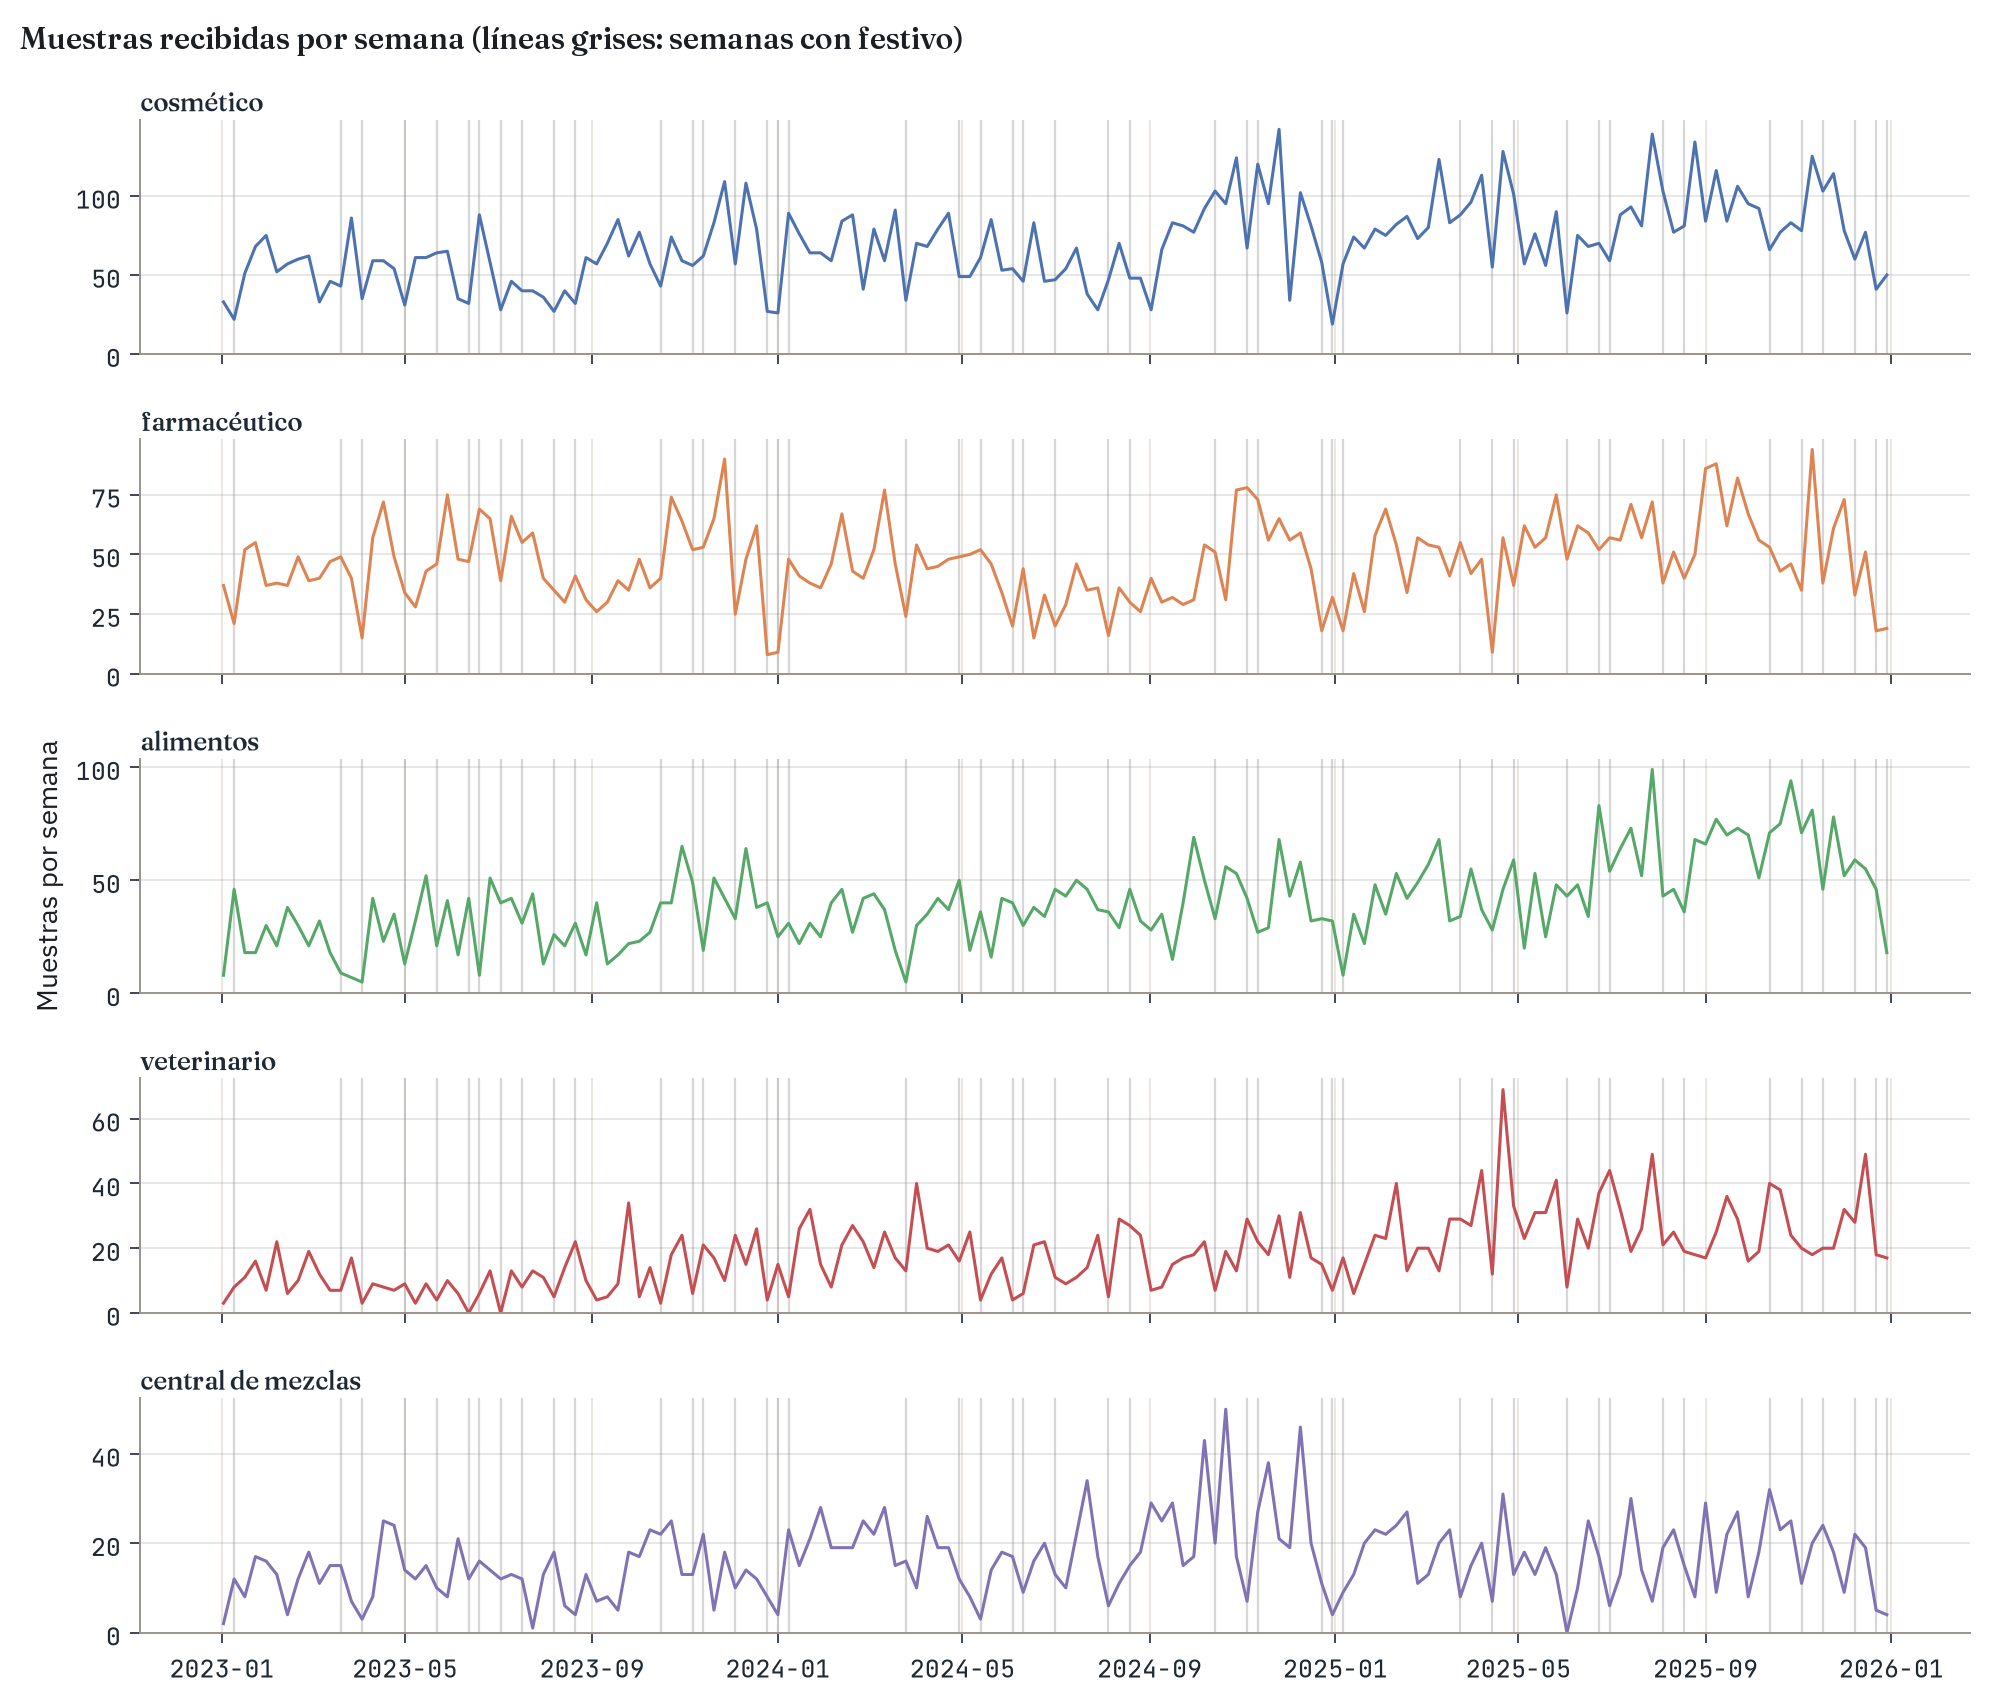
\includegraphics[width=0.7\textwidth]{02_volumen_semanal.png}
\caption{Muestras recibidas por semana en cada línea de negocio durante el
desarrollo. Conviene fijarse en las caídas que coinciden con las semanas con
festivo (líneas grises verticales) y en que las líneas no suben y bajan a la
vez: la carga total depende de la mezcla de clientes de cada día.}
\label{fig:volumen}
\end{figure}

\paragraph{Implicación.} La carga diaria tiene una parte predecible (día de la
semana, festivos, visitas de muestreo programadas y nivel reciente), lo que
justifica un análisis de regresión con variables de calendario y de
programación, siempre con validación temporal, porque la serie no es
estacionaria.

\subsection{No conformidad y sus factores}

Entre las muestras aceptadas del desarrollo, el \ExpTasaNoConformePct{}\,\%
resulta no conforme, es decir, hay unas \ExpConformesPorNoConforme{} conformes
por cada no conforme, y la tasa mensual oscila entre
\ExpTasaMensualMinPct{}\,\% y \ExpTasaMensualMaxPct{}\,\% (con
\ExpTasaPrimerAnioPct{}\,\% en \ExpPrimerAnio{} y \ExpTasaUltimoAnioPct{}\,\%
en \ExpUltimoAnio{}). La Figura~\ref{fig:tasas} muestra que la tasa cambia
según la línea de negocio, la matriz y el ensayo, y la
Figura~\ref{fig:transporte} que las condiciones de transporte importan sobre
todo en combinación: en el cuarto de muestras con transporte más largo la
tasa es de \ExpHorasCuartoAltoPct{}\,\%, frente a \ExpHorasCuartoBajoPct{}\,\%
en el más corto, y algo parecido ocurre con la temperatura
(\ExpTemperaturaCuartoAltoPct{}\,\% frente a \ExpTemperaturaCuartoBajoPct{}\,\%).

\begin{figure}[!htbp]
\centering
\begin{minipage}[t]{0.47\textwidth}\centering
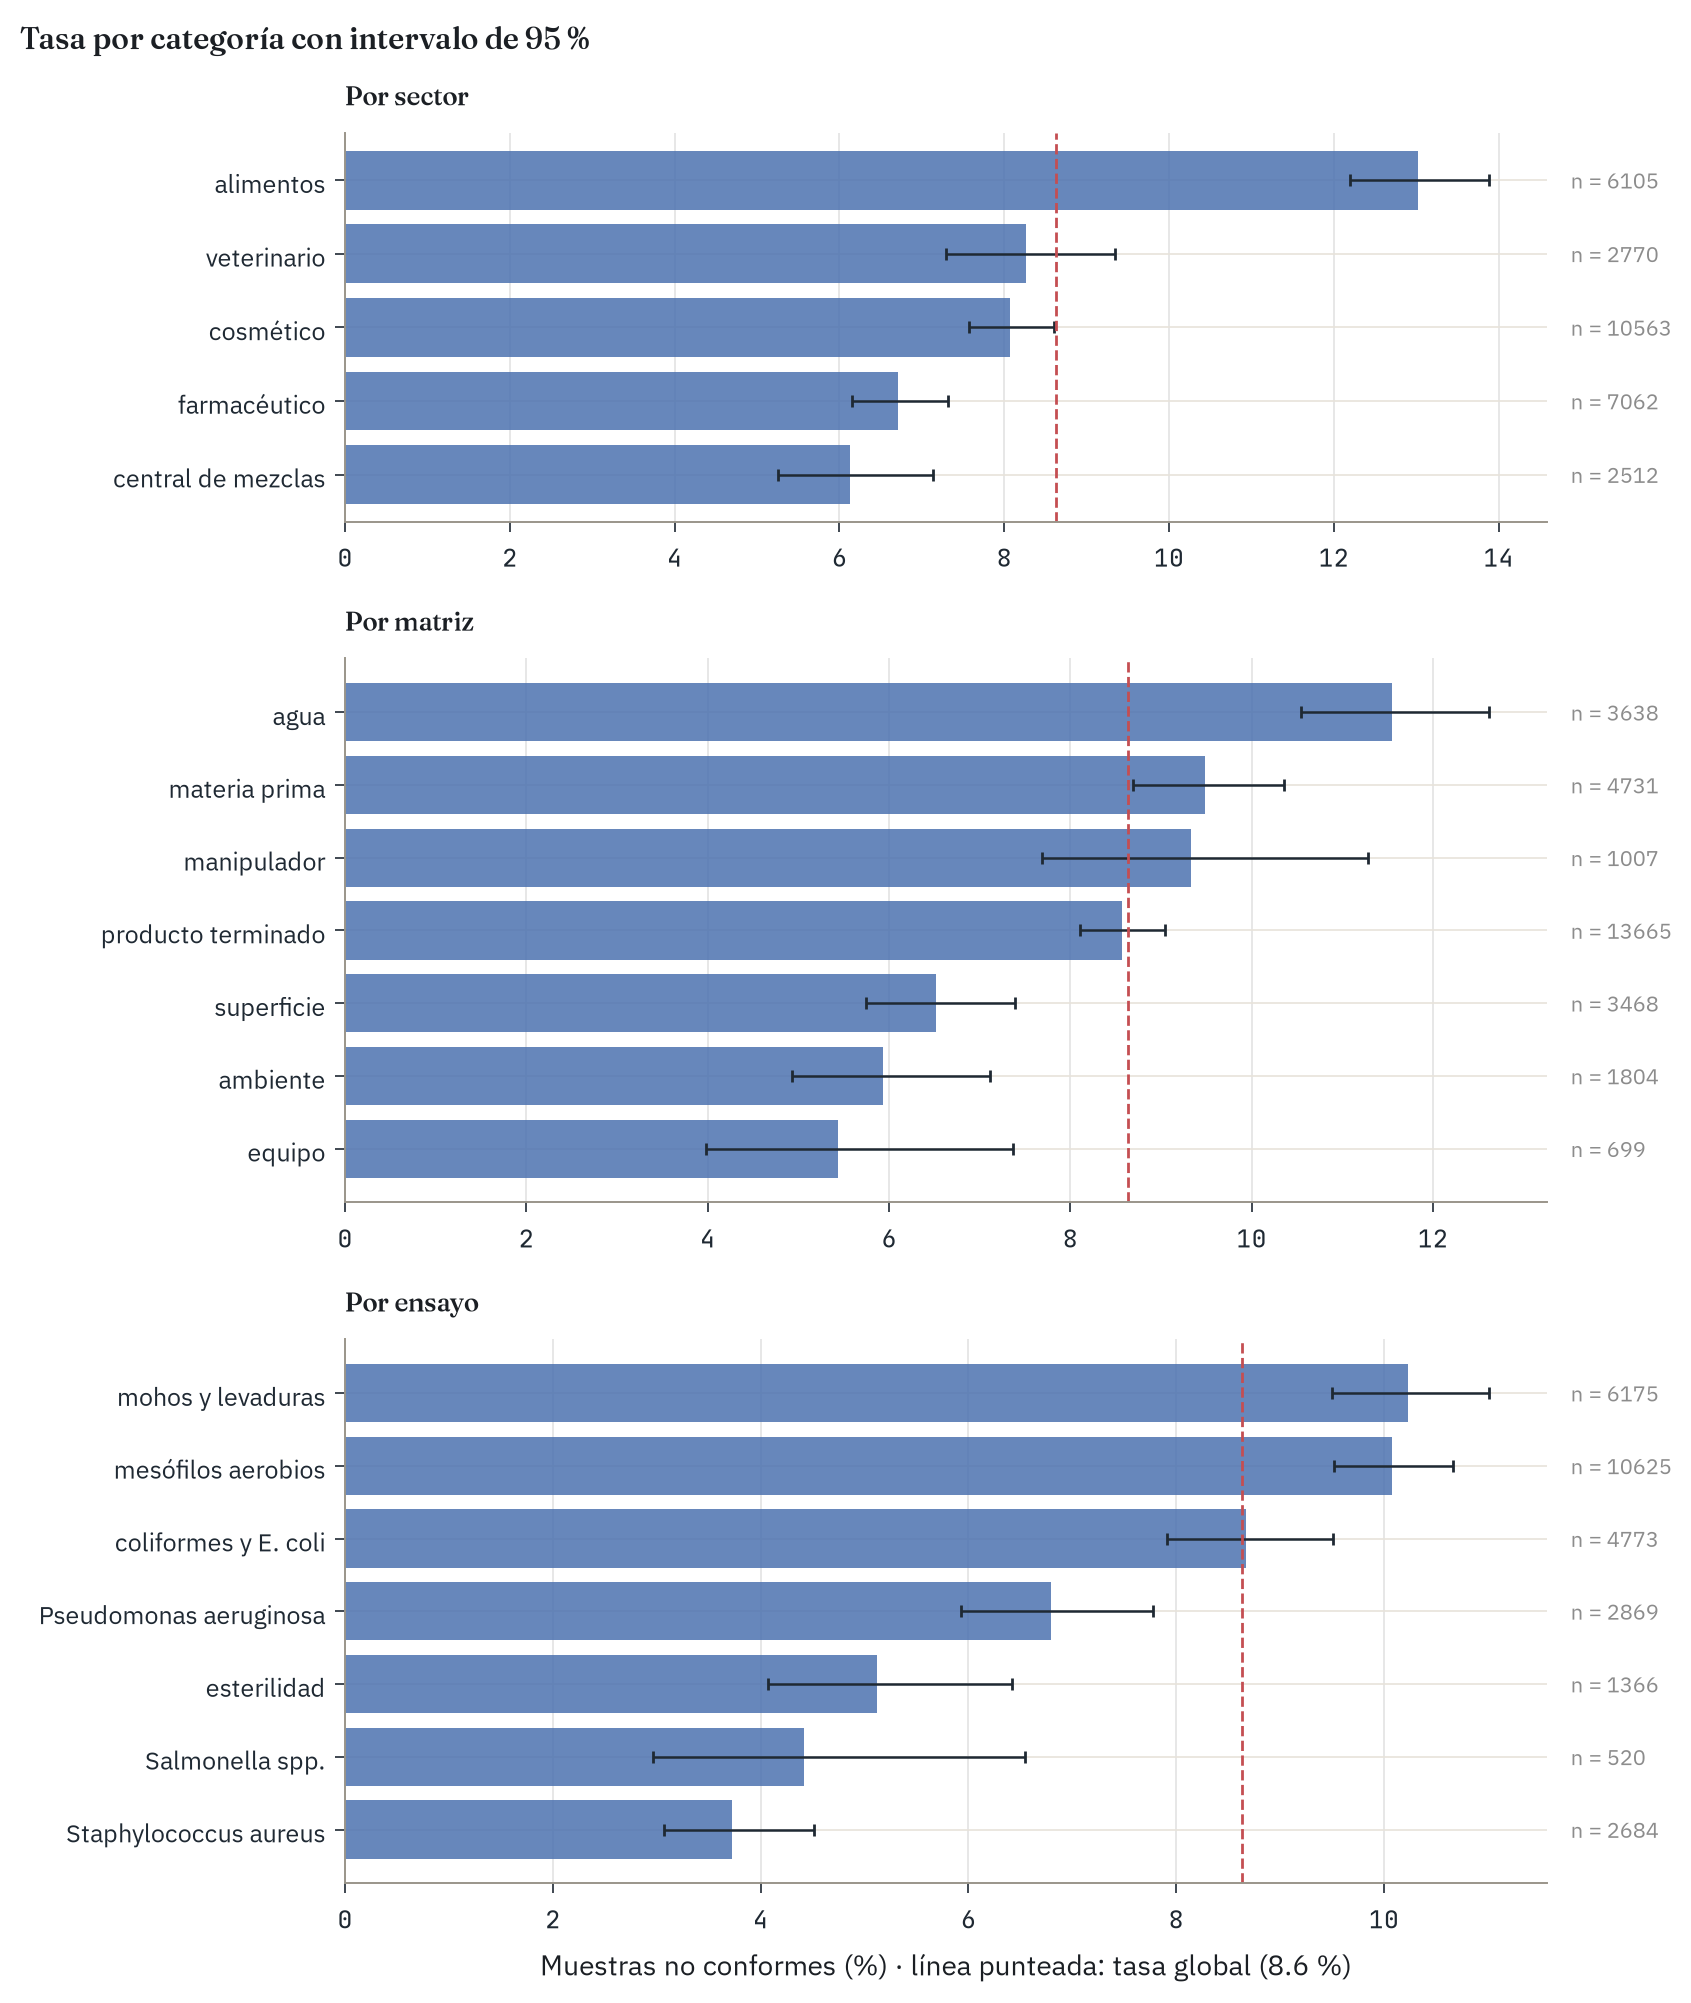
\includegraphics[width=\textwidth]{02_tasa_por_categoria.png}
\caption{Porcentaje de no conformes por línea de negocio, matriz y ensayo,
con intervalo de 95\,\%. La línea punteada es la tasa global; las barras
cuyo intervalo no la cruza son las categorías que de verdad se apartan.}
\label{fig:tasas}
\end{minipage}\hfill
\begin{minipage}[t]{0.49\textwidth}\centering
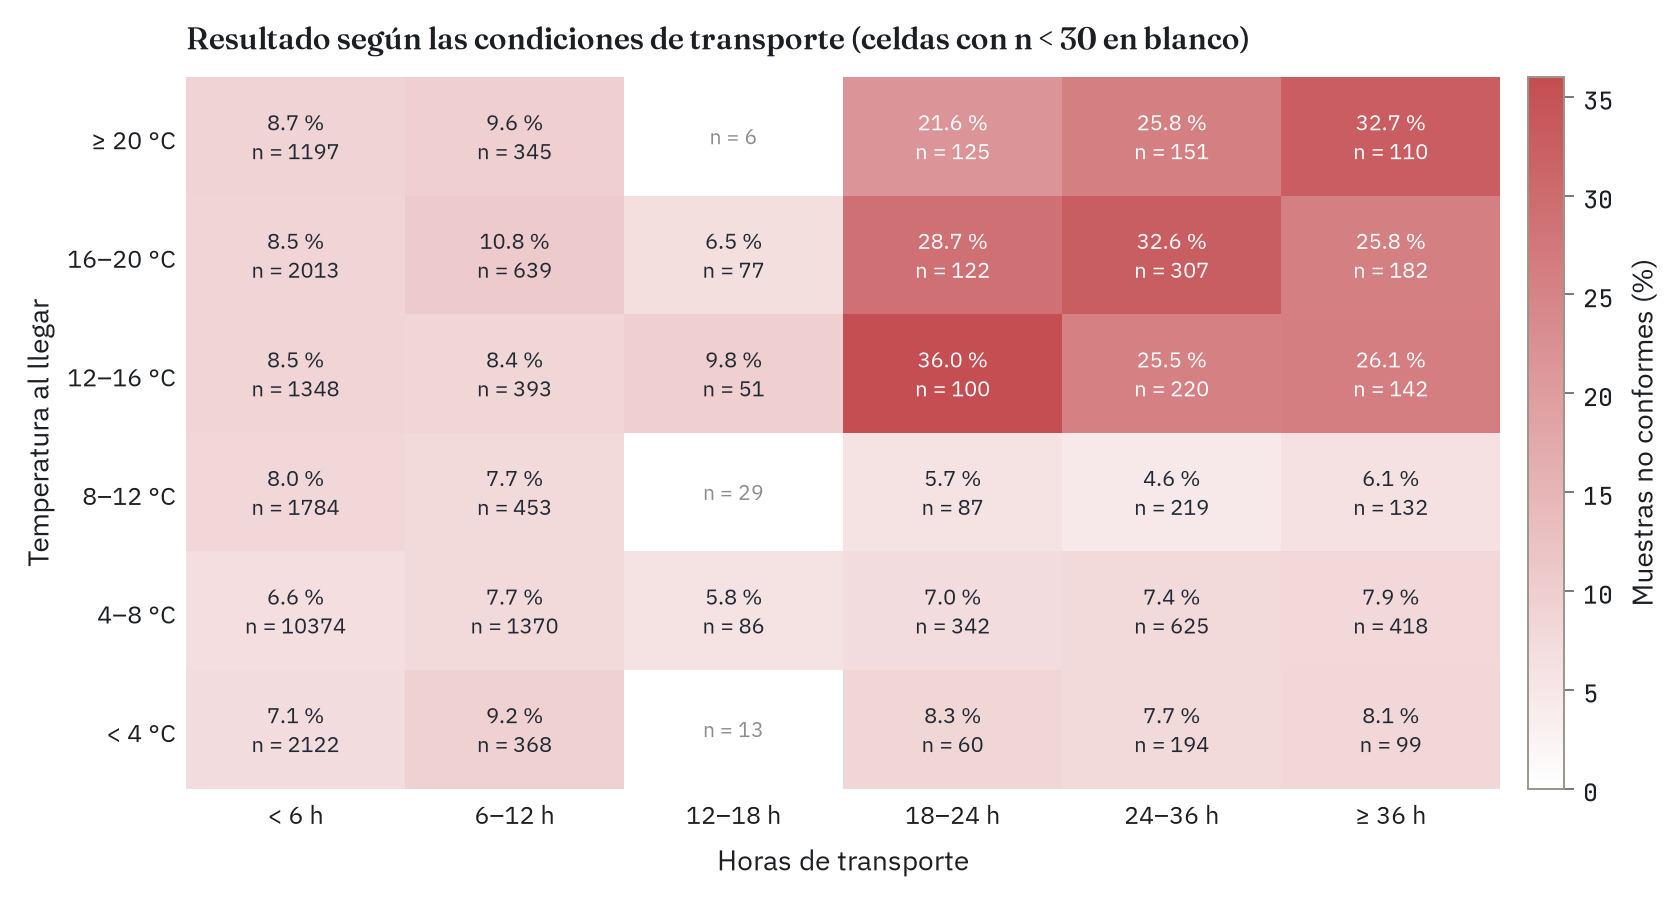
\includegraphics[width=\textwidth]{02_transporte.png}
\caption{Porcentaje de no conformes según horas y temperatura de transporte
(celdas con menos de 30 muestras en blanco). La tasa se dispara en la esquina
superior derecha, donde un transporte largo coincide con una temperatura
alta, y no a lo largo de una sola fila o columna.}
\label{fig:transporte}
\end{minipage}
\end{figure}

Individualmente, ninguna variable explica mucho, ya que la más correlacionada
con la no conformidad, \codigo{\ExpVariableCorrObjetivo}, tiene una
correlación de Spearman de apenas \ExpRhoObjetivo{}, y la variable de llegada
que más separa conformes de no conformes es \codigo{\ExpVariableMasSepara},
con una diferencia de medias de \ExpDiferenciaEstandarMax{} desviaciones
estándar. Entre las variables de entrada, el par más correlacionado
(\codigo{\ExpParCorrelacionado}) tiene $\rho$ de \ExpRhoPar{}, así que no hay
redundancias graves en las variables crudas. Por último, la categórica con
más niveles es \codigo{\ExpCategoriaMasNiveles}, con \ExpNivelesCategoria{}
niveles, y los informes tardan una mediana de \ExpEntregaMediana{} días
(percentil 90 de \ExpEntregaPNoventa{}), con un \ExpEntregaTardiaPct{}\,\%
entregado tarde.

\paragraph{Implicaciones.} Primeramente, el desbalance (una no conforme por
cada \ExpConformesPorNoConforme{} conformes) obliga a medir con ROC-AUC,
precisión media y costo, no con exactitud, y a probar el sobremuestreo como un
factor más. En segundo lugar, la señal es débil y repartida, de forma que se
esperan habilidades moderadas y conviene incluir variables derivadas que
capturen interacciones (como temperatura por horas de transporte) e
historiales recientes por cliente y producto. Finalmente, las categóricas con
muchos niveles exigen agrupar los niveles raros antes de codificar.

% =====================================================================
% metodologia.tex
% Responsabilidad única: describir la metodología común a los análisis
% (cribado con regla prerregistrada, protocolo temporal, diseño L16 de
% Taguchi y su contraste con el factorial completo, métricas, habilidad y
% costo de los errores). Cifras: macros Cri*, Dat*, Reg*, Clf*.
% =====================================================================
\section{Metodología}
\label{sec:metodologia}

\subsection{Cribado de análisis con una regla fijada de antemano}
\label{sec:cribado}

Con la misma base se pueden plantear muchas preguntas, y estudiar a fondo
todas habría diluido el trabajo, así que primeramente se armó un catálogo de
\CriCandidatos{} análisis candidatos (\CriCandidatosReg{} de regresión,
\CriCandidatosClf{} de clasificación, \CriCandidatosAgr{} de agrupamiento y
\CriCandidatosBayes{} bayesianos, estos últimos sin cribar porque no
compiten entre sí), cada uno con su objetivo, su unidad de análisis, su
momento de predicción y un valor de negocio de 1 a 3 asignado antes de ver
resultados. Para cada candidato se construyó una tabla de modelado
(\CriTablasConstruidas{} en total), y las \CriAuditoriasSuperadas{} superaron
la auditoría automática de fugas, que comprueba que ninguna variable tenga un
momento posterior al de la predicción.

Después, cada candidato pasa por la misma prueba rápida, solo con
entrenamiento y \DatBloquesCV{} bloques temporales, una línea base, un modelo
lineal o logístico y un árbol de profundidad \CriProfundidadArbol{}, todo sin
afinar (la prueba completa tomó \CriSegundosPrueba{} segundos). La regla de
selección, escrita en el código antes de mirar resultados y sin ajustes
posteriores, es la siguiente:

\begin{itemize}
    \item \textbf{Tamaño mínimo:} un supervisado necesita al menos
          \CriMinimoFilas{} filas de entrenamiento (y, si es de clasificación,
          \CriMinimoPositivos{} positivos), y un agrupamiento al menos
          \CriMinimoFilasAgrupamiento{} filas.
    \item \textbf{Estabilidad:} la habilidad frente a la línea base debe ser
          positiva en todos los bloques, no solo en promedio.
    \item \textbf{No basta una regla simple:} si un árbol que solo ve la mejor
          variable logra el \CriUmbralReglaSimplePct{}\,\% o más de la
          habilidad, el análisis no necesita un modelo y se descarta del
          estudio a fondo.
    \item \textbf{Tendencia a agruparse:} un agrupamiento necesita un
          estadístico de Hopkins mayor que \CriUmbralHopkins{}.
    \item \textbf{Puntaje:} habilidad media (o silueta) por valor de negocio
          dividido entre 3; en cada tipo gana el elegible de mayor puntaje.
\end{itemize}

\begin{figure}[!htbp]
\centering
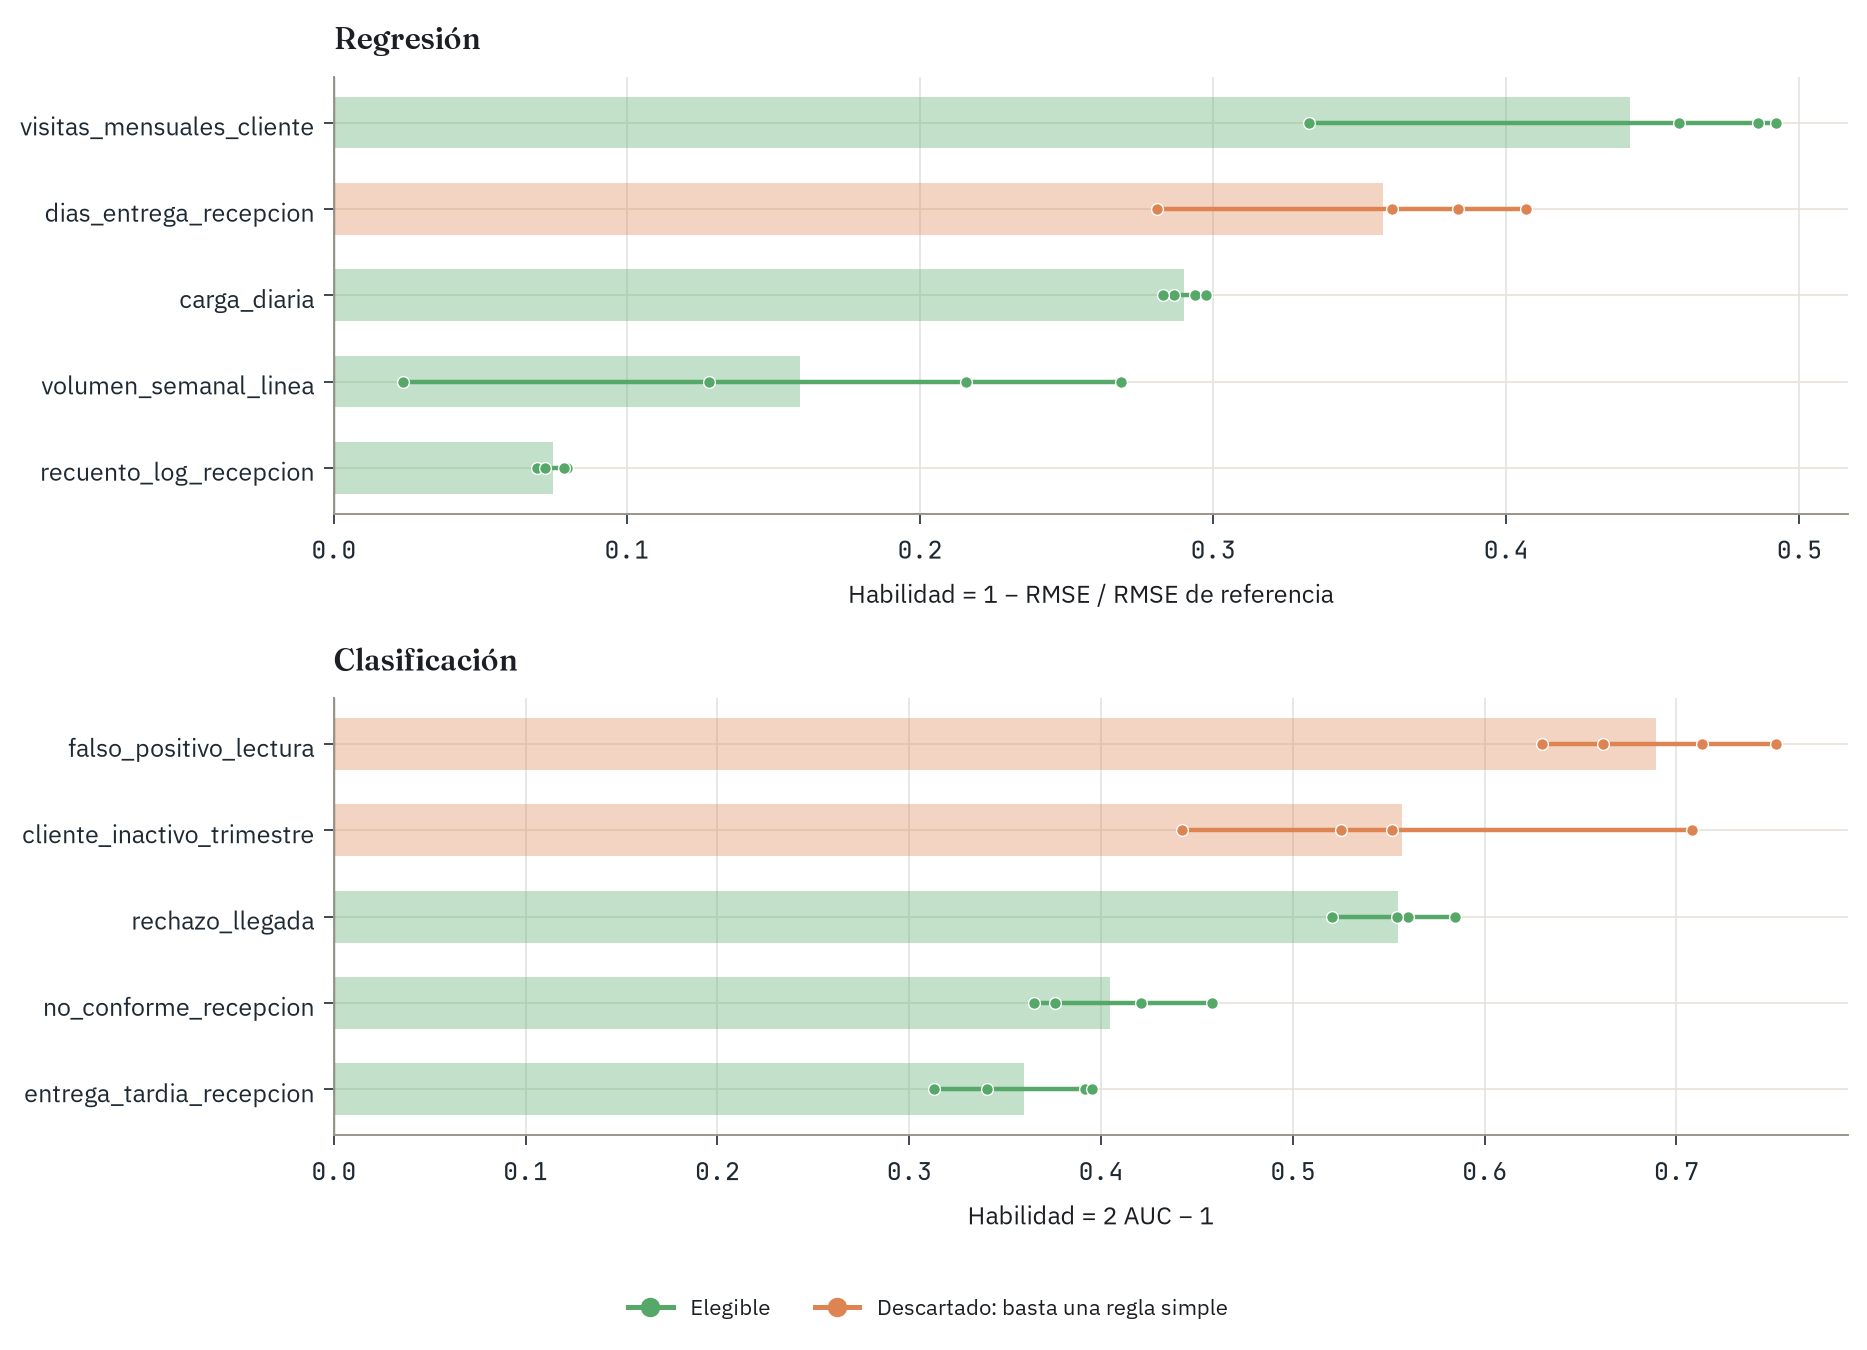
\includegraphics[width=0.66\textwidth]{03_habilidad.png}
\caption{Habilidad de cada supervisado en el cribado (barra: media; puntos:
cada bloque temporal). Los puntos muestran qué tan estable es la habilidad
entre bloques, y el color separa los elegibles de los descartados porque una
sola variable basta.}
\label{fig:cribado}
\end{figure}

De los \CriCribados{} candidatos cribados, \CriElegibles{} resultaron
elegibles, los \CriSupervisadosEstables{} supervisados superaron a su línea
base en todos los bloques y \CriDescartadosReglaSimple{} se descartaron porque
basta una regla simple (Figura~\ref{fig:cribado} y
Tablas~\ref{tab:cribado-reg} y~\ref{tab:cribado-clf}). El caso más ilustrativo
es \codigo{\CriClfMasHabil}, el clasificador con la mayor habilidad bruta
(\CriClfMasHabilHabilidad{}), del que la mejor variable sola logra el
\CriClfMasHabilProporcion{}\,\%, es decir, que en lugar de un modelo basta una
regla sobre el recuento, y esa regla es justamente la que se desarrolla en la
Sección~\ref{sec:bayes}. En regresión ocurre algo parecido con
\codigo{dias\_entrega\_recepcion}, que tiene más habilidad que el elegido pero
la explica casi entera el plazo prometido. El candidato más inestable,
\codigo{\CriMasInestable}, pasa de una habilidad de \CriMasInestableMin{} a
\CriMasInestableMax{} entre bloques.

\begin{table}[!htbp]
\centering
\tablaancha{cribado_regresion}
\caption{Cribado de los análisis de regresión (solo entrenamiento). La
habilidad es $1-\mathrm{RMSE}/\mathrm{RMSE}_\text{base}$ y la proporción de la
regla es la fracción de esa habilidad que logra la mejor variable sola.}
\label{tab:cribado-reg}
\end{table}

\begin{table}[!htbp]
\centering
\tablaancha{cribado_clasificacion}
\caption{Cribado de los análisis de clasificación (solo entrenamiento). La
habilidad es $2\cdot\mathrm{AUC}-1$; una proporción de la regla mayor que 1
indica que la variable sola supera al modelo.}
\label{tab:cribado-clf}
\end{table}

La regla eligió \codigo{\CriSeleccionReg} en regresión (habilidad
\CriSeleccionRegHabilidad{}, puntaje \CriSeleccionRegPuntaje{}),
\codigo{\CriSeleccionClf} en clasificación (ROC-AUC
\CriSeleccionClfAUC{}, puntaje \CriSeleccionClfPuntaje{}) y
\codigo{\CriSeleccionAgr} en agrupamiento (silueta
\CriSeleccionAgrSilueta{} con $k=\CriMejorSiluetaK$, Hopkins entre
\CriHopkinsMin{} y \CriHopkinsMax{} entre los candidatos). El agrupamiento
\codigo{\CriAgrComplementario} se estudia también, pero como análisis
complementario, fuera de la regla.

\subsection{Protocolo temporal}
\label{sec:protocolo}

Como los datos son una serie en el tiempo, la partición no es aleatoria sino
por fecha de recepción (Figura~\ref{fig:protocolo} y
Tabla~\ref{tab:particion}), de forma que todo modelo se evalúa siempre sobre
un periodo posterior al que vio. Dentro de entrenamiento, la validación
cruzada usa bloques de ventana creciente, y la partición de prueba solo puede
leerse a través de una función que existe en la etapa~07, la cual registra
cada lectura en un archivo que la verificación automática revisa.

% =====================================================================
% protocolo.tex
% Responsabilidad única: dibujar el protocolo temporal del proyecto
% (entrenamiento, validación y prueba por fechas; qué se hace con cada bloque;
% validación cruzada de ventana creciente y punto de congelamiento). Fechas y
% tamaños son macros generadas por los notebooks.
% =====================================================================
\begin{figure}[!htbp]
\centering
\begin{tikzpicture}[
    every node/.style={font=\small},
    caja/.style={draw, rounded corners=2pt, align=center, minimum height=1.05cm, inner sep=4pt},
    paso/.style={draw, rounded corners=2pt, align=center, fill=gray!6, text width=4.2cm,
                 minimum height=1.9cm, inner sep=4pt},
    flecha/.style={-{Stealth[length=2.2mm]}, thick},
]
% --- Datos y partición por fechas ------------------------------------------
\node[caja, fill=gray!10, text width=15.2cm] (datos) at (0,0)
    {\textbf{Datos:}\enspace \ExpMuestrasLimpias{} muestras limpias recibidas entre \DatDesde{} y \DatHasta{}\\[1pt]
     {\scriptsize\color{gray!70!black}partición por fecha de recepción, sin mezclar: Cortes en \DatCorteValidacion{} y \DatCortePrueba{}}};

\node[caja, fill=classblue!14, draw=classblue, text width=4.2cm] (tr) at (-5.3,-2.2)
    {\textbf{Entrenamiento}\\ antes de \DatCorteValidacion{}\\ \ExpFilasEntrenamiento{} muestras, \RegDiasEntrenamiento{} días};
\node[caja, fill=classgreen!16, draw=classgreen, text width=4.2cm] (val) at (0,-2.2)
    {\textbf{Validación}\\ \DatCorteValidacion{} a \DatCortePrueba{}\\ \ExpFilasValidacion{} muestras, \RegDiasValidacion{} días};
\node[caja, fill=classred!12, draw=classred, text width=4.2cm] (te) at (5.3,-2.2)
    {\textbf{Prueba}\\ desde \DatCortePrueba{}\\ \ExpFilasPrueba{} muestras, \FinDiasPrueba{} días};

\foreach \n in {tr, val, te} \draw[flecha, gray] (datos.south -| \n) -- (\n.north);

% --- Qué se hace con cada bloque ------------------------------------------
\node[paso, below=0.75cm of tr] (ajuste)
    {\textbf{Ajustar y explorar}\\ cribado, L16 de Taguchi y rejilla, con validación cruzada temporal};
\node[paso, below=0.75cm of val] (decidir)
    {\textbf{Decidir y congelar}\\ modelo, calibración y umbral por costo; Reajuste con entrenamiento + validación};
\node[paso, below=0.75cm of te] (evaluar)
    {\textbf{Evaluar una sola vez}\\ Etapa 07: Métricas con intervalos bootstrap, sin cambiar nada};

\draw[flecha, classblue] (tr) -- (ajuste);
\draw[flecha, classgreen] (val) -- (decidir);
\draw[flecha, classred] (te) -- (evaluar);
\draw[flecha] (ajuste) -- (decidir);
\draw[flecha] (decidir) -- (evaluar);

% --- Barrera de congelamiento ----------------------------------------------
\coordinate (barrera) at ($(te.west)+(-0.28,0)$);
\draw[classred, very thick, dashed] ($(barrera)+(0,0.9)$) -- ($(barrera |- evaluar.south)+(0,-0.1)$);
\node[classred, font=\scriptsize\bfseries, align=center, fill=white, inner sep=1pt]
    at ($(barrera)+(0,1.2)$) {lectura única y registrada};

% --- Validación cruzada de ventana creciente (dentro de entrenamiento) ------
\begin{scope}[shift={($(ajuste.south)+(-2.1,-0.55)$)}]
  \node[font=\scriptsize, anchor=west, gray!70!black] at (0,0)
      {\DatBloquesCV{} bloques de ventana creciente (solo entrenamiento):};
  \foreach \i/\a in {1/1.6, 2/2.3, 3/3.0, 4/3.7} {
    \fill[classblue!45] (0,-0.28*\i-0.12) rectangle (\a,-0.28*\i+0.04);
    \fill[classgreen!70] (\a,-0.28*\i-0.12) rectangle (\a+0.7,-0.28*\i+0.04);
  }
  \node[font=\scriptsize, anchor=west] at (4.6,-0.55) {\textcolor{classblue}{ajusta}};
  \node[font=\scriptsize, anchor=west] at (4.6,-0.9) {\textcolor{classgreen!70!black}{valida}};
\end{scope}
\end{tikzpicture}
\caption{Protocolo temporal del proyecto, donde cada bloque de fechas cumple
un solo papel: Con entrenamiento ajustamos y exploramos configuraciones con
validación cruzada de ventana creciente (abajo a la izquierda, donde cada
pliegue entrena con el pasado y valida con el tramo siguiente). Con
validación decidimos y congelamos. La prueba se abre una sola vez en la
etapa~07, que deja registrada cada lectura.}
\label{fig:protocolo}
\end{figure}


\begin{table}[!htbp]
\centering
\small
\tablagen{particion}
\caption{Muestras por bloque temporal (todas las muestras limpias, por fecha
de recepción). Cada análisis tiene su propia unidad, por ejemplo días hábiles
en la regresión, pero respeta los mismos cortes.}
\label{tab:particion}
\end{table}

\subsection{Diseño ortogonal L16 de Taguchi}
\label{sec:taguchi}

Para cada análisis elegido quedan seis decisiones de diseño, el modelo
(KNN, lineal o logístico, árbol o perceptrón multicapa, a cuatro niveles), el
escalado (estándar o min-max), el grupo de variables (base o ampliado), la
selección de variables por $F$ (ninguna o las $k$ mejores), la codificación
de categóricas (one-hot u ordinal) y un sexto factor propio de cada tarea
(objetivo en logaritmo en la regresión, sobremuestreo de la clase minoritaria
en la clasificación). El factorial completo tiene
$4\times 2^5=\RegCorridasCompleto$ combinaciones, y en lugar de correrlas
todas se usa un arreglo ortogonal L16, que con 16 corridas mantiene cada par
de factores balanceado.

\paragraph{Estructura de alias.} El factor de cuatro niveles ocupa tres
columnas del arreglo (dos columnas base y su interacción), el escalado otra,
y los cuatro factores restantes columnas generadas por productos, de forma
que tres columnas (\codigo{ac}, \codigo{bc} y \codigo{abc}) quedan libres para
estimar la interacción modelo $\times$ escalado, la que más se esperaba (KNN y
el perceptrón dependen de la escala, el árbol no). De las
\RegInteracciones{} interacciones de dos factores, \RegInteraccionesLibres{}
quedan libres de confusión con un efecto principal; las demás comparten
columna con otro efecto y por eso el método supone, y luego comprueba con una
corrida de confirmación, que no son grandes.

\paragraph{Razón señal/ruido.} Cada corrida se evalúa en los
\DatBloquesCV{} bloques temporales, y sus puntajes $y_1,\dots,y_n$ se
resumen en una razón señal/ruido (S/N, en dB) que premia a la vez el buen
promedio y la poca variación entre bloques:
\[
\text{S/N}_\text{menor} = -10\log_{10}\Bigl(\tfrac{1}{n}\textstyle\sum_i y_i^2\Bigr)
\quad\text{(RMSE)},\qquad
\text{S/N}_\text{mayor} = -10\log_{10}\Bigl(\tfrac{1}{n}\textstyle\sum_i y_i^{-2}\Bigr)
\quad\text{(ROC-AUC)}.
\]
Con las 16 corridas se construye la tabla de respuesta (S/N medio de cada
nivel, delta entre el mejor y el peor nivel y rango de cada factor), y el
modelo aditivo predice la S/N de la combinación de mejores niveles. Esa
combinación se corre de verdad (corrida de confirmación) y, si la S/N
observada cae dentro de una tolerancia de la predicha, se acepta que las
interacciones no rompen el modelo aditivo. Finalmente, la mejor configuración
(confirmación o mejor corrida observada) pasa a una búsqueda en rejilla de
sus hiperparámetros con los mismos bloques temporales.

\paragraph{Contraste con el factorial completo.} En la regresión, donde cada
corrida es barata, se corrió además el factorial completo
(\RegCorridasCompleto{} corridas, \RegSegundosCompleto{} segundos frente a
\RegSegundosLSixteen{} del L16) para comprobar si el atajo cambia las
conclusiones. La correlación de Spearman entre los deltas de ambos diseños es
de \RegRhoCompleto{}, \RegFactoresMismoOptimo{} de los \RegFactores{} factores
tienen el mismo mejor nivel en ambos, y el orden de los dos factores más
influyentes, modelo y grupo, se conserva (Figura~\ref{fig:l16-completo}). La
mejor S/N del factorial completo (\RegSNMejorCompleto{} dB) es apenas mayor
que la mejor corrida del L16 (\RegSNMejorCorrida{} dB), y la confirmación
quedó en el puesto \RegPuestoConfirmacion{} de las \RegCorridasCompleto{}
combinaciones. En la clasificación el factorial completo no se corrió (se
estimaron \ClfSegundosCompletoEstimados{} segundos, frente a
\ClfSegundosLSixteen{} del L16), y por eso allí la corrida de confirmación es
la única comprobación del modelo aditivo.

\begin{figure}[!htbp]
\centering
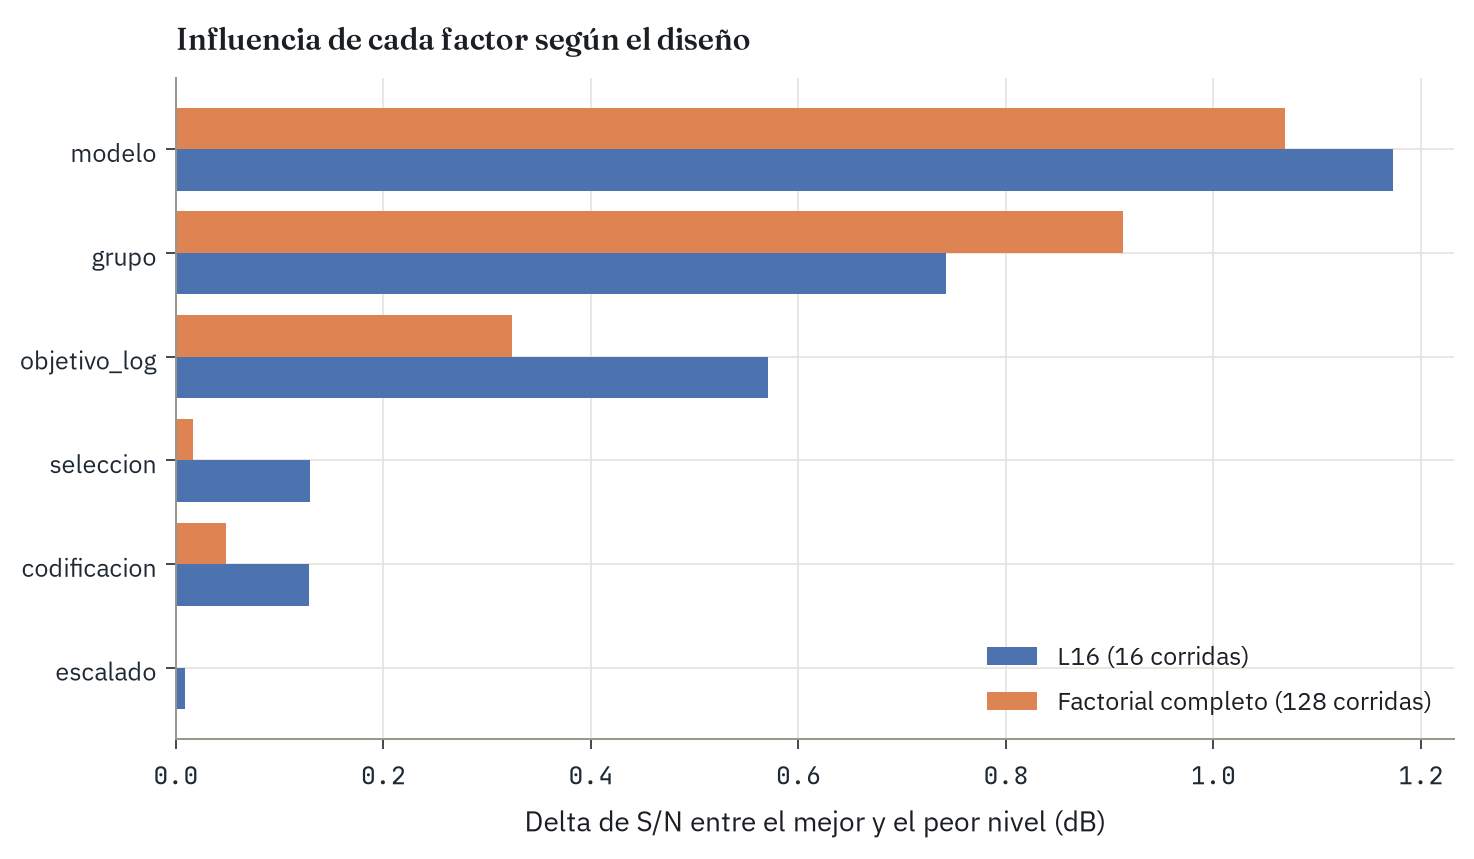
\includegraphics[width=0.5\textwidth]{04_l16_contra_completo.png}
\caption{Delta de S/N de cada factor de la regresión según el L16 (azul) y
el factorial completo (naranja). Lo que importa es que el orden de los
factores y la separación entre los influyentes (modelo, grupo, objetivo en
logaritmo) y los despreciables (escalado) se mantiene con una octava parte de
las corridas.}
\label{fig:l16-completo}
\end{figure}

\subsection{Métricas, habilidad y costo de los errores}
\label{sec:metricas}

Las métricas siguen los temas del curso \cite{muller2016,hastie2009}, con dos
añadidos para que las cifras se puedan comparar entre análisis:

\begin{itemize}
    \item \textbf{Regresión:} MAE, RMSE y $R^2$. La \emph{habilidad} es
          $1-\mathrm{RMSE}/\mathrm{RMSE}_\text{ref}$, donde la referencia es la
          mejor regla ingenua, por ejemplo la media de los cinco días
          hábiles anteriores (\codigo{base\_media\_5}); una habilidad de cero
          significa no mejorar lo que ya se haría sin modelo.
    \item \textbf{Clasificación:} ROC-AUC, precisión media (área bajo la curva
          de precisión y recall, más exigente con el desbalance) y puntaje de
          Brier (error cuadrático de la probabilidad, que mide calibración). La
          habilidad es $2\cdot\mathrm{AUC}-1$, que vale cero para un
          clasificador al azar.
    \item \textbf{Incertidumbre:} las métricas de validación y prueba llevan
          intervalos bootstrap de 95\,\%, y las proporciones (por ejemplo,
          reensayos conformes) intervalos de Wilson.
\end{itemize}

\paragraph{Costo de los errores.} En la clasificación, dejar pasar una muestra
no conforme sin alerta (falso negativo) cuesta \DatCostoFN{} veces lo que
revisar una que resulta conforme (falso positivo, costo \DatCostoFP{}), de
forma que el costo total es
$L=C_\text{FP}\cdot\text{FP}+C_\text{FN}\cdot\text{FN}$. Si las
probabilidades están calibradas, el umbral que minimiza el costo esperado es
$t^\ast=C_\text{FP}/(C_\text{FP}+C_\text{FN})$, que aquí vale
\ClfUmbralTeorico{}; el umbral se elige en validación y se compara con ese
valor teórico. Como un costo bajo puede esconder una avalancha de falsas
alarmas, junto al costo se reportan siempre la precisión y las alertas por
semana.

% =====================================================================
% regresion.tex
% Responsabilidad única: presentar el análisis de regresión de la carga
% diaria (modelos del curso, Taguchi, rejilla, validación y modelo
% congelado). Cifras: macros Reg*; tablas tabla_reg_*; figuras 04_*.
% =====================================================================
\section{Regresión: carga diaria}
\label{sec:regresion}

El análisis \codigo{\RegAnalisis} predice \codigo{\RegObjetivo}, el número de
muestras que se reciben en un día hábil, con la información disponible en el
momento \codigo{\RegMomento}, es decir, el calendario (día de la semana,
festivos, cierre de mes), los puntos de muestreo programados para ese día y
el nivel reciente de la serie (rezagos y medias móviles). En entrenamiento hay
\RegDiasEntrenamiento{} días hábiles, con una media de
\RegMediaEntrenamiento{} muestras por día y un rango observado de
\RegMinimoEntrenamiento{} a \RegMaximoEntrenamiento{}.

\subsection{Pasada didáctica con los modelos del curso}

Primeramente se recorren los modelos del curso con una configuración
razonable y sin afinar, evaluados en los \RegBloques{} bloques temporales
(Tabla~\ref{tab:reg-didactica}). La regresión lineal simple usa la variable
más correlacionada con el objetivo, \codigo{\RegVariableSimple}
(correlación de Pearson de \RegCorrSimple{}), y su pendiente de
\RegPendienteSimple{} se lee como cuántas muestras más llegan, en promedio,
por cada punto de muestreo adicional programado; con un $R^2$ de
\RegRDosSimple{} en entrenamiento, esa sola variable deja sin explicar la
mayor parte de la variación, lo que motiva pasar a la regresión múltiple.

\begin{table}[!htbp]
\centering
\tablaancha{reg_didactica}
\caption{Pasada didáctica de regresión: media y desviación entre bloques. Las
tres primeras filas son referencias sin modelo; la habilidad se mide frente a
\codigo{base\_media\_5}, la mejor de ellas.}
\label{tab:reg-didactica}
\end{table}

La regresión lineal múltiple resultó el mejor modelo de esta pasada, con un
RMSE medio de \RegRMSELinealDidactico{} frente a \RegRMSEMLPDidactico{} del
perceptrón multicapa, y una habilidad de \RegHabilidadMejorDidactico{} cuyo
mínimo por bloque (\RegHabilidadMinMejorDidactico{}) casi no se aleja de la
media. La mejor referencia ingenua, \codigo{\RegMejorReferencia}, tiene un
RMSE medio de \RegRMSEReferencia{} (entre \RegRMSEReferenciaMin{} y
\RegRMSEReferenciaMax{} según el bloque), y los \RegDidacticosEstables{}
modelos didácticos la superan en todos los bloques. El árbol sin poda
(\RegHojasSinPoda{} hojas) se sobreajusta, con un RMSE medio de
\RegRMSESinPoda{}, y la poda por complejidad de costo con
$\alpha=\RegAlfaPoda$ lo reduce a \RegHojasPodado{} hojas y a un RMSE de
\RegRMSEPodado{}, mejor pero aún lejos de los modelos lineales, lo cual
sugiere que la relación es en buena parte aditiva.

En la regresión múltiple, el coeficiente estandarizado de mayor tamaño es el
de \codigo{\RegCoefPrincipal} (\RegCoefPrincipalValor{} muestras por
desviación estándar), seguido por la media móvil de
veinte días y el día de la semana. Las medias móviles de cinco y de veinte
días (\codigo{\RegParRedundante}) tienen una correlación de
\RegCorrParRedundante{}, así que sus coeficientes individuales deben leerse
con cautela, porque el modelo puede repartir entre ellas el mismo efecto.

\subsection{Taguchi y búsqueda en rejilla}

El L16 confirmó lo que sugería la pasada didáctica, el factor más influyente
es el \RegFactorPrincipal{} (delta de \RegDeltaPrincipal{} dB), seguido del
\RegFactorSegundo{} de variables (\RegDeltaSegundo{} dB), mientras que el
escalado es prácticamente indiferente (Tabla~\ref{tab:reg-respuesta}). El óptimo aditivo es
\emph{\RegOptimo}, con una S/N predicha de \RegSNPredicha{} dB y una
observada en la confirmación de \RegSNObservada{} dB, dentro de la
tolerancia de \RegToleranciaSN{} dB, de forma que se acepta el modelo aditivo.

\begin{table}[!htbp]
\centering
\small
\tablagen{reg_respuesta}
\caption{Tabla de respuesta de Taguchi para la regresión (S/N en dB; mayor es
mejor). El rango ordena los factores por su delta.}
\label{tab:reg-respuesta}
\end{table}

Aun así, la confirmación tuvo un RMSE medio de \RegRMSEConfirmacion{},
ligeramente peor que el de la mejor corrida observada (la corrida
\RegMejorCorrida{}, con \RegRMSEMejorCorrida{}), así que la configuración que
pasa a la rejilla sale de la \RegOrigenConfiguracion{}. La búsqueda en
rejilla con los mismos bloques dejó a la regresión lineal
(\RegRejillaLinealRMSE{}) por delante del perceptrón (\RegRejillaMLPRMSE{}),
sin hiperparámetros que afinar (\RegHiperparametros{}), y la elección final
no dependió de la regla de empate (tolerancia de \RegToleranciaEmpatePct{}\,\%,
empate: \RegPorEmpate{}). La configuración congelada es \emph{\RegConfiguracionFinal}.

\subsection{Validación y modelo congelado}

En validación, la regresión lineal obtuvo un RMSE de \RegRMSEValidacion{}
(IC 95\,\% de \RegRMSEValidacionInf{} a \RegRMSEValidacionSup{}), un MAE de
\RegMAEValidacion{}, un $R^2$ de \RegRDosValidacion{} y una habilidad de
\RegHabilidadValidacion{} (de \RegHabilidadValidacionInf{} a
\RegHabilidadValidacionSup{}), frente a un RMSE de \RegRMSEValidacionOtro{}
del \RegModeloOtro{}. La habilidad es algo
menor que la del cribado, y una razón visible es que el nivel de la serie
cambió, ya que la media sube de \RegMediaEntrenamiento{} muestras por día en
entrenamiento a \RegMediaValidacion{} en validación, y el residuo medio
(observado menos predicho) es de \RegResiduoMedioValidacion{}, es decir, el
modelo se queda ligeramente corto. La correlación entre la predicción y el
error absoluto es de \RegCorrResiduo{}, así que el error no crece de forma
marcada con la carga.

\begin{figure}[!htbp]
\centering
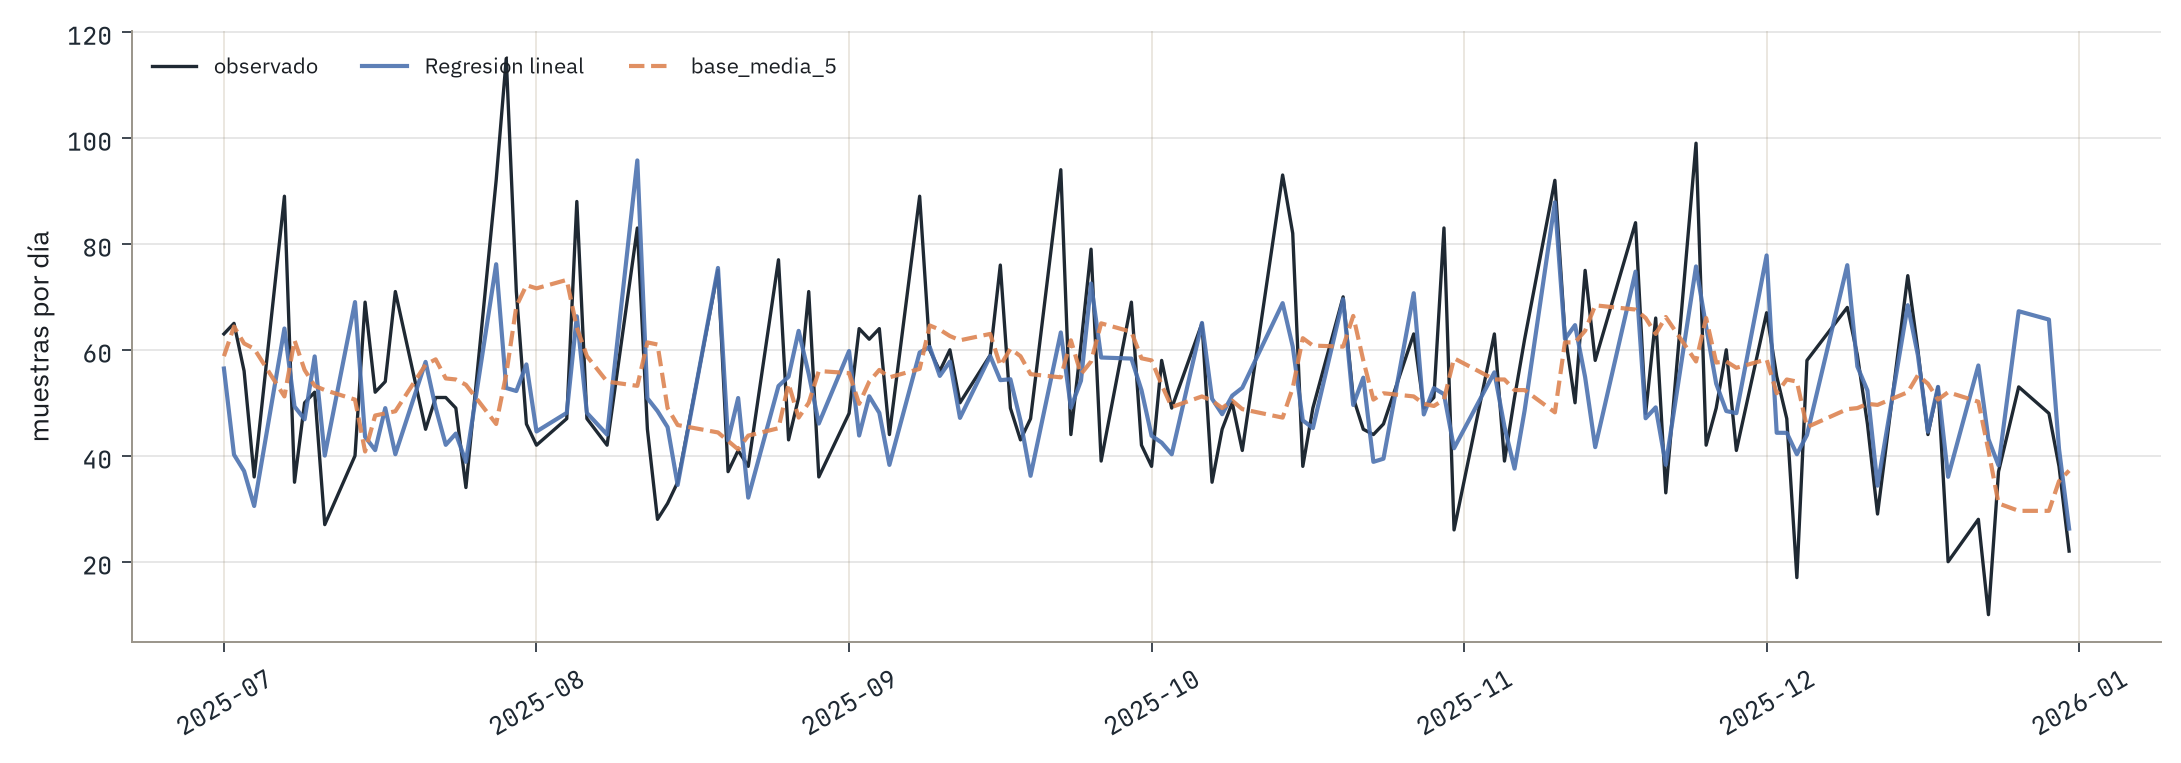
\includegraphics[width=0.85\textwidth]{04_validacion_serie.png}
\caption{Serie de validación: observado (negro), regresión lineal (azul) y
media de los cinco días anteriores (naranja). El modelo sigue los altibajos de
un día a otro, que la referencia solo suaviza, pero no alcanza los picos
aislados.}
\label{fig:reg-serie}
\end{figure}

\paragraph{Lectura operativa.} Si se acepta como tolerancia práctica un error
del \RegToleranciaOperativaPct{}\,\% de la media diaria (unas
\RegToleranciaOperativa{} muestras), el modelo queda fuera de ella en el
\RegDiasFueraPct{}\,\% de los días de validación, frente al
\RegDiasFueraReferenciaPct{}\,\% de la referencia, y su error absoluto medio es
de \RegMAEOperacion{} muestras frente a \RegMAEReferencia{}. Es una mejora
clara pero modesta, útil para planear turnos, no para fijar cupos exactos.
Finalmente, el modelo congelado (\RegModeloFinal{}, \RegVariablesModelo{}
variables tras codificar) se reajusta con entrenamiento más validación
(\RegFilasReajuste{} días) antes de abrir la prueba.

% =====================================================================
% clasificacion.tex
% Responsabilidad única: presentar el análisis de clasificación del riesgo
% de no conformidad (modelos del curso, Taguchi, sobremuestreo,
% calibración y umbral por costo con alertas por semana).
% Cifras: macros Clf*; tablas tabla_clf_*; figuras 05_*.
% =====================================================================
\section{Clasificación: Riesgo de no conformidad}
\label{sec:clasificacion}

La segunda pregunta sigue los mismos tres niveles de la regresión, pero aquí
aparecen dos problemas que allá no estaban. Hay pocas no conformes y eso
obliga a pensar en el sobremuestreo. Además la salida tiene que ser una
probabilidad que se pueda creer porque de ella dependen el umbral de alerta
y la capa bayesiana de la Sección~\ref{sec:bayes}.

El análisis \codigo{\ClfAnalisis} estima en el momento \codigo{\ClfMomento}
la probabilidad de que una muestra aceptada resulte no conforme
(\codigo{\ClfObjetivo}), con lo que se sabe al recibirla: El cliente y su
historial reciente, el producto y su matriz, el ensayo, las condiciones de
transporte y el calendario. En entrenamiento hay
\ClfMuestrasEntrenamiento{} muestras con \ClfPositivosEntrenamiento{} no
conformes (\ClfPrevalenciaEntrenamientoPct{}\,\%) y en validación
\ClfMuestrasValidacion{} con \ClfPositivosValidacion{}
(\ClfPrevalenciaValidacionPct{}\,\%).

\subsection{Pasada didáctica con los modelos del curso}

En la pasada didáctica (Tabla~\ref{tab:clf-didactica}) el mejor modelo fue la
\MakeLowercase{\ClfMejorDidactico}, con un ROC-AUC medio de
\ClfAUCMejorDidactico{} y una desviación de \ClfAUCDesvMejorDidactico{} entre
bloques. Su precisión media fue de \ClfPrecisionMediaMejorDidactico{} frente a
\ClfDummyPrecisionMedia{} del clasificador que solo predice la proporción de
no conformes, o sea que el modelo sí encuentra no conformes bastante por
encima de lo que daría el azar. El perceptrón multicapa quedó cerca
(\ClfAUCMLPDidactico{}) y el más débil fue \ClfPeorDidactico{}
(\ClfAUCPeorDidactico{}). Una explicación posible es que con decenas de
columnas codificadas todas las muestras quedan casi igual de lejos entre sí y
la distancia deja de distinguir a los vecinos.

\begin{table}[!htbp]
\centering
\tablaancha{clf_didactica}
\caption{Pasada didáctica de clasificación con la media y la desviación entre
bloques temporales: La habilidad es $2\,\mathrm{AUC}-1$ y la regresión
logística tiene el mayor ROC-AUC medio.}
\label{tab:clf-didactica}
\end{table}

El árbol sin poda crece hasta \ClfHojasSinPoda{} hojas y obtiene un ROC-AUC de
\ClfAUCSinPoda{}, mientras que la poda con $\alpha=\ClfAlfaPoda$ lo deja en
\ClfHojasPodado{} hojas con \ClfAUCPodado{}, es decir que quedó más simple y
mejor. Su hoja de mayor riesgo reúne \ClfHojaRiesgoFilas{} muestras con una
fracción de no conformes de \ClfHojaRiesgoFraccion{}, unas
\ClfHojaRiesgoVeces{} veces la tasa general. Las reglas de sus hojas más
riesgosas combinan el historial de no conformidad del producto con la
temperatura por las horas de transporte, que es la misma interacción que vimos
en la Figura~\ref{fig:transporte}.

En la regresión logística la variable que más sube el riesgo es
\codigo{\ClfVariableSube}, con una razón de odds de \ClfOddsSube{} (con las
demás variables fijas, sus odds de salir no conforme son unas
\ClfOddsSube{} veces las del resto) y la que más lo baja es
\codigo{\ClfVariableBaja} (\ClfOddsBaja{}). Estas razones solo valen para los
datos simulados porque esas relaciones las fijó el generador.

\paragraph{Efecto del sobremuestreo.} Sospechábamos que el sobremuestreo no le
pega igual a todos los modelos así que repetimos cada modelo de la pasada
con sobremuestreo de la clase minoritaria dentro de la tubería, sin tocar los
pliegues de validación (Tabla~\ref{tab:clf-sobre}). A la
\MakeLowercase{\ClfSobreMenosPierde} casi no le cambia el ROC-AUC
(\ClfSobreDeltaAUCMenor{}), pero al \MakeLowercase{\ClfSobreMasPierde} le
quita \ClfSobreDeltaAUC{}, algo que retomamos en la
Sección~\ref{sec:redes}. Lo más importante es que en todos los modelos el
puntaje de Brier empeora y la probabilidad media predicha se dispara. Es la
descalibración que esperábamos: El modelo aprende con una proporción de no
conformes que no es la real y aunque el orden de las muestras cambie poco sus
cifras dejan de ser probabilidades así que no podrían alimentar la capa
bayesiana sin recalibrarse.

\begin{table}[!htbp]
\centering
\tablacompacta{clf_sobremuestreo}
\caption{Modelos didácticos sin y con sobremuestreo: El ROC-AUC cambia poco
salvo en el perceptrón, pero el Brier y la probabilidad media muestran que el
sobremuestreo descalibra las probabilidades de todos.}
\label{tab:clf-sobre}
\end{table}

\subsection{Taguchi y búsqueda en rejilla}

En el L16 de clasificación el factor más influyente vuelve a ser el
\ClfFactorPrincipal{} (delta de \ClfDeltaPrincipal{} dB), seguido del
\ClfFactorSegundo{} (\ClfDeltaSegundo{} dB) y el escalado vuelve a ser
indiferente. El óptimo aditivo es \emph{\ClfOptimo}, con una S/N predicha de
\ClfSNPredicha{} dB (que equivale a un ROC-AUC de
\ClfAUCEquivalentePredicha{}). En la confirmación observamos \ClfSNObservada{}
dB (ROC-AUC de \ClfAUCConfirmacion{}), dentro de la tolerancia de
\ClfToleranciaSN{} dB. Como la confirmación superó a la mejor corrida
observada (la \ClfMejorCorrida{}, con \ClfSNMejorCorrida{} dB y ROC-AUC de
\ClfAUCMejorCorrida{}), a la rejilla pasó la configuración de la
\ClfOrigenConfiguracion{}.

Ese óptimo incluye el sobremuestreo, que en el promedio del L16 sube un poco
la S/N aunque en la logística de la pasada casi no movió el ROC-AUC. Como ya
sabíamos que descalibra lo dejamos con la condición de calibrar después. En la rejilla la logística
(\ClfRejillaLogisticaAUC{}) quedó por delante del árbol
(\ClfRejillaArbolAUC{}) con \ClfHiperparametros{} y un ROC-AUC por bloque de
\ClfAUCRejillaFinal{}, sin necesidad de la regla de empate
(\ClfPorEmpate{}).

\subsection{Validación y calibración}

En validación la logística ordenó mejor que el árbol, con un ROC-AUC de
\ClfAUCValidacionSinCalibrar{} antes de calibrar frente a
\ClfAUCValidacionOtro{} del \MakeLowercase{\ClfModeloOtro}. Sin embargo su
Brier sin calibrar (\ClfBrierSinCalibrar{}) es peor que el del clasificador
constante (\ClfDummyBrier{}), lo que confirma la descalibración que mete el
sobremuestreo. Por eso le ajustamos una calibración sigmoide con los bloques
temporales de entrenamiento, que es una curva en forma de S que convierte el
puntaje del modelo en una probabilidad que se parece a la frecuencia real.
Con ella el Brier baja a \ClfBrierCalibrado{} y la probabilidad media pasa
de \ClfProbMediaSinCalibrar{} a \ClfProbMediaCalibrado{}, cerca de la tasa
real, mientras que el orden casi no cambia. El ROC-AUC calibrado es de
\ClfAUCCalibrado{} (IC 95\,\% de \ClfAUCValidacionInf{} a
\ClfAUCValidacionSup{}) y la precisión media de \ClfPrecisionMediaValidacion{}.

\begin{figure}[!htbp]
\centering
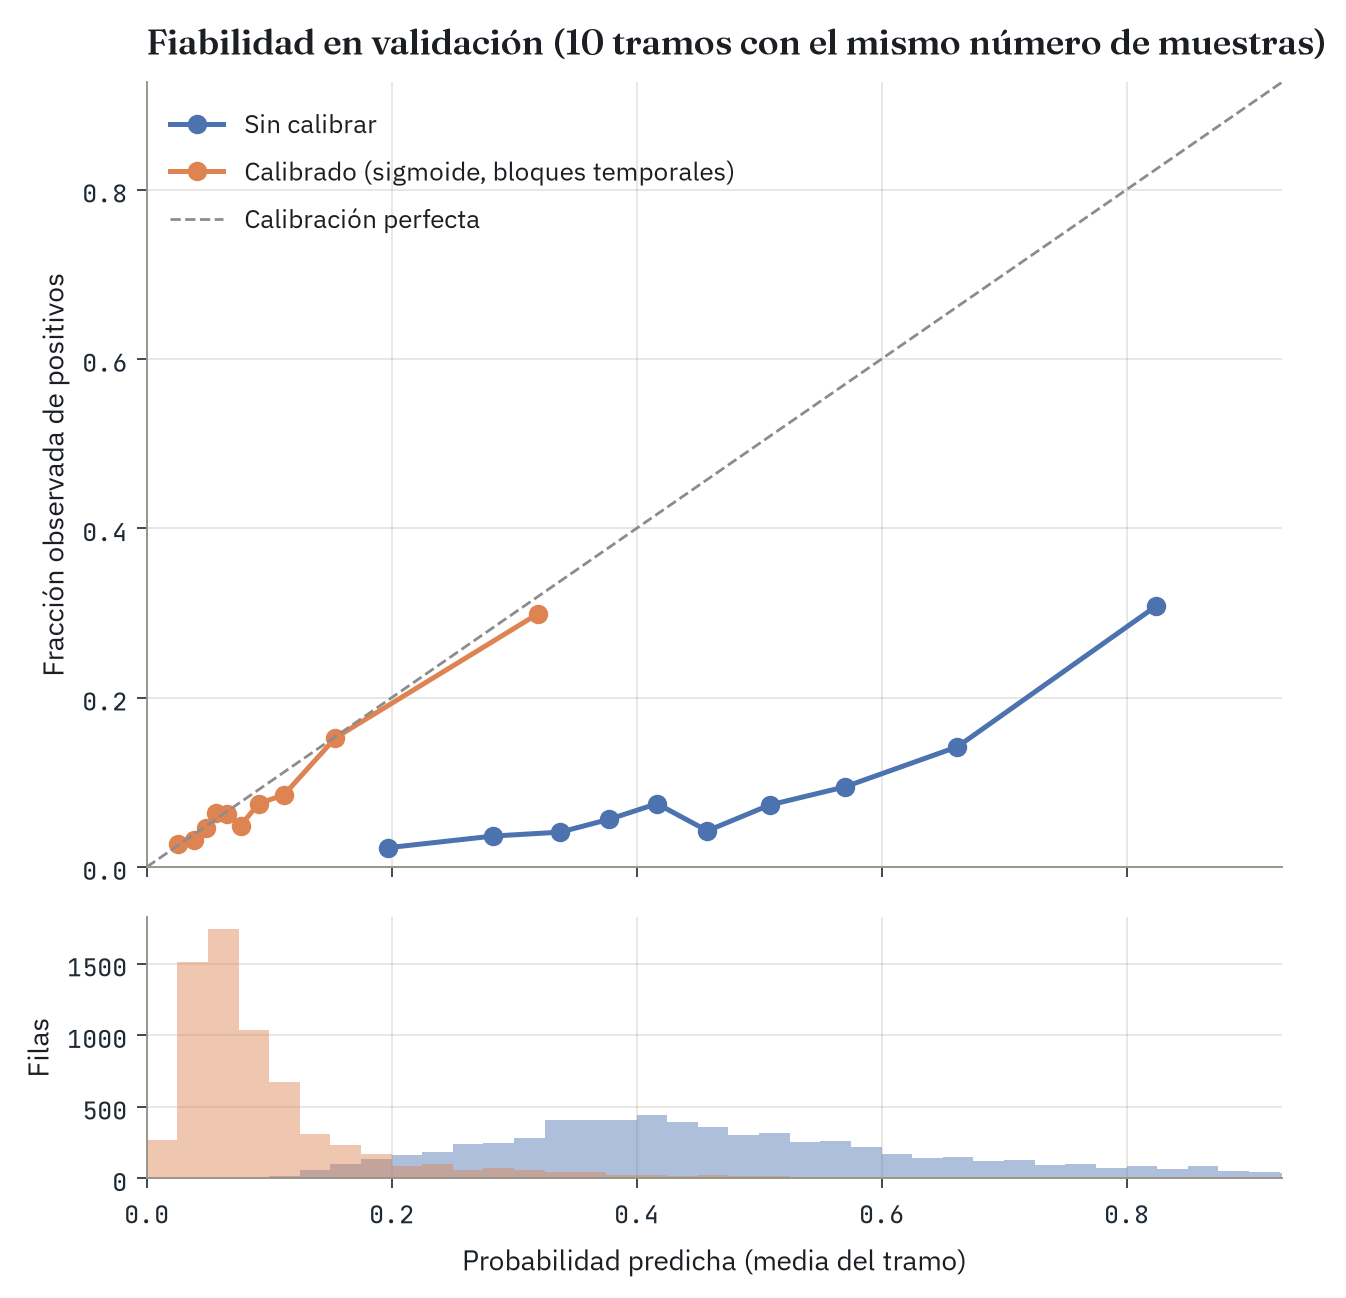
\includegraphics[width=0.46\textwidth]{04_fiabilidad.png}
\caption{Fiabilidad en validación, con tramos del mismo número de muestras:
Sin calibrar (azul) las probabilidades quedan muy por debajo de la diagonal y
muy por encima de la tasa real (\ClfPrevalenciaValidacionPct{}\,\%), mientras
que la calibración sigmoide (naranja) las devuelve a la diagonal y al rango
bajo, donde está casi toda la masa (histograma inferior).}
\label{fig:fiabilidad}
\end{figure}

\subsection{Umbral por costo y alertas por semana}

Con las probabilidades calibradas el umbral de menor costo en validación
coincide con el teórico, $t=\ClfUmbral$ (Figura~\ref{fig:umbrales}), lo que es
una señal de que la calibración funcionó. Con ese umbral se emiten
\ClfAlertasValidacion{} alertas en las \ClfSemanasValidacion{} semanas de
validación, unas \ClfAlertasSemana{} por semana, con $\text{TP}=\ClfTP$,
$\text{FP}=\ClfFP$, $\text{FN}=\ClfFN$ y $\text{TN}=\ClfTN$. Eso da una
precisión de \ClfPrecisionUmbral{}, un recall de \ClfRecallUmbral{} y un F1
de \ClfFUnoUmbral{}. El costo es de \ClfUmbralCosto{} (IC 95\,\% de
\ClfUmbralCostoInf{} a \ClfUmbralCostoSup{}) frente a \ClfCostoNoAlertar{} de
no alertar nunca y \ClfCostoAlertarTodo{} de alertar todas, un ahorro del
\ClfAhorroPct{}\,\% frente a la mejor política sin modelo.

\begin{figure}[!htbp]
\centering
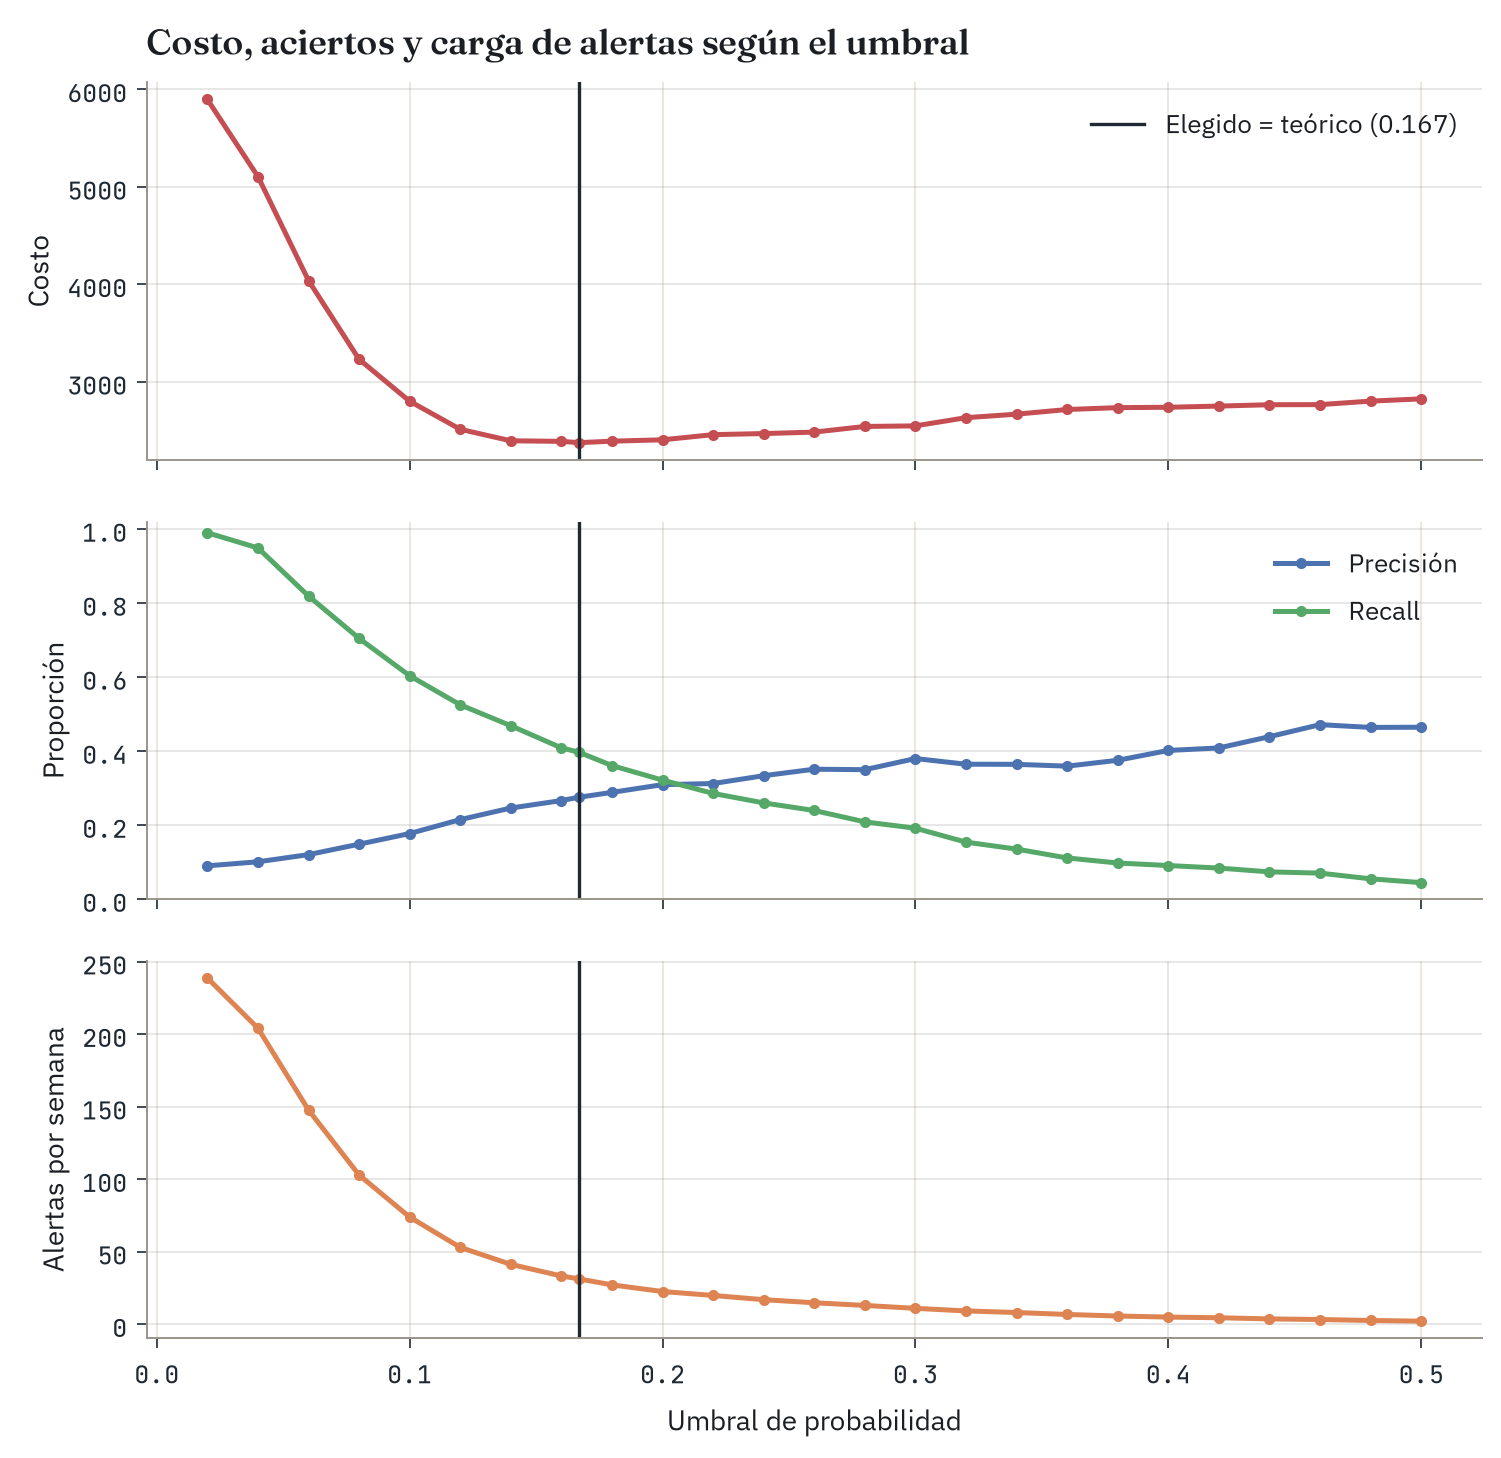
\includegraphics[width=0.48\textwidth]{04_umbrales.png}
\caption{Costo, precisión, recall y alertas por semana según el umbral en
validación, con el umbral elegido como línea vertical: El costo es casi plano
alrededor del umbral teórico mientras que las alertas por semana cambian
mucho a su izquierda.}
\label{fig:umbrales}
\end{figure}

Dicho en términos del laboratorio, por cada no conforme que la alerta detecta
se revisan unas \ClfRevisadasPorDetectado{} muestras que resultan conformes y
aun así se escapa más de la mitad de las no conformes (recall de
\ClfRecallUmbral{}). O sea que la alerta serviría para priorizar la revisión
y no para reemplazar el análisis de todas las muestras. Por último el modelo
congelado (\MakeLowercase{\ClfModeloFinal} calibrada con umbral
\ClfUmbral{}) lo reajustamos con entrenamiento más validación
(\ClfFilasReajuste{} muestras).

% =====================================================================
% redes.tex
% Responsabilidad única: presentar las redes neuronales del curso
% (perceptrón, activaciones, retropropagación, perceptrón multicapa con
% parada temprana) y lo que la red aportó frente a los modelos lineales en
% ambas tareas, con el sobremuestreo y el L16.
% Cifras: macros ClfMLP*, ClfLogisticaParametros, ClfSobre*, ClfModelo*,
% RegRMSE*; figuras 05_red_*; tablas tab:clf-didactica y tab:clf-sobre.
% =====================================================================
\section{Redes neuronales: Del perceptrón al perceptrón multicapa}
\label{sec:redes}

En las dos secciones anteriores el perceptrón multicapa apareció como un
modelo más de la pasada didáctica y como un nivel del factor modelo en los
dos L16, siempre con las mismas variables, los mismos bloques y la misma
métrica que los demás. En las dos tareas perdió frente al modelo lineal y
aquí lo abrimos por dentro (cómo está hecha la red y cómo aprende) para
entender por qué.

\subsection{Del perceptrón a la red con una capa oculta}

Un perceptrón es la unidad más simple de una red. Multiplica cada entrada
por un peso, suma un sesgo y pasa el resultado por una función de activación
$\varphi$, es decir que $\hat{y}=\varphi(\mathbf{w}^\top\mathbf{x}+b)$. Si la
activación es un escalón (como en el perceptrón original) la salida es una
clase y si es la función logística $\sigma(z)=1/(1+e^{-z})$ la salida es una
probabilidad. O sea que la regresión logística de la
Sección~\ref{sec:clasificacion} es en el fondo un perceptrón de una sola
neurona entrenado con la pérdida logarítmica.

El perceptrón multicapa (MLP) mete entre las entradas y la salida una o
varias capas ocultas, cada una con sus propios pesos y una activación no
lineal. La activación es lo que le deja a la red doblar la frontera, porque
sin ella las dos capas se reducirían a una sola suma ponderada, que sería la
misma logística de antes. Con ella la red puede representar interacciones y
umbrales que un modelo lineal no captura. La red que usamos tiene una sola
capa oculta:
\begin{equation}
\mathbf{z}^{(1)}=W_1\mathbf{x}+\mathbf{b}_1,\qquad
\mathbf{h}=\operatorname{ReLU}\!\big(\mathbf{z}^{(1)}\big),\qquad
\hat{p}=\sigma\!\big(\mathbf{w}_2^\top\mathbf{h}+b_2\big),
\label{eq:mlp}
\end{equation}
donde $\hat{p}$ es la probabilidad de que la muestra resulte no conforme.

De las activaciones del curso, la logística va en la salida de un
clasificador binario porque aprieta cualquier valor entre cero y uno y la
tangente hiperbólica es su versión centrada en cero. Las dos se aplanan en los
extremos así que en las capas ocultas encogen el gradiente y la red aprende
muy despacio. La ReLU
($\max(0,z)$) deja pasar la parte positiva y anula la negativa. Como su
derivada es cero o uno no se aplana. Es la que scikit-learn usa por defecto
en las capas ocultas y la que usamos nosotros (\codigo{\ClfMLPActivacion}).

\subsection{Cómo aprende la red: Retropropagación}

La red la entrenamos con \codigo{MLPClassifier}, que en cada lote de $m$ filas
minimiza la pérdida logarítmica (que castiga darle poca probabilidad a lo que
sí pasó) más una penalización $L_2$ sobre el tamaño de los pesos, con
intensidad $\alpha$ (\codigo{alpha}, aquí \ClfMLPAlfa{}) y dividida por el
tamaño del lote:
\begin{equation}
J=-\frac{1}{m}\sum_{i=1}^{m}\Big[y_i\log\hat{p}_i+(1-y_i)\log(1-\hat{p}_i)\Big]
+\frac{\alpha}{2m}\Big(\lVert W_1\rVert^2+\lVert \mathbf{w}_2\rVert^2\Big).
\label{eq:perdida-mlp}
\end{equation}
La retropropagación calcula con la regla de la cadena cuánto cambia $J$ cuando
se mueve cada peso, capa por capa desde la salida hacia la entrada. Con una
salida logística y la pérdida logarítmica la derivada respecto de la entrada
de la neurona de salida se simplifica a $\hat{p}_i-y_i$, que es simplemente
cuánto se equivocó la red con esa muestra. Para los pesos de la capa oculta
todo queda en una sola ecuación,
\begin{equation}
\frac{\partial J}{\partial W_1}
=\frac{1}{m}\Bigg[\sum_{i=1}^{m}
\underbrace{(\hat{p}_i-y_i)}_{\partial J/\partial z^{(2)}}\;
\underbrace{\Big(\mathbf{w}_2\odot\mathbb{1}\big[\mathbf{z}^{(1)}_i>0\big]\Big)}_{\partial z^{(2)}/\partial\mathbf{z}^{(1)}}\;
\underbrace{\mathbf{x}_i^\top}_{\partial\mathbf{z}^{(1)}/\partial W_1}
+\alpha W_1\Bigg],
\label{eq:retropropagacion}
\end{equation}
donde el indicador es la derivada de la ReLU (uno si la neurona estaba
encendida y cero si no) y el término $\alpha W_1$ viene de la penalización,
que empuja los pesos hacia cero. Con ese gradiente el optimizador mueve cada
peso un paso en contra. El que usamos (\codigo{\ClfMLPOptimizador}, el de
scikit-learn por defecto) ajusta el paso de cada peso según cómo se movió su
gradiente en los lotes anteriores.

Una pasada completa por el entrenamiento se llama época. Para que la red no
memorice usamos parada temprana (\codigo{early\_stopping}): La red aparta al
azar el \ClfMLPFraccionValidacionPct{}\,\% de sus filas de ajuste, mide la
exactitud en esa fracción al final de cada época y se detiene cuando lleva
\ClfMLPPaciencia{} épocas sin mejorar, con un tope de \ClfMLPTopeEpocas{}. Así
el número de épocas funciona como una segunda regularización. Eso sí, esa
fracción se aparta al azar y no por fecha así que la parada vigila el error
dentro del mismo periodo. La comparación entre modelos, en cambio, sigue
usando los bloques temporales.

\subsection{La red que usamos y su entrenamiento}

La red tiene \ClfMLPEntradas{} entradas (las columnas que deja el
preprocesamiento del grupo ampliado), una capa oculta de \ClfMLPOcultas{}
neuronas ReLU y una salida logística (Figura~\ref{fig:red-arquitectura}). En
total son \ClfMLPParametros{} pesos y sesgos frente a los
\ClfLogisticaParametros{} coeficientes de la regresión logística con las
mismas entradas, o sea unas \ClfMLPVecesParametros{} veces más.

\begin{figure}[!htbp]
\centering
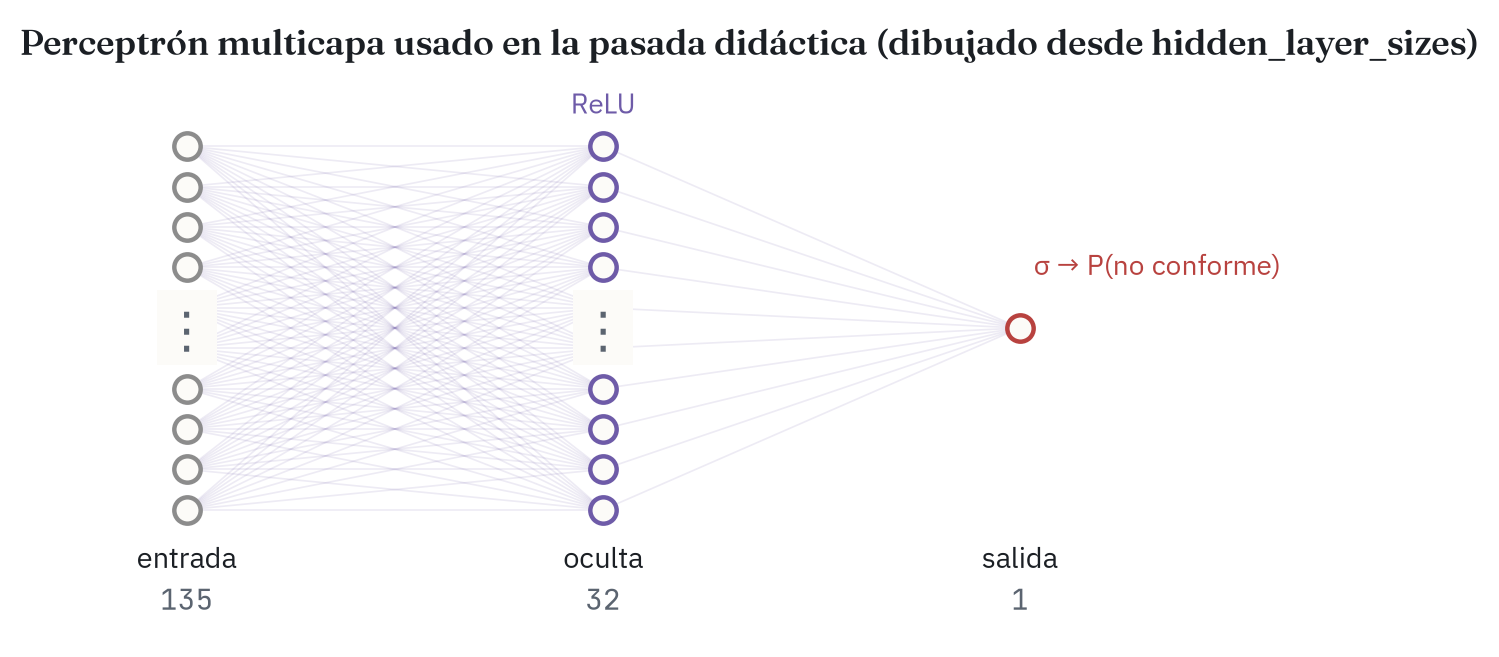
\includegraphics[width=0.52\textwidth]{04_red_arquitectura.png}
\caption{Arquitectura del perceptrón multicapa de la pasada didáctica,
dibujada desde \codigo{hidden\_layer\_sizes}: Las capas grandes se muestran
recortadas y casi todos los parámetros están en las conexiones entre la
entrada y la capa oculta.}
\label{fig:red-arquitectura}
\end{figure}

Cuando la ajustamos una vez con todo el entrenamiento la red se detuvo en la
época \ClfMLPEpocas{}, \ClfMLPPaciencia{} después de la mejor
(\ClfMLPMejorEpoca{}), como se ve en la Figura~\ref{fig:red-curvas}. La pérdida
de entrenamiento siguió bajando hasta \ClfMLPPerdidaFinal{}, mientras que la
exactitud en la fracción apartada llegó como máximo a
\ClfMLPExactitudMejor{}, apenas por encima de la que se obtiene diciendo
siempre ``conforme'' (\ClfTasaMayoritaria{}). Esto explica parte del
problema: Con tan pocas no conformes la exactitud casi no distingue un modelo
que ordena bien de uno que no así que la parada temprana de scikit-learn
está vigilando una señal muy débil. Por eso en todo el proyecto comparamos
los modelos con el ROC-AUC y no con la exactitud.

\begin{figure}[!htbp]
\centering
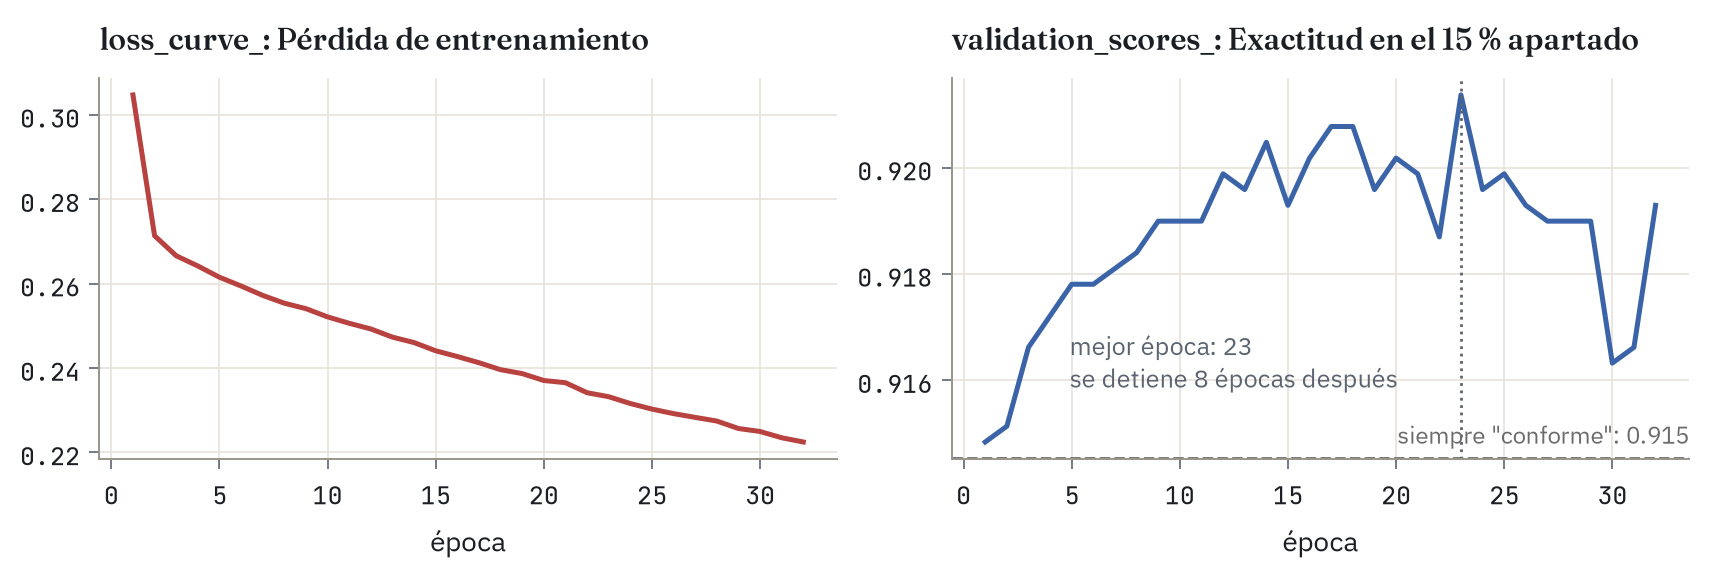
\includegraphics[width=0.84\textwidth]{04_red_curvas.png}
\caption{Curvas de la red ajustada con todo el entrenamiento, con la pérdida
logarítmica por época (\codigo{loss\_curve\_}) y la exactitud en la fracción
apartada (\codigo{validation\_scores\_}): La pérdida sigue bajando mientras
la exactitud se queda pegada a la de responder siempre ``conforme''
(discontinua) y la punteada marca la mejor época.}
\label{fig:red-curvas}
\end{figure}

\subsection{Qué aportó la red frente a los modelos lineales}

La respuesta corta es que en estos datos no le ganó al modelo lineal. En clasificación la red obtuvo
en la pasada didáctica un ROC-AUC medio de \ClfAUCMLPDidactico{} frente a
\ClfAUCLogisticaDidactico{} de la regresión logística
(Tabla~\ref{tab:clf-didactica}) y en regresión un RMSE medio de
\RegRMSEMLPDidactico{} frente a \RegRMSELinealDidactico{} de la regresión
lineal múltiple (Tabla~\ref{tab:reg-didactica}). Le dimos varias vueltas a si
una red más grande o con menos penalización ordenaría mejor y en la regresión
la rejilla tampoco cambió el orden (\RegRejillaMLPRMSE{} frente a
\RegRejillaLinealRMSE{}). O sea que pese a tener muchos más parámetros la red
no mejora al modelo lineal en ninguna de las dos tareas. Nuestra lectura es
que en estos datos simulados la señal está sobre todo en efectos que se suman
(en la escala de la carga o en la del logit) y que el modelo lineal ya los
captura así que la capa oculta no encuentra interacciones que compensen lo que
cuesta en varianza y en interpretación ya que la red no da razones de odds
que se puedan leer.

El sobremuestreo agrava la diferencia. Es al
\MakeLowercase{\ClfSobreMasPierde} al que más ROC-AUC le quita
(\ClfSobreDeltaAUC{}, Tabla~\ref{tab:clf-sobre}), mientras que a la
\MakeLowercase{\ClfSobreMenosPierde} casi no la cambia
(\ClfSobreDeltaAUCMenor{}). Una explicación posible, que no comprobamos por
separado, es que el sobremuestreo aleatorio repite filas no conformes que una
red con \ClfMLPParametros{} parámetros puede memorizar. Además las copias de
una misma fila pueden caer a la vez en la parte de ajuste y en la fracción
que vigila la parada temprana, de modo que la parada deja de notar el
sobreajuste. La logística, con \ClfLogisticaParametros{} coeficientes, casi
no tiene cómo memorizar.

El L16 de clasificación cuenta lo mismo desde otro diseño: En el
factor \ClfFactorPrincipal{} el mejor nivel es la \ClfModeloMejorNivel{} (S/N
media de \ClfSNModeloMejor{} dB) y el peor el \ClfModeloPeorNivel{}
(\ClfSNModeloPeor{} dB). Como cada nivel se promedia sobre corridas con y sin
sobremuestreo, parte de esa diferencia viene de lo que el sobremuestreo le
hace a la red. Con datos reales podría haber interacciones
que el generador no tiene así que antes de descartar la red repetiríamos la
comparación.

% =====================================================================
% bayes.tex
% Responsabilidad única: presentar la probabilidad de falso positivo
% (teoría, sensibilidad y especificidad por controles, VPP por ensayo y por
% muestra, posterior tras el reensayo, regla de reensayo y auditoría de la
% simulación). Cifras: macros Clf* de Bayes; tablas tabla_bayes_*.
% =====================================================================
\section{Probabilidad de falso positivo}
\label{sec:bayes}

La tercera pregunta no la respondemos con un modelo entrenado sino con el
teorema de Bayes. Para eso juntamos lo que dicen los controles de calidad del
laboratorio con la probabilidad calibrada del clasificador anterior.

\subsection{Planteamiento}

Un resultado no conforme puede salir porque el producto está contaminado o
porque el ensayo falló (una contaminación dentro del laboratorio o un error
de lectura) y lo que el laboratorio quiere saber es qué tan probable es lo
segundo. Para eso hacen falta tres cosas. La sensibilidad $S$ es la
probabilidad de que el ensayo dé positivo cuando sí hay contaminación, la
especificidad $E$ es la probabilidad de que dé negativo cuando no la hay y
$\pi$ es la prevalencia real de contaminación. Con ellas el teorema de Bayes
da el valor predictivo positivo (VPP, la probabilidad de que un positivo sea
de verdad) y su complemento, que es la probabilidad de falso positivo:
\[
\mathrm{VPP}=\frac{S\,\pi}{S\,\pi+(1-E)(1-\pi)},\qquad
P(\text{falso positivo}\mid +)=1-\mathrm{VPP}.
\]
La prevalencia real no se observa porque lo que vemos es la proporción $p$
de positivos, que mezcla verdaderos y falsos. De esa proporción se despeja
$\pi$ con la corrección de Rogan y Gladen \cite{rogan1978},
$\pi=\bigl(p-(1-E)\bigr)/(S+E-1)$, recortada para que quede entre cero y uno.

\subsection{Sensibilidad y especificidad desde los controles}

El laboratorio siembra a diario controles positivos (que llevan el
microorganismo) y negativos (estériles). La sensibilidad es entonces la
fracción de controles positivos que crecen y la especificidad la fracción de
negativos que no crecen. Con los \ClfControlesDesarrollo{} controles del
desarrollo las estimamos para los \ClfEnsayos{} ensayos (columnas Sens.\ y
Espec.\ de la Tabla~\ref{tab:vpp-ensayo}, con sus intervalos de Wilson de
95\,\% en el notebook). La sensibilidad va de \ClfSensMin{}
(\textit{\ClfSensMinEnsayo}) a \ClfSensMax{} y la especificidad de
\ClfEspecMin{} (\ClfEspecMinEnsayo) a \ClfEspecMax{}.

\subsection{VPP por ensayo y por muestra}

Con la proporción de positivos de cada ensayo en el desarrollo y sus $S$ y $E$
calculamos el VPP por ensayo (Tabla~\ref{tab:vpp-ensayo}), que va de
\ClfVPPPeor{} en \ClfVPPPeorEnsayo{} (intervalo de \ClfVPPPeorInf{} a
\ClfVPPPeorSup{}) a \ClfVPPMejor{} en \textit{\ClfVPPMejorEnsayo}. Los
intervalos salen de \ClfSorteos{} sorteos de las distribuciones Beta de $p$,
$S$ y $E$ (que describen lo que no sabemos de cada una) y la fracción de
positivos cuya previa hubo que recortar a cero fue de
\ClfRecorteCeroPct{}\,\%. Ponderado por positivos el VPP del laboratorio es
de \ClfVPPGlobal{}, o sea que según los controles unos \ClfFalsosPorCien{} de
cada cien resultados no conformes serían falsos.

\begin{table}[!htbp]
\centering
\tablaancha{bayes_vpp_ensayo}
\caption{VPP por ensayo en el desarrollo, con la prevalencia corregida por
Rogan y Gladen: Los ensayos con pocos positivos (\textit{Salmonella} y
esterilidad) son los de intervalos más anchos.}
\label{tab:vpp-ensayo}
\end{table}

El VPP por ensayo trata igual a todas las muestras de un mismo ensayo, cuando
en realidad la probabilidad previa de contaminación cambia de una muestra a
otra. Por eso lo combinamos con el clasificador de la
Sección~\ref{sec:clasificacion}. Su probabilidad calibrada $p(x)$ de resultar
no conforme la corregimos con Rogan y Gladen para obtener una previa propia de
cada muestra, $\pi(x)$, que entra a la fórmula del VPP en lugar de $\pi$. Aquí
se ve por qué nos importaba tanto la calibración ya que si $p(x)$ no fuera
una probabilidad esta previa no tendría sentido. Entre los
\ClfPositivosValidacionBayes{} positivos de validación el VPP$(x)$ va de
\ClfVPPxMin{} a \ClfVPPxMax{}, con percentiles 10 y 90 de \ClfVPPxPDiez{} y
\ClfVPPxPNoventa{}. Por ejemplo en \ClfEnsayoEjemplo{} la probabilidad de que
el positivo sea falso es de \ClfFalsoRiesgoBajo{} en una muestra de riesgo
bajo y de \ClfFalsoRiesgoAlto{} en una de riesgo alto. Es decir que el mismo
resultado merece más o menos desconfianza según la muestra de la que viene.

\subsection{Reensayo y regla de reensayo}

Si un positivo se reensaya, la probabilidad se actualiza con el segundo
resultado. Después de dos positivos queda entre \ClfPosteriorMasMasMin{} y
\ClfPosteriorMasMasMax{} según el ensayo, mientras que después de un positivo
y un negativo cae a un rango de \ClfPosteriorMasMenosMin{} a
\ClfPosteriorMasMenosMax{}. O sea que un reensayo conforme vuelve probable el
falso positivo pero no lo asegura. Los controles anticipan que el
\ClfReensayoConformeEsperadoPct{}\,\% de los reensayos salga conforme y en los
\ClfReensayados{} positivos reensayados del desarrollo observamos el
\ClfReensayoConformeObservadoPct{}\,\%, una cifra cercana.

El cribado había mostrado que el análisis
\codigo{falso\_positivo\_lectura} no necesita un modelo porque una sola
variable basta. Esa variable es la razón entre el recuento y el límite de
la norma. La Figura~\ref{fig:regla} lo muestra por sextiles (seis grupos con
el mismo número de reensayos). Cuando $\log_{10}(\text{recuento}/\text{límite})$
es menor que \ClfReglaBorde{}, es decir cuando el recuento supera el límite en
menos de \ClfReglaVecesLimite{} veces, el \ClfReglaTasaBajoPct{}\,\% de los
reensayos sale conforme frente al \ClfReglaTasaAltoPct{}\,\% por encima del
borde. Ese grupo es apenas el \ClfReglaGrupoPct{}\,\% de los reensayados con
recuento pero concentra el \ClfReglaCapturaPct{}\,\% de los reensayos
conformes. La regla que proponemos es entonces sencilla: Reensayar sobre todo
los no conformes cuyo recuento quede por debajo de \ClfReglaVecesLimite{}
veces el límite. En los ensayos sin recuento (los de presencia o ausencia) la
regla no aplica y allí, de \ClfSinRazonReensayados{} reensayados, una fracción
de \ClfSinRazonConformes{} resultó conforme.

\subsection{Auditoría frente a la verdad de la simulación}
\label{sec:auditoria-bayes}

\textbf{Esta subsección solo es posible con datos simulados} porque usa la
``verdad oculta'' del generador (qué muestras estaban de verdad
contaminadas), que con datos reales no existe. Sirve para comprobar que el
método recupera lo que el generador puso y no para describir el laboratorio.
El VPP real del desarrollo es de \ClfAudVPPReal{} frente a \ClfVPPGlobal{}
estimado y el VPP real de \ClfAudEnsayosDentroIC{} de los \ClfEnsayos{}
ensayos cae dentro del intervalo estimado (Figura~\ref{fig:auditoria}). La
especificidad de los controles supera en promedio a la que de verdad tienen
las muestras en \ClfAudSesgoEspec{} porque en las muestras hay fuentes de
error que los controles no sufren. Parece poco, pero en los ensayos de menor
prevalencia basta para que el VPP estimado quede por encima del real. Entre
los reensayados la fracción realmente no contaminada es de
\ClfAudFalsoRealReensayados{}. Por último el VPP$(x)$ ordena mejor la
contaminación real que el VPP por ensayo (ROC-AUC de \ClfAudAUCVPPx{} frente
a \ClfAudAUCVPPEnsayo{} y Brier de \ClfAudBrierVPPx{} frente a
\ClfAudBrierVPPEnsayo{}), lo que respalda usar la previa por muestra.

\begin{figure}[!htbp]
\centering
\begin{minipage}[t]{0.49\textwidth}\centering
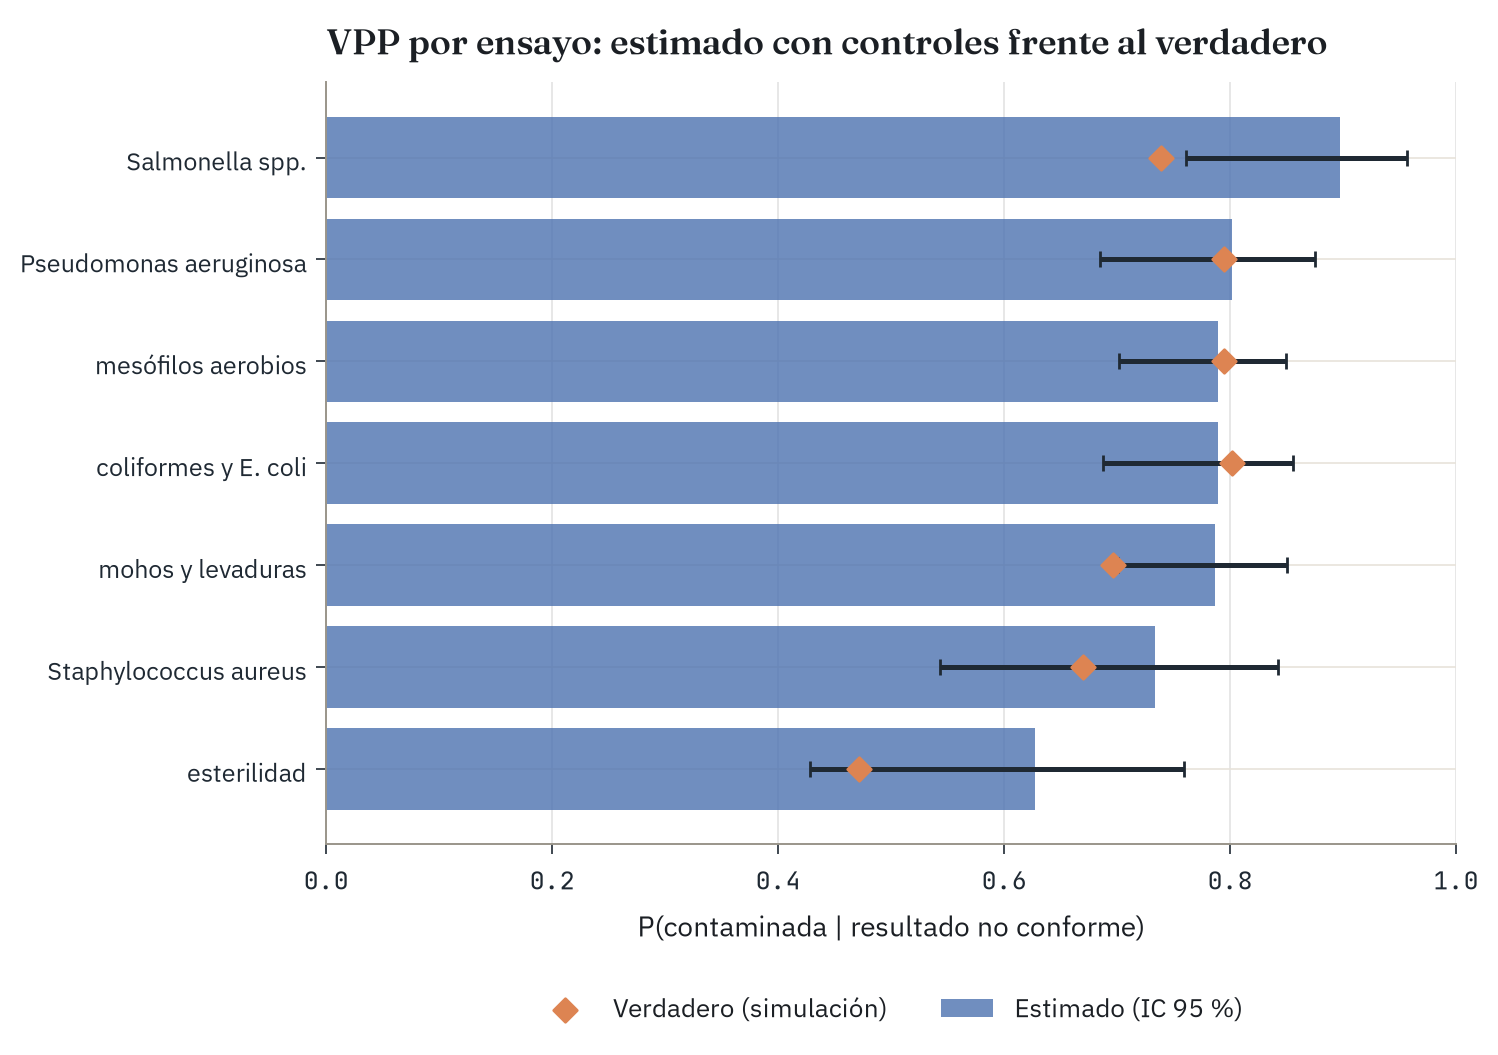
\includegraphics[width=\textwidth]{04_auditoria_vpp.png}
\caption{\textbf{Auditoría con la verdad de la simulación.} VPP por ensayo
estimado con los controles (barras con IC 95\,\%) frente al verdadero
(rombos): Los rombos que caen fuera del intervalo (\textit{Salmonella} y
mohos y levaduras) son los ensayos donde la estimación es optimista.}
\label{fig:auditoria}
\end{minipage}\hfill
\begin{minipage}[t]{0.49\textwidth}\centering
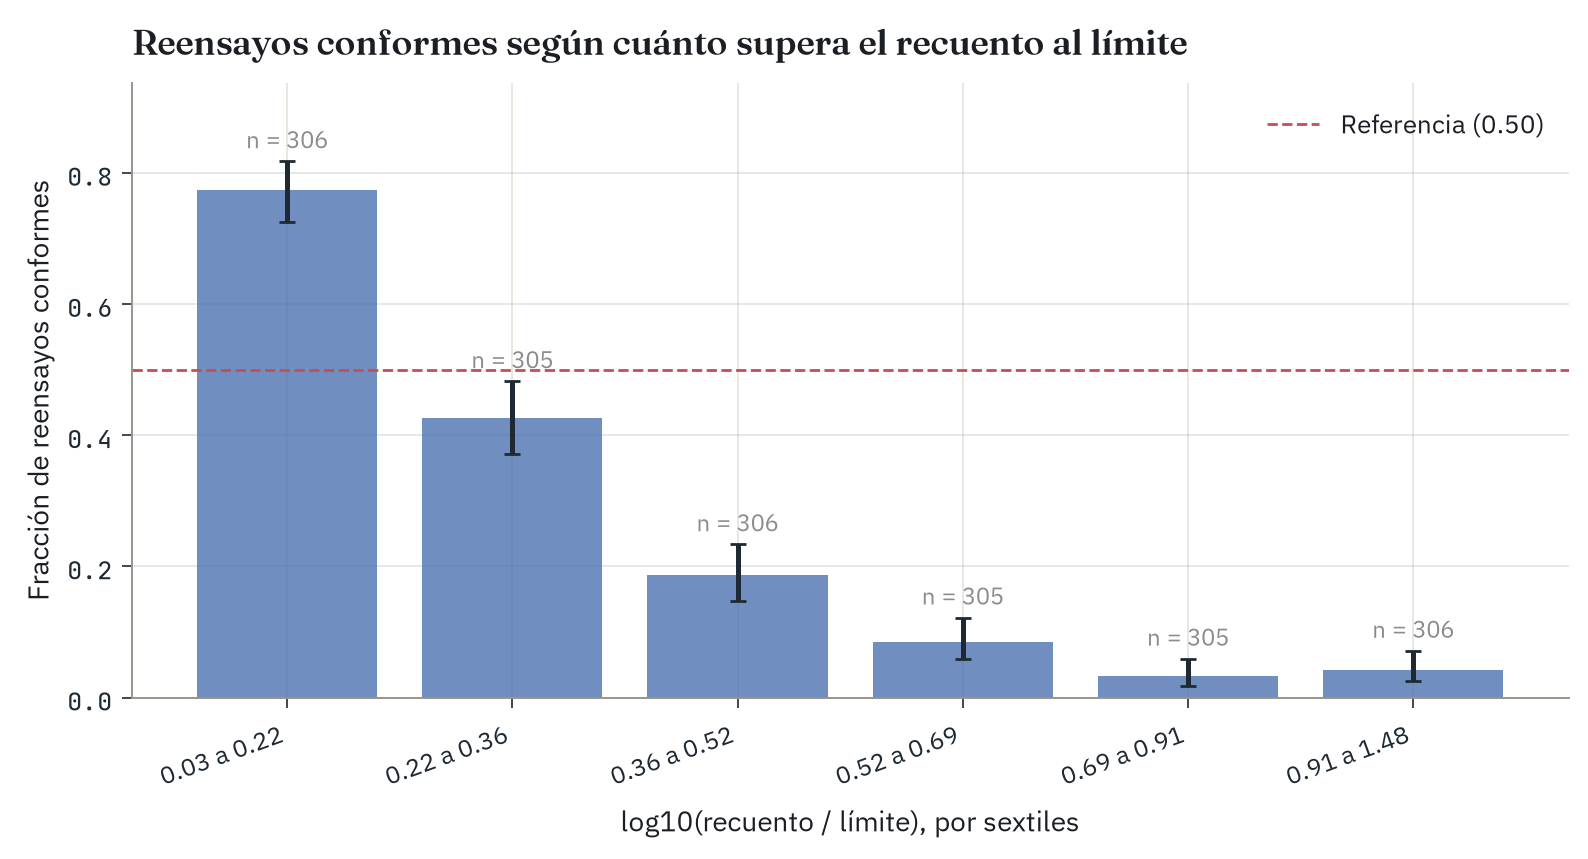
\includegraphics[width=\textwidth]{04_regla_reensayo.png}
\caption{Fracción de reensayos conformes según cuánto supera el recuento al
límite, por sextiles y con IC de Wilson: La caída es abrupta después del
primer sextil, que es el que define el borde de la regla de reensayo.}
\label{fig:regla}
\end{minipage}
\end{figure}

% =====================================================================
% agrupamiento.tex
% Responsabilidad única: presentar los perfiles de muestra (análisis
% elegido) y los segmentos de clientes (complementario), la diferencia de
% silueta entre el cribado y la etapa 06 y por qué se mantuvo la selección.
% Cifras: macros Agr*; tablas tabla_agr_*; figuras 06_*.
% =====================================================================
\section{Agrupamiento: perfiles de muestra y segmentos de clientes}
\label{sec:agrupamiento}

El agrupamiento no tiene una respuesta correcta contra la cual medirse, así
que se usa de forma descriptiva y con dos controles de honestidad, el
estadístico de Hopkins (tendencia a agruparse, 0.5 para datos sin estructura)
y la estabilidad de los grupos al cambiar la semilla. Se estudian dos
análisis, el elegido por la regla, \codigo{\AgrSeleccionado}
(\AgrSelFilas{} muestras aceptadas, \AgrSelVariables{} variables, de las
cuales \AgrSelConLog{} con $\log(1+x)$), y el complementario,
\codigo{\AgrComplementario} (\AgrCompFilas{} clientes, \AgrCompVariables{}
variables agregadas).

\paragraph{Escalado.} Sin escalar, la variable \AgrSelDominante{} aporta el
\AgrSelDominantePct{}\,\% de la varianza de los perfiles de muestra (y la
\AgrCompDominante{} el \AgrCompDominantePct{}\,\% en los segmentos), de forma
que K-means agruparía por una sola variable; el acuerdo (ARI) entre la
solución sin escalar y la escalada es de \AgrSelARISinEscalar{}, así que el
escalado no es un detalle, cambia por completo los grupos.

\subsection{Perfiles de muestra}

Con la matriz escalada (Hopkins de \AgrSelHopkins{}) se exploró K-means con
$k$ de \AgrKMin{} a \AgrKMax{}, con siluetas entre \AgrSelSiluetaMin{} y
\AgrSelSiluetaMax{}, y se eligió $k=\AgrSelK$ (silueta de
\AgrSelSilueta{}). La silueta es baja, es decir, las fronteras entre grupos
son difusas, pero la solución es estable, con un ARI entre
\AgrSelEstabilidadMin{} y \AgrSelEstabilidadMax{} frente a
\AgrSemillasEstabilidad{} semillas adicionales. La
Tabla~\ref{tab:agr-perfiles} nombra cada grupo por las variables que se
apartan más de \AgrUmbralNombre{} desviaciones estándar de la media.

\begin{table}[!htbp]
\centering
\tablaancha{agr_sel_grupos}
\caption{Perfiles de muestra de K-means, nombrados por las variables que los
distinguen (en desviaciones estándar, DE, respecto a la media general).}
\label{tab:agr-perfiles}
\end{table}

DBSCAN, con $\varepsilon=\AgrSelDBEps$ y \codigo{min\_samples} de
\AgrSelDBMinMuestras{} (\AgrSelDBConGrupos{} de las
\AgrSelDBCombinaciones{} combinaciones de la rejilla dieron dos o más grupos),
encuentra \AgrSelDBGrupos{} grupos densos con un \AgrSelDBRuidoPct{}\,\% de
ruido y una silueta sin ruido de \AgrSelDBSilueta{}, y su acuerdo con K-means
es bajo (ARI de \AgrSelARIKmDb{}). La Figura~\ref{fig:agr-pca} muestra por
qué, ya que K-means parte una nube continua en regiones, mientras que DBSCAN
solo separa la zona densa aislada, que coincide con el perfil de plazo
prometido largo.

\begin{figure}[!htbp]
\centering
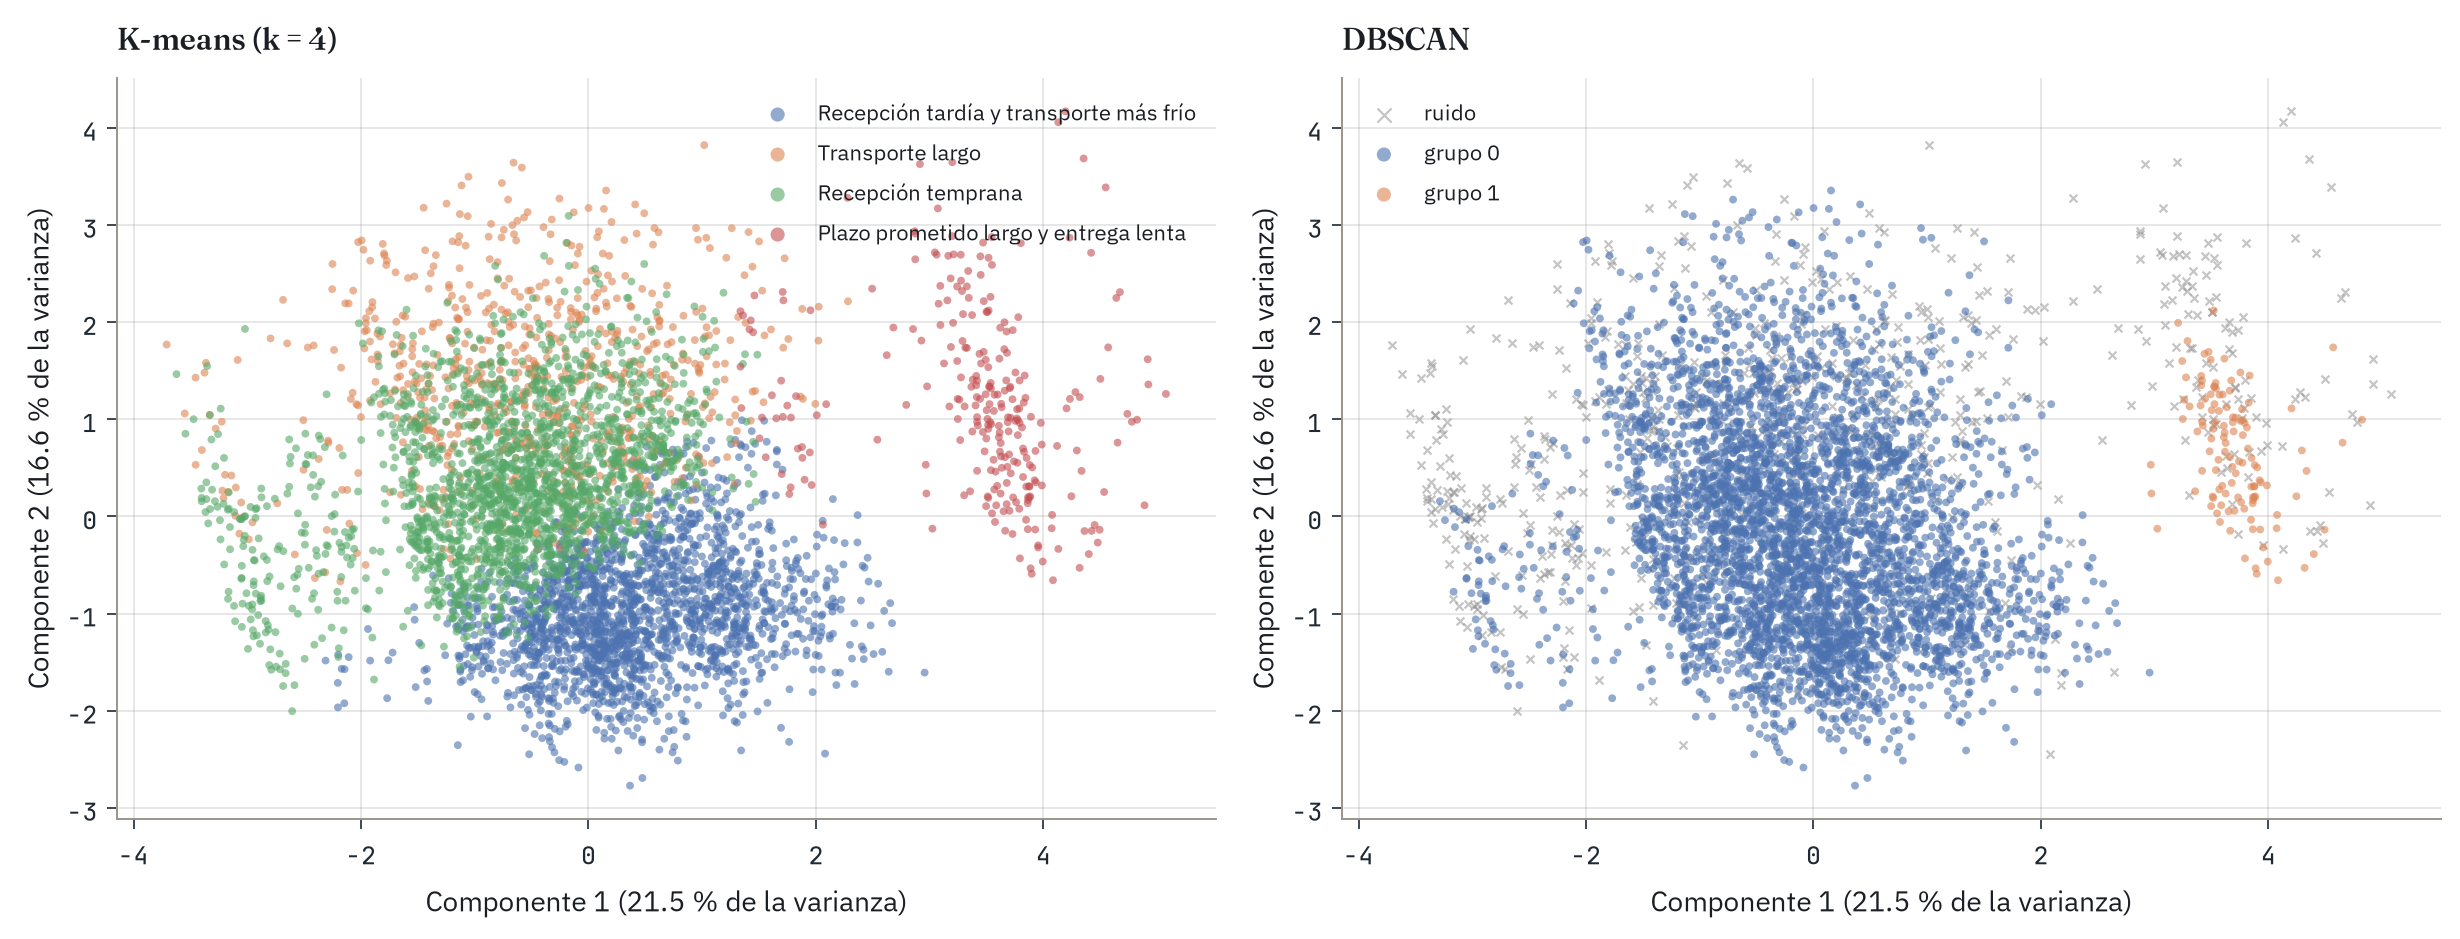
\includegraphics[width=0.85\textwidth]{06_perfiles_muestra_pca.png}
\caption{Perfiles de muestra en las dos primeras componentes principales
(\AgrSelPCAVarianzaPct{}\,\% de la varianza): K-means (izquierda) y DBSCAN
(derecha, ruido en gris). La única región bien separada es la de la derecha;
el resto es una nube continua que K-means corta en franjas.}
\label{fig:agr-pca}
\end{figure}

\subsection{Segmentos de clientes}

En los clientes (Hopkins de \AgrCompHopkins{}) se eligió $k=\AgrCompK$, con
una silueta de \AgrCompSilueta{} y una estabilidad entre
\AgrCompEstabilidadMin{} y \AgrCompEstabilidadMax{}. El segmento más grande
en volumen, «\AgrCompSegmentoMayor», reúne el
\AgrCompSegmentoMayorClientesPct{}\,\% de los clientes pero el
\AgrCompSegmentoMayorMuestrasPct{}\,\% de las muestras, y el segmento de más
no conformidad es también el de más entregas tardías
(Figura~\ref{fig:agr-segmentos}), lo que lo
hace el candidato natural para un seguimiento comercial y de calidad. En este
análisis DBSCAN no encontró dos grupos con ninguna combinación
(\AgrCompDBConGrupos{} de \AgrCompDBCombinaciones{}), así que se usa como
detector de atípicos ($\varepsilon=\AgrCompDBEps$, \AgrCompDBRuidoPct{}\,\% de
clientes marcados como ruido).

\begin{figure}[!htbp]
\centering
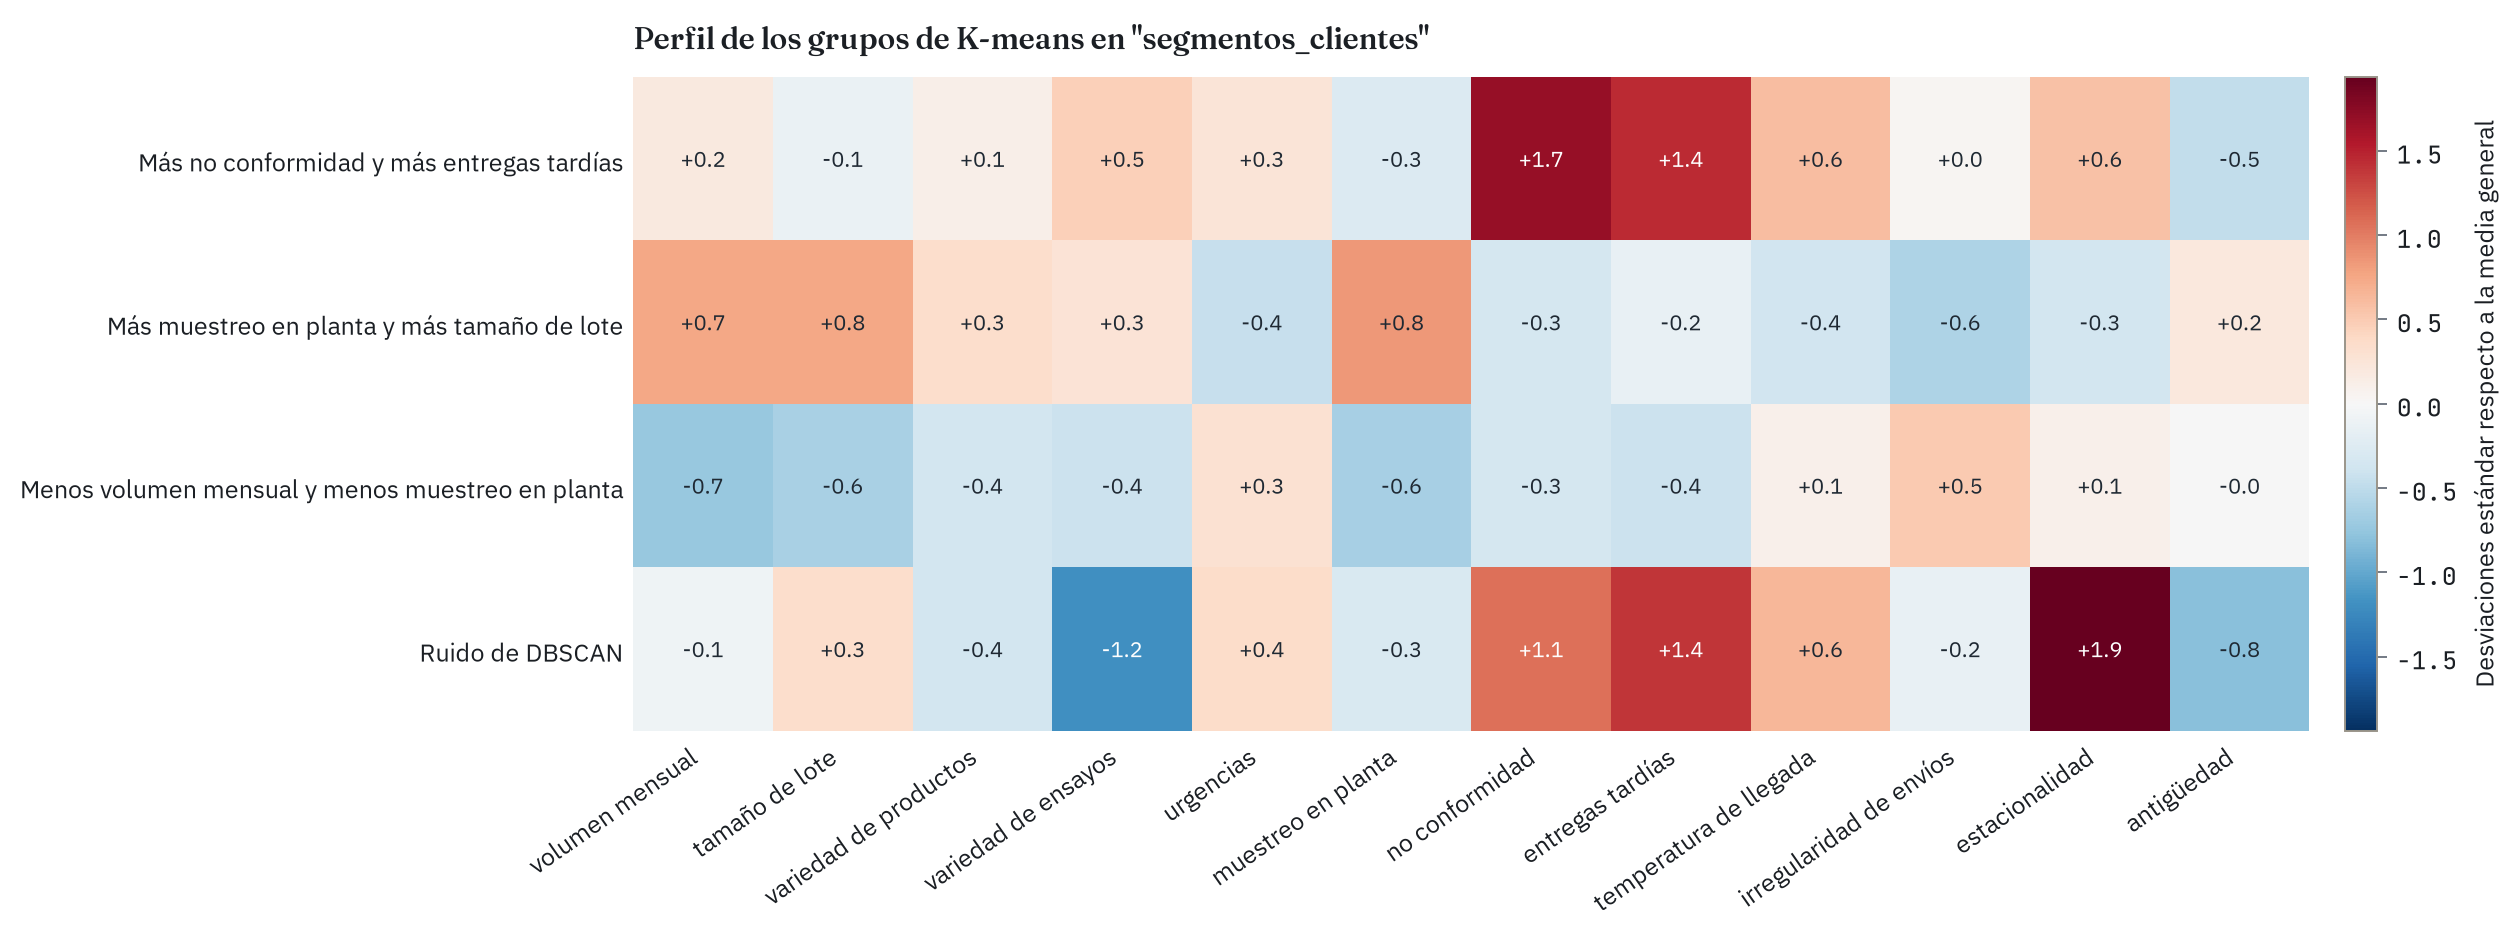
\includegraphics[width=0.9\textwidth]{06_segmentos_clientes_perfiles.png}
\caption{Perfil de los segmentos de clientes (desviaciones estándar respecto a
la media general). La fila inferior son los clientes que DBSCAN marca como
ruido: comparten la no conformidad y las entregas tardías altas del primer
segmento, pero con una estacionalidad mucho más marcada.}
\label{fig:agr-segmentos}
\end{figure}

\subsection{Silueta del cribado frente a la etapa 06}
\label{sec:silueta}

La silueta de los perfiles de muestra cae de \AgrSiluetaCribado{} en el
cribado a \AgrSelSilueta{} en la etapa~06, muy por encima de la diferencia
de \AgrToleranciaSilueta{} a partir de la cual el procedimiento la discute, y la
etapa~06 separa sus dos causas (Tabla~\ref{tab:agr-silueta}). El cambio de
filas (entrenamiento frente a todo el desarrollo) mueve la silueta en
\AgrEfectoFilas{} (\AgrSiluetaSinLog{} sin $\log(1+x)$), mientras que la
transformación $\log(1+x)$ antes de escalar la mueve en \AgrEfectoLog{}, de
forma que casi toda la caída se debe al preprocesamiento; una explicación
plausible (no verificada por separado) es que, sin el logaritmo, las colas
largas de unas pocas variables separan dos grupos con facilidad, y con él esa
separación desaparece.

\begin{table}[!htbp]
\centering
\tablaancha{agr_silueta_cribado}
\caption{Silueta y puntaje de la regla con el preprocesamiento del cribado y
con el de la etapa 06, para los dos análisis de agrupamiento.}
\label{tab:agr-silueta}
\end{table}

Con las siluetas de la etapa~06, el puntaje de la regla sería de
\AgrPuntajeSelEtapa{} para el análisis elegido y de \AgrPuntajeCompEtapa{}
para el complementario, es decir, el complementario habría ganado
(\AgrComplementarioSupera{}). Aun así se mantuvo la selección, porque la regla
se fijó antes de ver los resultados y cambiarla después equivaldría a elegir
a posteriori; en su lugar se reportan los dos análisis completos y
la discrepancia queda registrada como una lección para el cribado, que debe
usar el mismo preprocesamiento que el estudio a fondo.

\paragraph{Auditoría con la verdad de la simulación.} Solo con datos
simulados se puede comparar con los \AgrAudSegmentosLatentes{} segmentos
latentes del generador: en los \AgrAudClientes{} clientes auditados, el ARI
es de \AgrAudARIKmeans{} para K-means y de \AgrAudARIDbscan{} para DBSCAN, con
una pureza de \AgrAudPureza{}. Los segmentos recuperan solo en parte la
estructura latente, lo que es coherente con que el generador hace que los
segmentos se solapen a propósito.

% =====================================================================
% evaluacion.tex
% Responsabilidad única: presentar la evaluación única en prueba de los
% modelos congelados, lado a lado con validación (regresión, clasificación
% y Bayes), con el umbral retrospectivo marcado como no usado.
% Cifras: macros Fin*; tablas tabla_final_*; figuras 07_*.
% =====================================================================
\section{Evaluación final en prueba}
\label{sec:evaluacion}

Antes de abrir la prueba (\FinPruebaDesde{} a \FinPruebaHasta{}) quedaron
registrados los modelos congelados (Tabla~\ref{tab:congelado}), y la prueba
se leyó una sola vez, en la etapa~07; nada de lo que sigue se usó para cambiar
un modelo, una variable o un umbral.

\begin{table}[!htbp]
\centering
\tablaancha{final_congelado}
\caption{Modelos congelados antes de abrir la prueba, con la cifra de
validación que justificó cada uno.}
\label{tab:congelado}
\end{table}

\subsection{Regresión}

En los \FinDiasPrueba{} días hábiles de prueba, la regresión lineal obtuvo un
RMSE de \FinRMSEPrueba{} (IC 95\,\% de \FinRMSEPruebaInf{} a
\FinRMSEPruebaSup{}), un MAE de \FinMAEPrueba{}, un $R^2$ de
\FinRDosPrueba{} y una habilidad de \FinHabilidadPrueba{} (de
\FinHabilidadPruebaInf{} a \FinHabilidadPruebaSup{}) frente a
\codigo{\FinRegReferencia} (Tabla~\ref{tab:final-reg}). El RMSE cambió un
\FinCambioRMSEPct{}\,\% respecto a validación, es decir, el modelo se
equivocó menos en prueba, pero eso no prueba que haya mejorado: la carga media
de prueba (\FinMediaPrueba{} muestras por día hábil) es menor que la de
validación (\RegMediaValidacion{}), y con un nivel más bajo los errores
absolutos también tienden a serlo. La habilidad, que se mide frente a la
referencia del mismo periodo, también subió, y su intervalo se solapa con el
de validación, así que lo prudente es leer ambos periodos como compatibles.

\begin{table}[!htbp]
\centering
\small
\tablagen{final_regresion_validacion}
\caption{Regresión: validación frente a prueba, con intervalo bootstrap de
95\,\% en prueba.}
\label{tab:final-reg}
\end{table}

\begin{figure}[!htbp]
\centering
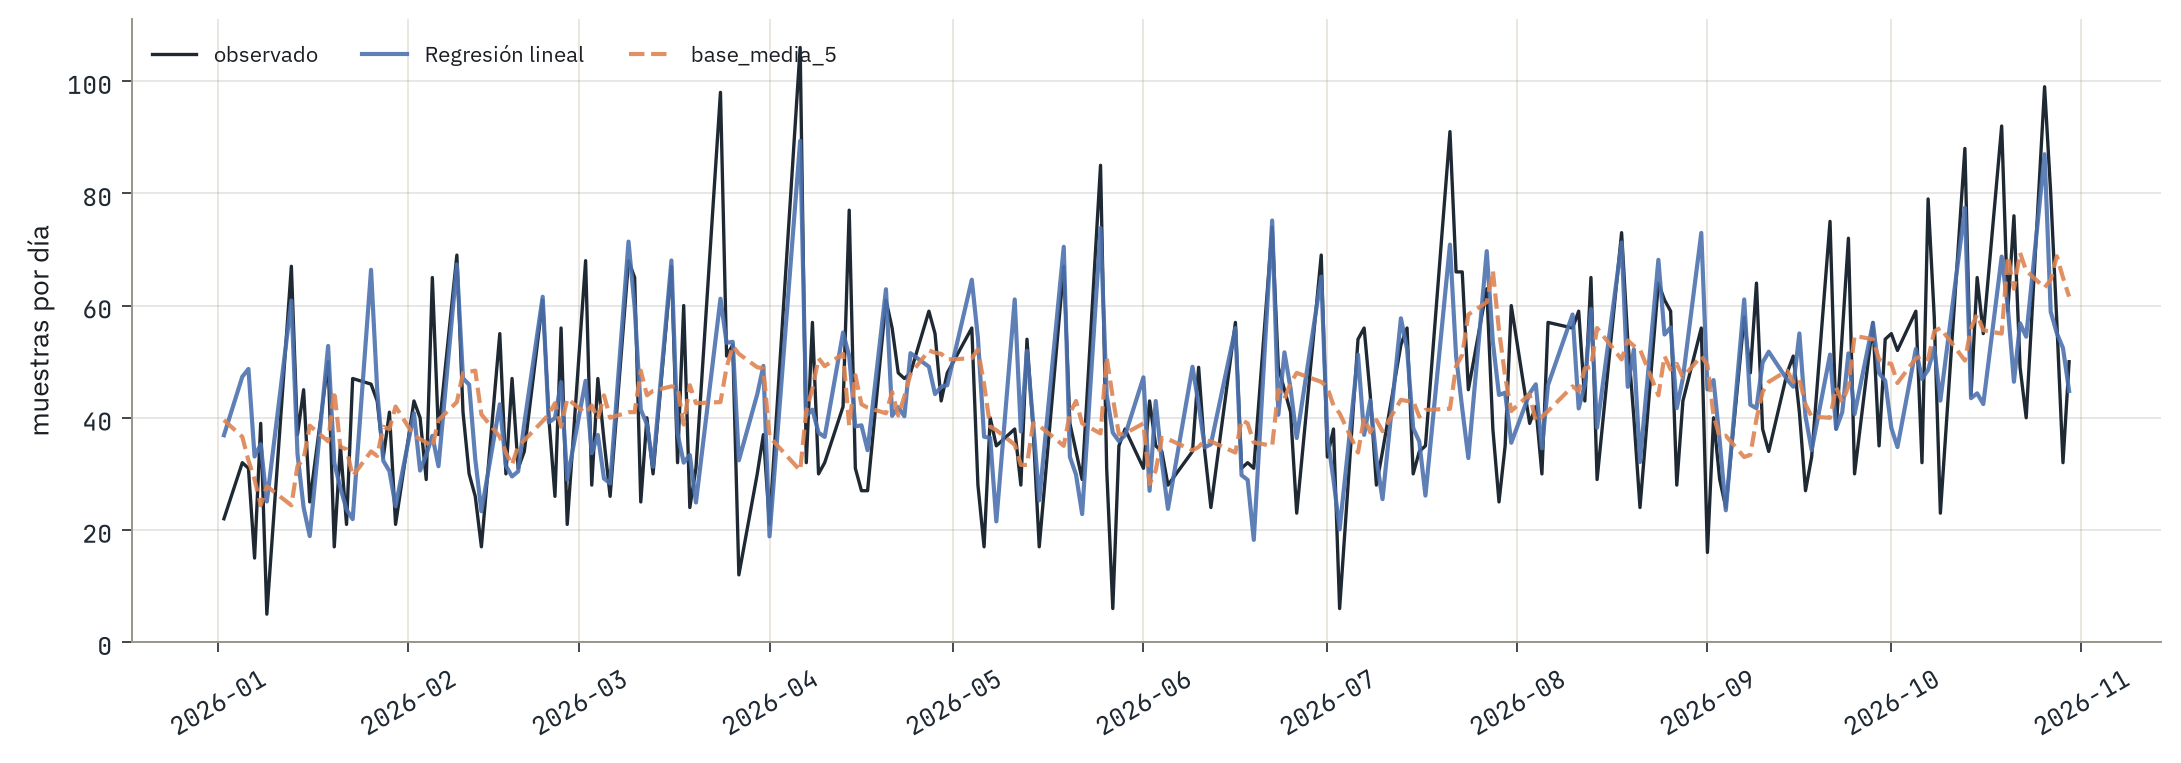
\includegraphics[width=0.85\textwidth]{07_serie_prueba.png}
\caption{Serie de prueba: observado (negro), regresión lineal congelada (azul)
y media de los cinco días anteriores (naranja). Conviene mirar los primeros
días de enero, donde el modelo sobreestima la carga, y los picos aislados, que
ningún predictor anticipa.}
\label{fig:final-serie}
\end{figure}

El error no es uniforme en el tiempo (Figura~\ref{fig:final-serie}): en los
\FinDiasFinDeAnio{} días hábiles de la ventana de fin de año, el residuo medio
es de \FinResiduoFinDeAnio{} muestras (el modelo predice de más), frente a
\FinResiduoResto{} en el resto, lo que indica que el calendario del modelo no
captura bien el arranque lento de enero. En términos operativos, el
\FinDiasFueraPct{}\,\% de los días queda fuera de la tolerancia práctica,
frente al \FinDiasFueraReferenciaPct{}\,\% de la referencia.

\subsection{Clasificación}

La regresión logística calibrada mantuvo su capacidad de ordenar, con un
ROC-AUC de \FinAUCPrueba{} (IC 95\,\% de \FinAUCPruebaInf{} a
\FinAUCPruebaSup{}) frente a \ClfAUCValidacion{} en validación, y su
calibración, con una probabilidad media de \FinProbMediaPrueba{} frente a una
tasa real de \FinPrevalenciaPrueba{} y un Brier de \FinBrierPrueba{}
(Tabla~\ref{tab:final-clf}). Con el umbral congelado ($t=\FinUmbral$) la
precisión casi no cambió (\FinPrecisionPrueba{}, de \FinPrecisionPruebaInf{}
a \FinPrecisionPruebaSup{}), pero el recall bajó de \ClfRecallUmbral{} a
\FinRecallPrueba{} (de \FinRecallPruebaInf{} a \FinRecallPruebaSup{}), con
$\text{TP}=\FinTP$, $\text{FP}=\FinFP$, $\text{FN}=\FinFN$ y
$\text{TN}=\FinTN$ en las \FinMuestrasPrueba{} muestras con resultado.

\begin{table}[!htbp]
\centering
\small
\tablagen{final_clasificacion_validacion}
\caption{Clasificación: validación frente a prueba con el umbral congelado,
con intervalo bootstrap de 95\,\% en prueba.}
\label{tab:final-clf}
\end{table}

Las alertas bajaron a \FinAlertasSemana{} por semana en las
\FinSemanasPrueba{} semanas de prueba (frente a \ClfAlertasSemana{} en
validación), en parte porque llegan menos muestras por día. El costo fue de
\FinCostoPrueba{} (\FinCostoPorMuestraPrueba{} por muestra), frente a
\FinCostoNoAlertar{} de no alertar y \FinCostoAlertarTodo{} de alertar todo,
un ahorro del \FinAhorroPct{}\,\% frente a la mejor política sin modelo, algo
menor que el \ClfAhorroPct{}\,\% de validación.

\paragraph{Umbral retrospectivo (no se usa).} Mirando la prueba, el umbral de
menor costo habría sido \FinUmbralRetro{}, con un costo de \FinCostoRetro{}
frente a \FinCostoPrueba{} del umbral congelado. Se reporta solo para medir
cuánto se pierde por decidir sin ver la prueba, una diferencia pequeña, y
\textbf{no se adopta}, porque elegirlo con la prueba invalidaría la
evaluación.

\subsection{Probabilidad de falso positivo}

En prueba, los \FinReensayados{} positivos reensayados dieron un
\FinReensayoConformeObservadoPct{}\,\% de reensayos conformes (Wilson de
\FinReensayoConformeObservadoInfPct{}\,\% a
\FinReensayoConformeObservadoSupPct{}\,\%), y la capa bayesiana, con la
sensibilidad y la especificidad del desarrollo, anticipaba un
\FinReensayoConformeEsperadoPct{}\,\%, dentro de ese intervalo. El VPP$(x)$
medio de los positivos de prueba es de \FinVPPxMedio{}, es decir, uno de cada
\FinUnoDeCadaFalso{} positivos sería falso. La regla de reensayo se sostiene: bajo el borde, el \FinReglaTasaBajoPct{}\,\% de
los reensayos fue conforme (Wilson de \FinReglaTasaBajoInfPct{}\,\% a
\FinReglaTasaBajoSupPct{}\,\%, con \FinReglaBajoBorde{} de los
\FinReglaReensayosConRecuento{} reensayos con recuento), frente al
\FinReglaTasaAltoPct{}\,\% sobre él, y el grupo concentró el
\FinReglaCapturaPct{}\,\% de los reensayos conformes.

Por ensayo, \FinEnsayosPocosPositivos{}
ensayos tienen menos de \FinMinimoPositivos{} positivos en prueba
(\textit{Salmonella} y esterilidad), así que sus fracciones observadas son
poco precisas y no se interpretan. En la auditoría con la verdad de la
simulación, la fracción de positivos de prueba realmente contaminados es de
\FinAudVPPReal{}, cercana al VPP$(x)$ medio, y el Brier del VPP$(x)$
(\FinAudBrierVPPx{}) vuelve a ser menor que el del VPP por ensayo
(\FinAudBrierVPPEnsayo{}).

\subsection{Resumen}

La Tabla~\ref{tab:final-resumen} reúne las cifras principales. Ninguna se
degradó de forma que invalide el modelo correspondiente, y entre las métricas de desempeño
la que más empeoró es el recall de la clasificación, que conviene vigilar con los datos reales. El
agrupamiento no tiene evaluación en prueba, porque es descriptivo
(\FinAgrK{} perfiles de muestra con silueta \FinAgrSilueta{} y
\FinAgrSegmentos{} segmentos de clientes).

\begin{table}[!htbp]
\centering
\small
\tablagen{final_resumen}
\caption{Resumen final: validación (o desarrollo, en Bayes) frente a prueba.}
\label{tab:final-resumen}
\end{table}

% =====================================================================
% datos_reales.tex
% Responsabilidad única: contar qué encontramos al pasar a la exportación
% real del laboratorio (solo fechas de desarrollo): lotes de Poisson,
% muestras como Poisson compuesta, tamaño de lote por tipo, segmentos,
% riesgo al ingreso y distancia con la simulación.
% Cifras: macros Real*; tablas tabla_real_*; figuras 08_*.
% Si la exportación no estaba al construir, las macros Real* no existen y
% la sección se reduce a una nota.
% =====================================================================
\section{Datos reales: Lotes de Poisson}
\label{sec:datos-reales}

\ifdefined\RealMuestras
Al final del semestre Daniel Arias Mutis, que trabaja en el laboratorio,
consiguió la exportación real con los clientes anonimizados. Nos propuso
clasificar a los clientes por su volumen y a los lotes por su tamaño y nos
dijo que las llegadas le sonaban a un proceso de Poisson. Solo usamos las
fechas de desarrollo (del \RealDesde{} al \RealHasta{}) y dejamos por fuera
todo lo de 2026, que además es donde la base empieza a cambiar. Las
\RealFilas{} filas de la exportación (una por muestra, especificación y
lectura) se vuelven \RealMuestras{} muestras de \RealClientes{} clientes y
\RealLotes{} lotes, donde un lote son las muestras que un cliente ingresa el
mismo día y del mismo tipo (producto o muestreo en planta). El
\RealPlantaPct{}\,\% de las muestras viene de planta y la no conformidad es
de \RealNoConformePct{}\,\%.

\paragraph{Muestras y lotes.} En una Poisson la varianza es igual a la media
así que medimos el índice de dispersión $I = s^2/\bar x$ de los conteos
semanales de cada cliente. Esperábamos que las muestras por semana dieran
cerca de 1 y no fue así: Con los \RealClientesDispersion{} clientes que
tienen al menos \RealMinimoLotes{} lotes la mediana del índice es de
\RealDispMuestrasTodos{} y llega hasta \RealDispMuestrasMax{}. Al contar
lotes en vez de muestras la mediana baja a \RealDispLotesTodos{}
(Figura~\ref{fig:real-dispersion}). Por tipo el índice de los lotes es de
\RealDispLotesProducto{} en producto y \RealDispLotesPlanta{} en planta,
frente a \RealDispMuestrasProducto{} y \RealDispMuestrasPlanta{} en las
muestras (Tabla~\ref{tab:real-dispersion}).

\begin{figure}[!htbp]
\centering
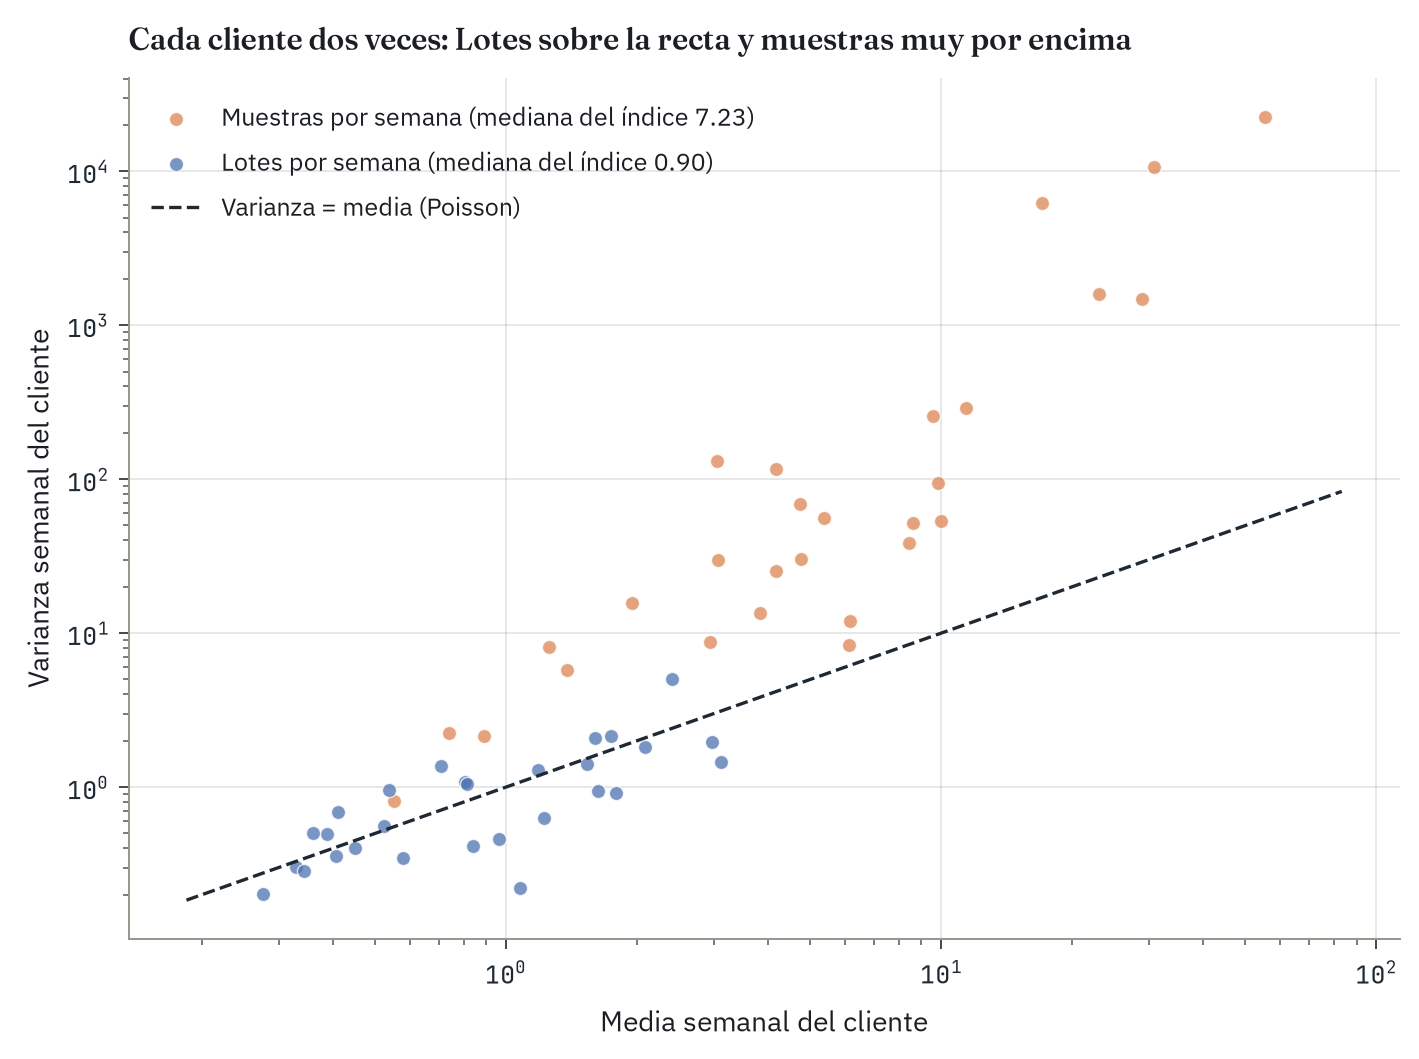
\includegraphics[width=0.7\textwidth]{08_dispersion_clientes.png}
\caption{Media frente a varianza semanal de cada cliente, una vez con sus
muestras y otra con sus lotes, en ejes logarítmicos: Los lotes caen sobre la
recta de Poisson y las muestras quedan muy por encima.}
\label{fig:real-dispersion}
\end{figure}

\begin{table}[!htbp]
\centering
\tablaancha{real_dispersion}
\caption{Índice de dispersión semanal por cliente y tipo de lote, con la
proporción de clientes en que la prueba de dispersión da un valor p menor
que \RealNivel{}: La sobredispersión está en las muestras y no en los lotes.}
\label{tab:real-dispersion}
\end{table}

La explicación es que las muestras son una Poisson compuesta: Si llegan
$N \sim \mathrm{Poisson}(\lambda)$ lotes y el lote $i$ trae $X_i$ muestras,
el total $S = \sum_{i=1}^{N} X_i$ tiene $E[S] = \lambda E[X]$ y
$\mathrm{Var}[S] = \lambda E[X^2]$, de modo que su índice es
$E[X^2]/E[X]$ y crece con la variación del tamaño de lote. Con los lotes de
cada cliente esa cuenta da medianas de \RealCompuestoProducto{} en producto y
\RealCompuestoPlanta{} en planta, del mismo orden que lo observado.

\paragraph{Tamaño de lote.} Modelamos el tamaño como uno más un conteo y
comparamos con el AIC tres opciones (Tabla~\ref{tab:real-tamano} y
Figura~\ref{fig:real-tamano}). En producto los lotes son pequeños (media
\RealLoteMediaProducto{}, mediana \RealLoteMedianaProducto{}) y gana la
\RealLoteMejorProducto{} con $r = \RealLoteRProducto$, aunque la geométrica
queda a solo \RealLoteDeltaGeoProducto{} de AIC. En planta la media es
\RealLoteMediaPlanta{}, la mediana \RealLoteMedianaPlanta{} y el máximo
\RealLoteMaxPlanta{} muestras en un día así que la cola larga de la
\RealLoteMejorPlanta{} ($r = \RealLoteRPlanta$) le saca
\RealLoteDeltaGeoPlanta{} de AIC a la geométrica. Las \RealCampanas{}
campañas de muestreo en planta duran casi siempre un solo día
(\RealCampanaUnDiaPct{}\,\%).

\begin{figure}[!htbp]
\centering
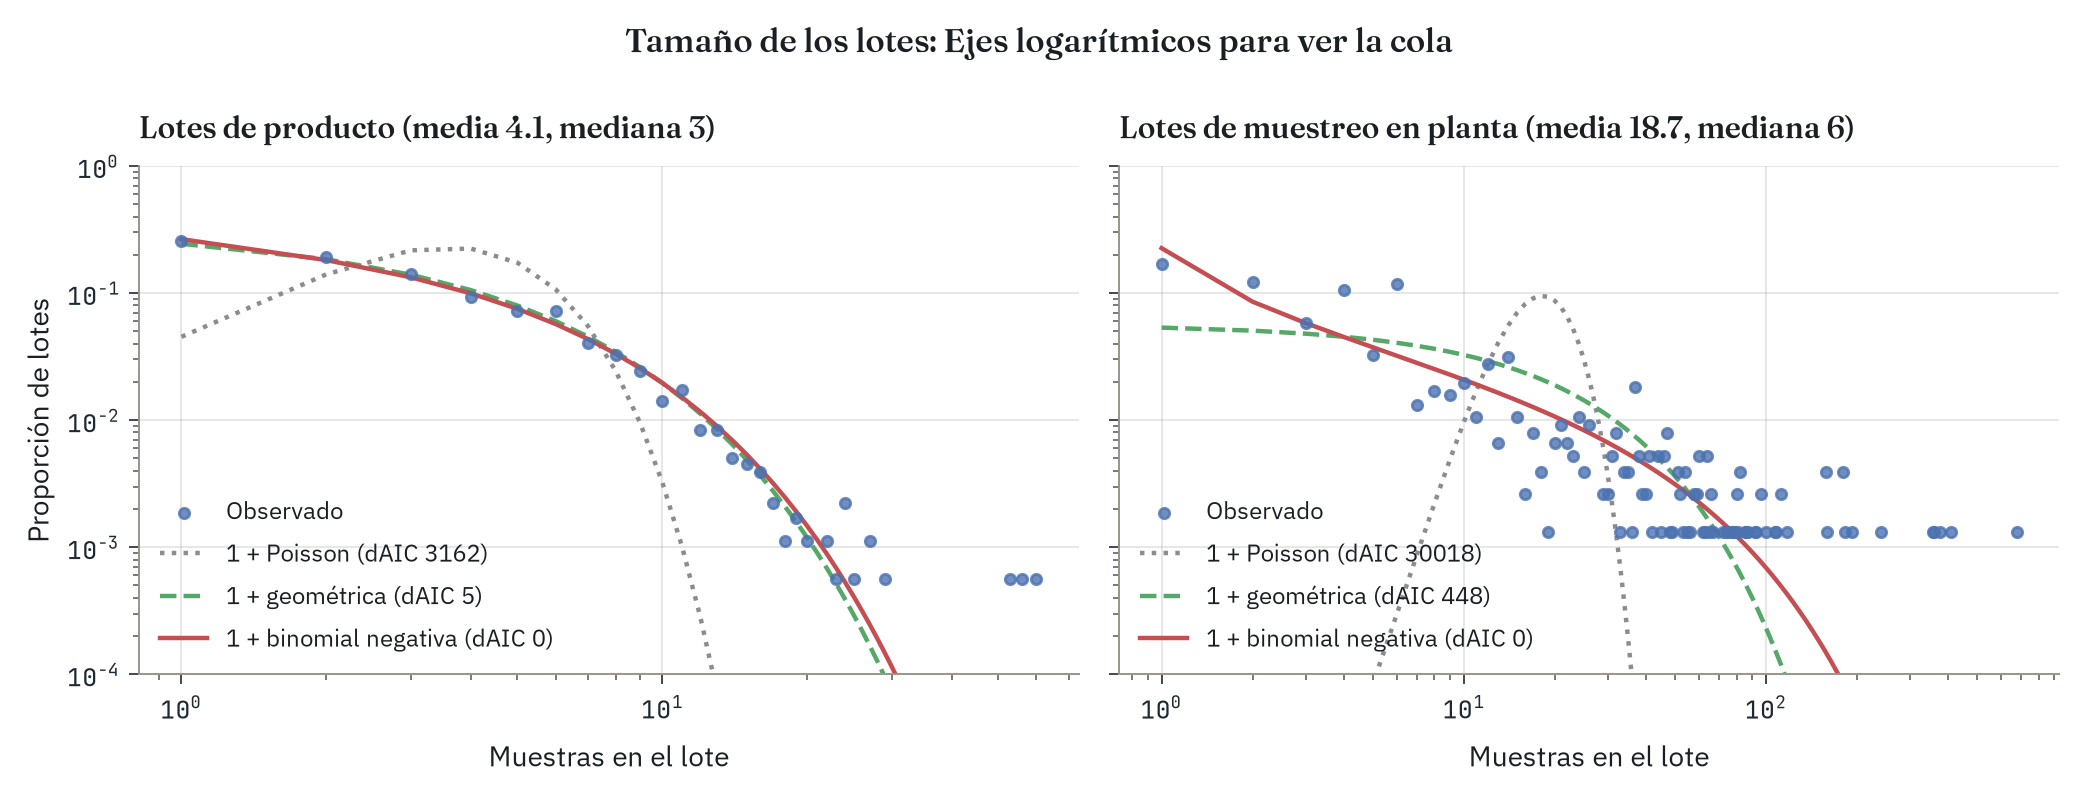
\includegraphics[width=\textwidth]{08_tamano_lote.png}
\caption{Proporción de lotes de cada tamaño con los tres modelos ajustados,
en ejes logarítmicos: Uno más una Poisson no alcanza la cola en ningún tipo y
la binomial negativa sigue los datos.}
\label{fig:real-tamano}
\end{figure}

\begin{table}[!htbp]
\centering
\tablaancha{real_tamano_lote}
\caption{Modelos del tamaño de lote por tipo: La binomial negativa tiene el
menor AIC en los dos.}
\label{tab:real-tamano}
\end{table}

\paragraph{Segmentos y riesgo.} Con el procedimiento de la
Sección~\ref{sec:agrupamiento} sobre \RealSegClientes{} clientes (al menos
\RealSegMinimoMuestras{} muestras) la silueta eligió \RealSegK{} segmentos
(silueta \RealSegSilueta{}). El que más pesa es ``\RealSegMayor'', que trae
el \RealSegMayorMuestrasPct{}\,\% de las muestras. Para el riesgo de no
conformidad al ingreso ajustamos en entrenamiento y medimos en validación
(prevalencia de \RealRiesgoPrevalenciaPct{}\,\%): La regresión logística da
un ROC-AUC de \RealRiesgoAUCLogistica{} (precisión media
\RealRiesgoAPLogistica{}) y el árbol \RealRiesgoAUCArbol{}
(\RealRiesgoAPArbol{}), frente a \RealRiesgoAPBase{} de precisión media de la
línea base. La tasa histórica del cliente sola ya logra
\RealRiesgoAUCHistoria{} así que la señal es real pero modesta.

\paragraph{La simulación.} Nuestra simulación ya generaba lotes de Poisson
con varias muestras cada uno así que la estructura era la correcta. Lo que no
reproduce es el tamaño: Con uno más una Poisson el índice de las muestras
queda entre \RealSimIndiceBajo{} y \RealSimIndiceAlto{}, lejos de la cola de
planta. Separar producto y planta y sacar el tamaño de una binomial negativa
la acercaría. Lo dejamos propuesto porque las secciones anteriores están
cerradas sobre la simulación actual.
\else
Esta versión del informe se construyó sin la exportación real del
laboratorio (el archivo es confidencial y no viaja con el proyecto) así que
la sección no tiene cifras.
\fi

% =====================================================================
% conclusiones.tex
% Responsabilidad única: responder las preguntas del laboratorio con las
% cifras de prueba, proponer acciones modestas, declarar limitaciones y
% trazar el trabajo futuro con la exportación real. Cifras: macros Fin*.
% =====================================================================
\section{Conclusiones, limitaciones y trabajo futuro}
\label{sec:conclusiones}

\subsection{Respuestas a las preguntas del laboratorio}

\begin{itemize}
    \item \textbf{Carga diaria:} una regresión lineal con calendario, puntos de
          muestreo programados y medias móviles predice la carga del día con
          un error absoluto medio de \FinMAEPrueba{} muestras sobre una media
          de \FinMediaPrueba{}, y una habilidad de \FinHabilidadPrueba{} frente
          a la media de los cinco días anteriores; aun así, el
          \FinDiasFueraPct{}\,\% de los días queda fuera de la tolerancia
          práctica.
    \item \textbf{Riesgo de no conformidad:} una regresión logística calibrada,
          con el umbral \FinUmbral{} que dicta la razón de costos, ordena las
          muestras con un ROC-AUC de \FinAUCPrueba{} y emite unas
          \FinAlertasSemana{} alertas por semana, de las cuales acierta una
          fracción de \FinPrecisionPrueba{} y que detectan una fracción de
          \FinRecallPrueba{} de las no conformes, con un ahorro del
          \FinAhorroPct{}\,\% frente a no alertar.
    \item \textbf{Falso positivo:} según los controles y el clasificador, uno de
          cada \FinUnoDeCadaFalso{} positivos sería falso, cifra que la
          fracción de reensayos conformes de prueba confirma
          (\FinReensayoConformeObservadoPct{}\,\% observada frente a
          \FinReensayoConformeEsperadoPct{}\,\% esperada), y los reensayos
          conformes se concentran en los recuentos que superan el límite en
          menos de \ClfReglaVecesLimite{} veces.
    \item \textbf{Grupos:} existen \FinAgrK{} perfiles de muestra y
          \FinAgrSegmentos{} segmentos de clientes, estables entre semillas
          pero con fronteras difusas (silueta de \FinAgrSilueta{}), útiles
          para describir, no para decidir de forma automática.
\end{itemize}

\subsection{Recomendaciones}

Las recomendaciones son deliberadamente modestas, porque las cifras vienen de
datos simulados y lo primero es comprobarlas con los reales:

\begin{itemize}
    \item \textbf{Planeación de turnos:} usar la predicción diaria como apoyo
          para asignar personal de recepción y siembra, con una revisión manual
          en las primeras semanas del año, donde el modelo sobreestima.
    \item \textbf{Piloto de alertas en recepción:} marcar las muestras que
          superan el umbral durante algunas semanas, sin cambiar el flujo,
          y medir con los datos reales la precisión, el recall y la carga de
          alertas por semana antes de adoptarlas.
    \item \textbf{Regla de reensayo:} priorizar el reensayo de los no conformes
          cuyo recuento quede por debajo de \ClfReglaVecesLimite{} veces el
          límite, que es donde se concentran los reensayos conformes.
    \item \textbf{Seguimiento de clientes:} revisar con el área comercial y de
          calidad el segmento con más no conformidad y más entregas tardías.
\end{itemize}

\subsection{Limitaciones}

\begin{itemize}
    \item \textbf{Datos simulados:} las métricas muestran que el procedimiento
          funciona de punta a punta y que no hay fugas, pero no miden la
          operación real; el generador fija relaciones que los modelos luego
          encuentran, así que con datos reales las habilidades pueden ser más
          modestas, y las razones de odds o los perfiles no deben leerse como
          hallazgos sobre el laboratorio.
    \item \textbf{Pocos casos en algunos ensayos:} \textit{Salmonella} y
          esterilidad tienen pocos positivos, de forma que su VPP y su
          fracción de reensayos conformes tienen intervalos anchos y, en
          prueba, no se interpretan.
    \item \textbf{Reensayo como referencia:} un reensayo conforme no equivale a
          un falso positivo, porque el reensayo también falla; con datos
          reales no existe otra verdad contra la cual comparar.
    \item \textbf{Siluetas bajas:} los grupos tienen fronteras difusas y la
          silueta del cribado no era comparable con la del estudio a fondo,
          por un cambio de preprocesamiento que el cribado debió compartir.
    \item \textbf{Intervalos bootstrap:} remuestrean filas como si fueran
          independientes, lo que en la serie diaria ignora la autocorrelación
          y hace que los intervalos de la regresión sean probablemente
          demasiado estrechos.
    \item \textbf{Un solo corte de prueba:} la prueba cubre un único periodo
          (\FinPruebaDesde{} a \FinPruebaHasta{}), así que las diferencias
          entre validación y prueba mezclan el desempeño del modelo con los
          cambios de nivel de la serie.
\end{itemize}

\subsection{Trabajo futuro con la exportación real}

El siguiente paso es conectar la exportación real, que solo requiere copiar
los archivos, completar el mapeo de columnas y reconstruir los notebooks,
revisar primero la tabla de cobertura y la auditoría de limpieza, y ajustar
las fechas de corte para que caigan dentro del periodo exportado. Después,
conviene repetir el cribado con el mismo preprocesamiento del estudio a
fondo, usar intervalos por bloques (bootstrap de bloques móviles) en la serie
diaria y, si el piloto de alertas confirma su utilidad, recalibrar el modelo
periódicamente, ya que la tasa de no conformidad cambia con la mezcla de
clientes.


\bibliographystyle{plain}
{\small\bibliography{referencias}}

% El apéndice sigue a las referencias en la misma página (ahorra una hoja casi vacía).
\appendix
% =====================================================================
% apendice.tex
% Responsabilidad única: documentar la reproducibilidad (entorno, semilla,
% comandos y comprobaciones automáticas) y la arquitectura por capas del
% paquete. Sin resultados.
% =====================================================================
\section{Reproducibilidad y arquitectura}
\label{sec:apendice}

\subsection{Reproducibilidad}

Todo el proyecto se reconstruye desde la carpeta raíz con \codigo{uv} y
Python 3.12. Cada paso aleatorio parte de la semilla \DatSemilla{} así que
dos ejecuciones dan las mismas cifras. Con \codigo{make notebooks} se ejecutan las siete
etapas en orden y se regenera \codigo{informe/generado/} (las macros, el
índice y las tablas), con \codigo{make colab} los notebooks se copian a una
carpeta vacía y se ejecutan allí sin el paquete para probar que se valen por
sí solos y con \codigo{make pdf} (en \codigo{informe/}) se compila este
documento. Por último \codigo{make verificar} corre el guion
\codigo{verificar.py} de la carpeta \codigo{verificacion/}. Ese guion revisa
la regla de capas, que el generador sea determinista, la ortogonalidad del
L16, las fórmulas de Bayes contra un cálculo a mano, que no haya fugas por
momento, que solo la etapa~07 lea la prueba, que las etapas no tengan cifras
escritas a mano y que no falten macros en el informe.

En Google Colab basta con subir \codigo{notebooks/Proyecto\_Final.ipynb} y
ejecutarlo todo porque su primera sección recrea el paquete. Lo probamos con
una pila parecida a la de Colab (pandas 2.2 y scikit-learn 1.6) y con la local
(pandas 3 y scikit-learn 1.9).

\subsection{Arquitectura por capas}

Cada subcarpeta de \codigo{proyecto/} es una capa y un módulo solo importa de
su capa o de una menor (Tabla~\ref{tab:capas}). Las etapas se comunican solo
por archivos.

\begin{table}[!htbp]
\centering
\small
\begin{tabular}{clp{10.4cm}}
\toprule
Capa & Carpeta & Responsabilidad \\
\midrule
0 & \codigo{base} & Configuración, rutas, artefactos entre etapas y custodia de la prueba \\
1 & \codigo{datos} & Contrato de columnas, festivos, carga, mapeo de la exportación y simulación \\
2 & \codigo{preparacion} & Limpieza determinista, integración de tablas y partición temporal \\
3 & \codigo{variables} & Tablas de modelado con el momento de cada variable (sin fugas) \\
4 & \codigo{modelos} & Tuberías de scikit-learn, modelos, rejillas y agrupamiento \\
5 & \codigo{evaluacion} & Validación por bloques, métricas, umbral por costo, bootstrap y Bayes \\
6 & \codigo{cribado} & Catálogo de análisis, cribado rápido, arreglo L16 y corridas de Taguchi \\
7 & \codigo{reporte} & Figuras, componentes HTML y exportación de cifras y tablas a \LaTeX{} \\
8 & \codigo{etapas} & Una función por sección de notebook: Calcula, guarda y registra cifras \\
\bottomrule
\end{tabular}
\caption{Capas del paquete \codigo{proyecto/}: Los guiones de los notebooks
solo narran y llaman funciones de la capa~8.}
\label{tab:capas}
\end{table}


\end{document}
